\documentclass[12pt]{article}
\usepackage[margin = 1.5in]{geometry}
\setlength{\parindent}{0in}
\usepackage{amsfonts, amssymb, amsthm, mathtools, tikz, qtree, float}
\usepackage[lined]{algorithm2e}
\usepackage[T1]{fontenc}
\usepackage{ae, aecompl, color}
\usepackage[pdftex, pdfauthor={Charles Shen}, pdftitle={CS 251: Computer Organization and Design}, pdfsubject={Lecture notes from CS 251: Computer Organization and Design at the University of Waterloo}, pdfkeywords={CS 251, course notes, notes, Waterloo, University of Waterloo}, pdfproducer={LaTeX}, pdfcreator={pdflatex}]{hyperref}
\usepackage{cleveref}
\usepackage{wrapfig}
\usepackage{multicol, multirow, array}

\DeclarePairedDelimiter{\set}{\lbrace}{\rbrace}

\definecolor{darkish-blue}{RGB}{25,103,185}

\hypersetup{
  colorlinks,
  citecolor=darkish-blue,
  filecolor=darkish-blue,
  linkcolor=darkish-blue,
  urlcolor=darkish-blue
}

\theoremstyle{definition}
\newtheorem*{defn}{Definition}
\newtheorem*{theorem}{Theorem}
\newtheorem*{corollary}{Corollary}
\newtheorem{ex}{Example}[section]

\crefname{ex}{Example}{Example}

\setlength{\marginparwidth}{1.5in}
\newcommand{\lecture}[1]{
  \marginpar{{
    \footnotesize $\leftarrow$ \underline{#1}}
  }
}

\newcommand{\includePicture}[3]{
  \begin{figure}[!ht]
  \centering
  \scalebox{#1}{\includegraphics{#2}}
  \caption{#3}
  \end{figure}
}

\newcolumntype{L}[1]{>{\raggedright\let\newline\\\arraybackslash\hspace{0pt}}m{#1}}
\newcolumntype{C}[1]{>{\centering\let\newline\\\arraybackslash\hspace{0pt}}m{#1}}
\newcolumntype{R}[1]{>{\raggedleft\let\newline\\\arraybackslash\hspace{0pt}}m{#1}}

\allowdisplaybreaks

\makeatletter
\def\blfootnote{\gdef\@thefnmark{}\@footnotetext}
\makeatother

%%%%%%%%%%%%%%%%%%%%%
%% D O C U M E N T %%
%%%%%%%%%%%%%%%%%%%%%

\begin{document}
  \let\ref\Cref

  \title{\bf{CS 251: Computer Organization and Design}}
  \date{Spring 2016, University of Waterloo \\ \center Notes written from Safaa Bedawi's lectures.}
  \author{Charles Shen}

  \blfootnote{Feel free to email feedback to me at
  \href{mailto:echen902@gmail.com}{echen902@gmail.com}.}

  \maketitle
  \newpage
  \tableofcontents
  \newpage

  \section{Performance}
  \subsection{Defining Performance}
  Performance can be defined in terms of more than just speed.
  Different performance metrics are required for different scenarios.
  To an individual, the performance in interest is \emph{response time}---the time between the start and completion of a task---also referred to as \emph{execution time}. \\
  To a data-center manager, the interest is in \emph{throughput} or \emph{bandwidth}---the total amount of work done in a given time.

  \subsection{Measuring Performance}
  Time is the measure of computer performance; the computer that performs the same amount of work in the least time is the fastest. \\
  Program execution time is measured in seconds per program, this is usually known as \emph{elapsed time, wall clock time, \emph{or} response time}. \\

  Computers are often shared, so a processor may work on several programs simultaneously.
  In which, the system attempts to optimize throughput rather than attempting to minimize the elapsed time for a program. \\

  The \emph{CPU execution time}, also knowns as \emph{CPU time}, makes the distinction between the elapsed time and the actual time the CPU spends computing for a specific task. \\
  Further distinction can be made, \emph{user CPU time}, the CPU time spent in the program, and \emph{system CPU time}, the CPU time spent in the operating system performing tasks on behalf of the program. \\

  Another measure of performance is using a measure that relates to how fast the hardware can perform basic functions. \\
  Almost all computers are constructed using a clock that determines when events take place in the hardware.
  These discrete time intervals are called \emph{clock cycles} (or ticks, clock ticks, clock periods, clocks, cycles). \\
  The length of a clock period can be either the time for a complete clock cycle (e.g. 250 picoseconds, or 250 ps) or the clock rate (e.g. 4 gigahertz, or 4GHz), which is the inverse of the clock period.
  $$1ps = 1 \times 10^{-12} = \frac{1}{1,000,000,000,000}$$

  \subsection{CPU Performance and Its Factors}
  \begin{align*}
  \parbox{4cm}{CPU execution time\\for a program}
  &= ~\parbox{3.5cm}{CPU clock cycles\\for a program} \times \text{ Clock cycle time} \\
  &= \frac{\text{CPU clock cycles for a program}}{\text{Clock rate}}
  \end{align*}

  \subsection{Instruction Performance}
  $$\text{CPU clock cycles} = ~\parbox{3cm}{Instructions for\\a program} \times ~\parbox{4cm}{Average clock cycles\\per instruction}$$
  \emph{Clock cycles per instruction}, which is the average number of clock cycles each instruction takes to execute, is often abbreviated as \emph{CPI}. \\
  CPI is an average of all the instructions executed in the program because different instructions may take different amounts of time depending on what they do.

  \subsection{The Classic CPU Performance Equation}
  $$\text{CPU time} = \text{Instruction count} \times \text{CPI} \times \text{Clock cycles time}$$
  Note that CPU varies by \emph{instruction mix}, which is a measure of the dynamic frequency of instructions across one or many programs.

  \newpage

  \section{From Zero To One, Abstractions}
  \includePicture{0.6}{pictures/abstractionLevel.png}{Levels of abstraction for electronic computing system}

  \subsection{The Three -Y's}
  \begin{itemize}
    \item [\textbf{Hierarchy}] involves dividing a system into modules, then further subdividing each of these modules until the pieces are easy to understand
    \item [\textbf{Modularity}] states that the modules have well-defined functions and interfaces, so that they connect together easily without unanticipated side effects
    \item [\textbf{Regularity}] seeks uniformity among the modules. Common modules are reused many times, reducing the number of distinct modules that must be designed
  \end{itemize}

  \subsection{Hexadecimal Number System}
  \begin{tabular} {c | c | c}
  Hexadecimal Digit & Decimal Digit & Binary Equivalent \\ \hline \hline
  0 & 0 & 0000 \\ \hline
  1 & 1 & 0001 \\ \hline
  2 & 2 & 0010 \\ \hline
  3 & 3 & 0011 \\ \hline
  4 & 4 & 0100 \\ \hline
  5 & 5 & 0101 \\ \hline
  6 & 6 & 0110 \\ \hline
  7 & 7 & 0111 \\ \hline
  8 & 8 & 1000 \\ \hline
  9 & 9 & 1001 \\ \hline
  A & 10 & 1010 \\ \hline
  B & 11 & 1011 \\ \hline
  C & 12 & 1100 \\ \hline
  D & 13 & 1101 \\ \hline
  E & 14 & 1110 \\ \hline
  F & 15 & 1111 \\
  \end{tabular}

  \subsection{Bytes, Nibbles, and All That Jazz}
  A group of eight bits is called a \emph{byte}. Represents $256 = 2^{8}$ possibilities. \\
  A group of four bits is called a \emph{nibble}. Represents $16 = 2^{4}$ possibilities. \\
  A microprocessor is a processor built on a single chip. \\
  Microprocessors handle data in chunks called words. The size of a word depends on the architecture of the microprocessor. \\
  Within a group of bits, the bit in the 1's column is called the least significant bit (lsb), and the bit at the other end is called the most significant bit (msb). \\
  Within a word, the bytes are identified as least significant byte (LSB) through most significant byte (MSB). \\

  \blfootnote{When adding operands with different signs, overflow cannot occur because the sum must be no larger than one of the operands.}
  \newpage
  \subsection{Logic Gates}
  A circuit element that performs a basic logic function \\ \\
  \textbf{Single Input} \\
  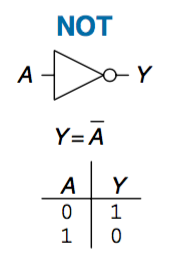
\includegraphics[scale=0.9]{pictures/notGate.png}
  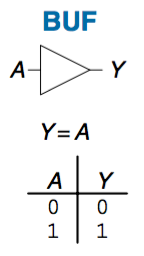
\includegraphics[scale=0.9]{pictures/bufGate.png} \\
  \textbf{Double Output} \\
  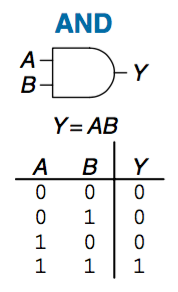
\includegraphics[scale=0.9]{pictures/andGate.png}
  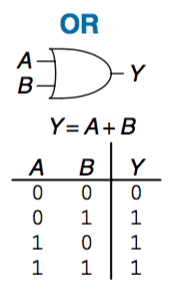
\includegraphics[scale=0.9]{pictures/orGate.png}
  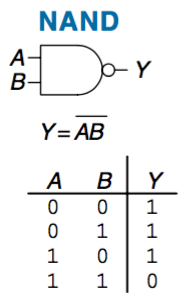
\includegraphics[scale=0.9]{pictures/nandGate.png}
  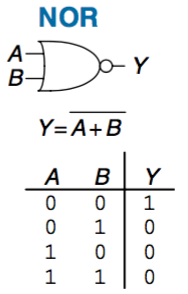
\includegraphics[scale=0.9]{pictures/norGate.png}
  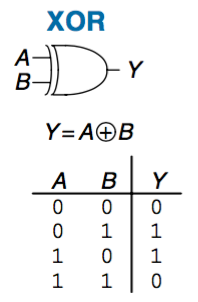
\includegraphics[scale=0.9]{pictures/xorGate.png}

  \subsection{Beneath the Digital Abstraction}
  A digital system uses discrete-valued variables. \\
  Variables are represented by continuous physical quantities such as the voltage on a wire, the position of a gear, or the level of fluid in a cylinder.
  \begin{ex}
    Consider representing a binary signal A with a voltage on a wire. \\
    Let 0 volts (V) indicate A = 0 and 5V indicate A = 1. \\
    Any real system must tolerate some noise, so 4.97V probably ought to be interpreted as A = 1 as well. \\
    But what about 4.3V? Or 2.8V? Or 2.5000000V?
  \end{ex}
  \subsubsection{Supply Voltage}
  Suppose the lowest voltage in the system is 0V, also called ground or GND \\
  The highest voltage in the system comes from the power supply and is usually called $V_{DD}$

  \subsubsection{Logic Levels}
  Mapping of a continuous variable onto a discrete binary variable is done by defining logic levels.
  First gate is called the driver and the second gate is called the receiver.
  Output of the driver is connected to the input of the receiver. \\
  The driver produces a LOW (0) output in the range of 0 to $V_{OL}$ or a HIGH (1) output in the range of $V_{OH}$ to $V_{DD}$

  \subsubsection{Noise Margins}
  If the output of the driver is to be correctly interpreted at the input of the receiver, we must choose $V_{OL} < V_{IL}$ and $V_{OH} > V_{IH}$ \\
  Even if the output of the driver is contaminated by some noise, the input of the receiver will still detect the correct logic level.
  Noise margin is the amount of noise that could be added to a worst-case output such that the signal can still be interpreted as a valid input

  \blfootnote{Note: power flows from drain to source.}

  \subsubsection{DC Transfer Characteristics}
  The DC transfer characteristics of a gate describe the output voltage as a function of the input voltage when the input is changed slowly enough that the output can keep up. \\
  Called transfer characteristics because they describe the relationship between input and output voltages.

  \newpage

  \section{CMOS Transistors}
  Transistors are electrically controlled switches that turn ON or OFF when a voltage or current is applied to a control terminal. \\
  Two main types of transistors are bipolar transistors and metal-oxide-semiconductor field effect transistors (MOSFETs or MOS transistors).

  \subsection{Semiconductors}
  MOS transistors are built from silicon. \\
  Silicon has four electrons in its valence shell and forms bonds with four adjacent atoms, resulting in a crystalline lattice. \\
  By itself, silicon is a poor conductor due to all the electrons are tied up in covalent bonds. \\
  Becomes a better conductor when small amounts of impurities, called dopant atoms, are added. \\
  The conductivity of silicon changes over many orders and of magnitude depending on the concentration of dopants, silicon is called a semiconductor. \\
  \textbf{Add Arsenic} \\
  If arsenic (As), a group V dopant, is added, the dopant atoms have an extra electron that is not involved in the bonds. \\
  Electron can easily move about the lattice, leaving an ionized dopant atom (As+) behind. \\
  Electron carries a negative charge, so arsenic is an n-type dopant. \\
  \textbf{Add Boron} \\
  If boron (B), a group III dopant, is added, the dopant atoms are missing an electron. \\
  The missing electron is called a hole. \\
  An electron from a neighboring silicon atom may move over to fill the missing bond, forming an ionized dopant atom (B-) and leaving a hole at the neighboring silicon atom. \\
  The hole can migrate around the lattice. \\
  Hole is a lack of negative charge, so it acts like a positively charged particle. \\
  So boron is a p-type dopant.

  \subsection{Diodes}
  \begin{wrapfigure}{r}{0.25\textwidth}
    \centering
    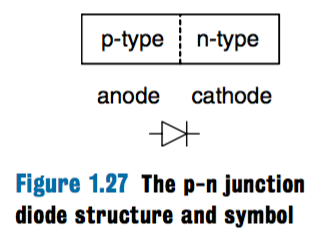
\includegraphics[width=0.25\textwidth]{pictures/diode.png}
  \end{wrapfigure}
  Junction between p-type and n-type silicon is called a diode.
  The p-type region is called the anode and the n-type region is called the cathode. \\
  When the voltage on the anode rises above the voltage on the cathode, the diode is forward biased, and current flows through the diode from the anode to the cathode. \\
  When the anode voltage is lower than the voltage on the cathode, the diode is reverse biased, and no current flows. \\
  The diode symbol intuitively shows that current only flows in one direction.

  \subsection{Capacitors}
  A \emph{capacitor} consists of two conductors separated by an insulator. \\
  When a voltage $V$ is applied to one of the conductors, the conductor accumulates electric \emph{charge} $Q$ and the other conductor accumulates the opposite charge $-Q$. \\
  The \emph{capacitance} C of the capacitor is the ratio of charge to voltage: $C = \frac{Q}{V}$.
  The capacitance is proportional to the size of the conductors and inversely proportional the distance between them. \\
  Capacitance is important because charging or discharging a conductor takes time and energy. More capacitance means that a circuit will be slower and require more energy to operate.

  \subsection{nMOS and pMOS Transistors}
  \begin{center}
    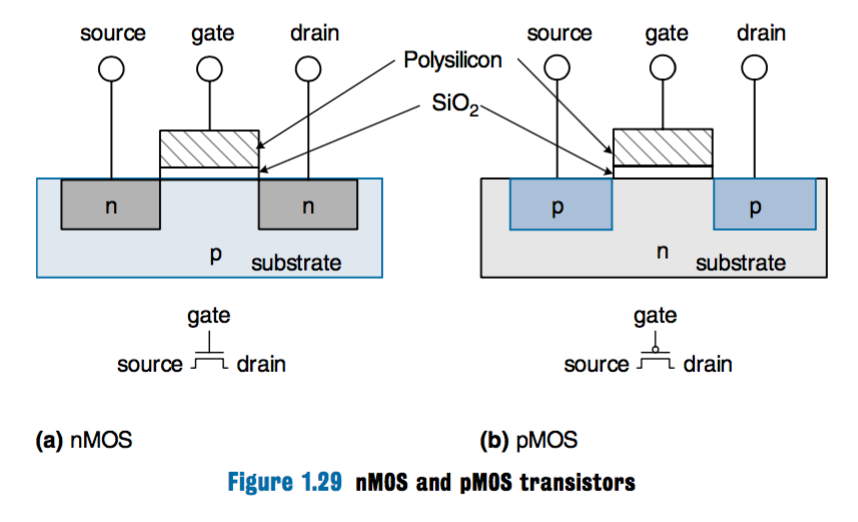
\includegraphics[width=0.8\textwidth]{pictures/nMOSpMOS.png}
  \end{center}
  A MOSFET is a sandwich of several layers of conducting and insulating materials. \\
  There are two flavors of MOSFETs: nMOS and pMOS. \\
  The n-type transistors, called \emph{nMOS}, have regions of n-type dopants adjacent tot he gate called the \emph{source} and the \emph{drain} and are built on a p-type semiconductor substrate. \\
  The \emph{pMOS} transistors are just the opposite, consisting of p-type source and drain regions in an n-type \emph{substrate}. \\
  A MOSFET behaves as a voltage-controlled switch in which the gate voltage creates an electric field that turns ON or OFF a connection between the source and drain. \\
  nMOS transistors pass 0's well but passes 1's poorly.
  Similarly, pMOS transistors pass 1's well but 0's poorly. \\
  nMOS transistors need a p-type substrate, and pMOS transistors need an n-type substrate.
  To build both flavors of transistors on the same chip, manufacturing processes typically start with a p-type wafer, then implant n-type region called wells where the pMOS transistors should go.
  These processes that provide both flavors of transistors are called Complementary MOS or CMOS.
  \begin{wrapfigure}{r}{0.5\textwidth}
    \centering
    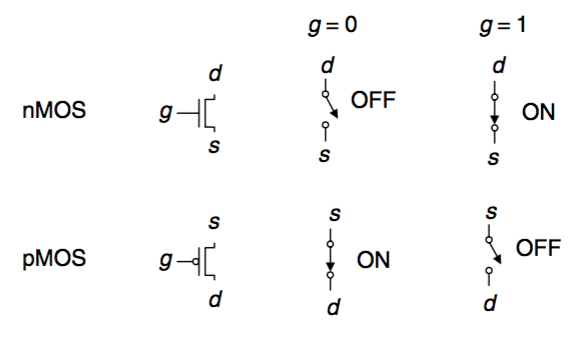
\includegraphics[width=0.5\textwidth]{pictures/nMOSpMOSGate.png}
  \end{wrapfigure}
  CMOS processes are used to build the vast majority of all transistors fabricated today. \\
  CMOS processes provide two types of electrically controlled switches.
  nMOS transistors are OFF when the gate is 0 and ON when the gate is 1.
  pMOS transistors are just the opposite: ON when the gate is 0 and OFF when the gate is 1.

  \subsection{Transmission Gates}
  \begin{wrapfigure}{r}{0.15\textwidth}
    \centering
    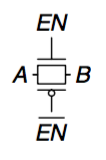
\includegraphics[width=0.15\textwidth]{pictures/transmissionGate.png}
  \end{wrapfigure}
  At times, designers find it convenient to use an ideal switch that can pass both 0 and 1 well. \\
  nMOS transistors are good at passing 0 and pMOS transistors are good at passing 1, so the parallel combination of the two passes both values well. \\
  Image to the right shows such a circuit, called \emph{transmission gate \emph{or} pass gate}. \\
  The two sides of the switch are called \emph{A \emph{and} B} because a switch is bidirectional and has no preferred input or output side.
  The control signals are called \emph{enables}, $EN$ and $\overline{EN}$. \\
  When $EN = 0$ and $\overline{EN} = 1$, both transistors are OFF.
  Hence, the transmission gate is OFF or disabled, so A and B are not connected. \\
  When $EN = 1$ and $\overline{EN} = 0$, the transmission is ON or enabled, and any logic value can flow between A and B.

  \subsection{Pseudo-nMOS Logic}
  An \emph{N}-input CMOS NOR gate uses \emph{N} nMOS transistors in parallel and \emph{N} pMOS transistors in series.
  Transistors in series are slower than transistors in parallel, just as resistors in series have more resistance than resistors in parallel. \\
  Moreover, pMOS transistors are slower than nMOS transistors because holes cannot move around the silicon lattice as fast as electrons.
  Therefore parallel nMOS transistors are fast and the series pMOS transistors are slow, especially when many are in series. \\

  Pseudo-nMOS logic replaces the slow stack of pMOS transistors with a single weak pMOS transistor that is always ON.
  This pMOS transistors is often called a \emph{weak pull-up}.
  The physical dimensions of the pMOS transistor are selected so that the pMOS transistor will pull the output, $Y$, HIGH weakly---that is, only if none of the nMOS transistors are ON.
  But if any nMOS transistor is ON, it overpowers the weak pull-up and pulls Y down close enough to GND to produce a logic 0. \\

  The advantage of pseudo-nMOS logic is that it can be used to build fast NOR gates with many inputs. \\
  The disadvantage is that a short circuit exists between $V_{DD}$ and GND when the output is LOW; the weak pMOS and nMOS transistors are both ON.
  The short circuit draws continuous power, so pseudo-nMOS logic must be used sparingly.

  \newpage
  \section{Summary So Far}
  \emph{There are 10 kinds of people in this world: those who can count in
binary and those who can't.} \\
  The real world is analog, though digital designers discipline themselves to use a discrete subset of possible signals.
  In particular, binary variables have just two states: 0 and 1, also called FALSE and TRUE or LOW and HIGH. \\

  Logic gates compute a binary output from one or more binary inputs.
  Some of the common logic gates are:
  \begin{itemize}
    \item[\textbf{NOT}:] TRUE when all input is FALSE
    \item[\textbf{AND}:] TRUE when all input are TRUE
    \item[\textbf{OR}:]  TRUE when any inputs are TRUE
    \item[\textbf{XOR}:] TRUE when an odd number of inputs are TRUE
  \end{itemize}

  Logic gates are commonly built from CMOS transistors, which behave as electrically controlled switches. \\
  nMOS transistors turn ON when the gate is 1. \\
  pMOS transistors turn ON when the gate is 0.

  \newpage
  \section{Introduction to Combinational Logic Design}
  In digital electronics, a \emph{circuit} is a network that processes discrete-valued variables. \\
  A circuit can be viewed as a black box, with
  \begin{itemize}
    \item one or more discrete-valued \emph{input terminals}
    \item one or more discrete-valued \emph{output terminals}
    \item a \emph{functional specification} describing the relationship between inputs and outputs
    \item a \emph{timing specification} describing the delay between inputs changing and output responding
  \end{itemize}
  Peering inside the black box, circuits are composed of nodes and elements. \\
  An \emph{element} is itself a circuit with inputs, outputs, and a specification. \\
  A \emph{node} is a wire, whose voltage conveys a discrete-valued variable.
  Nodes are classified as \emph{input, output, \emph{or} internal}. \\
  Input receive values from the external world. \\
  Output deliver values to the external world. \\
  Wires that are not inputs or outputs are called internal nodes. \\

  Digital circuits are classified as \emph{combinational \emph{or} sequential}. \\
  A combinational circuit's outputs depend only on the current values of the inputs; in other words, it combines the current input values to compute the output.
  For example, a logic gate is a combinational circuit. \\
  A sequential circuit's outputs depend on both current and previous values of the inputs; in other words, it depends on the input sequence. \\
  A combinational circuit is \emph{memoryless}, but a sequential circuit has \emph{memory}. \\

  The functional specification of a combination circuit expresses the output values in terms of the current input values. \\
  The timing specification of a combinational circuit consists of lower and upper bounds on the delay from input to put. \\

  To simply drawings, a single line with a slash through it and a number next to it is often used to indicate a \emph{bus}, a bundle of of multiple signals. \\

  \begin{wrapfigure}{l}{0.25\textwidth}
    \centering
    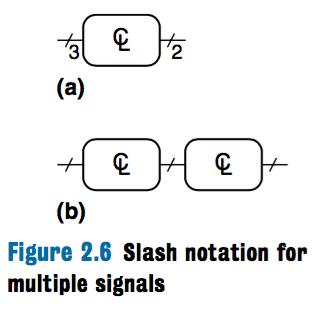
\includegraphics[width=0.25\textwidth]{pictures/busExample.png}
  \end{wrapfigure}
  In Figure 2.6(a), it represents a block of combination logic with three inputs and output outputs. \\
  If the number of bits is unimportant or obvious from the context, the slash may be shown without a number. \\
  Figure 2.6(b) indicates two blocks of combinational logic with an arbitrary number of outputs from one block serving as inputs to the second block. \\

  The rules of \emph{combinational composition} tell us how we can build a large combinational circuit from smaller combinational circuit elements. \\
  A circuit is combinational if it consists of interconnected circuit elements such that:
  \begin{itemize}
    \item Every circuit element is itself combinational
    \item Every node of the circuit is either designated as an input to the circuit or connects to exactly one output terminal of a circuit element
    \item The circuit contains no cyclic paths: every path through the circuit visits each circuit node at most once
  \end{itemize}

  Examples: \\
  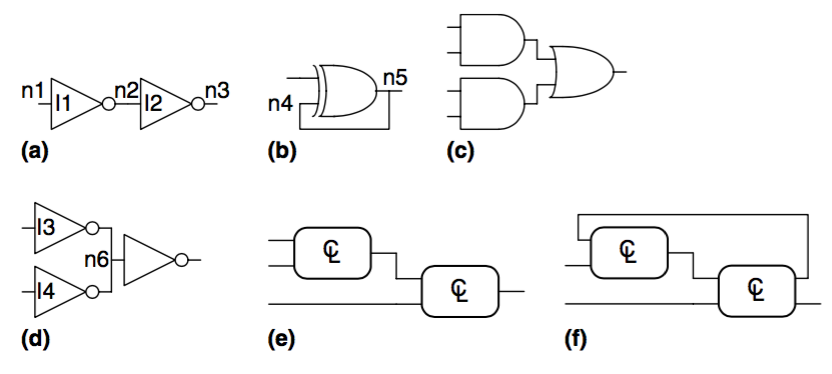
\includegraphics{pictures/combinationalCircuitExample.png}
  (a) is combinational. It is constructed from two combinational circuit elements (inverters $I1$ and $I2$). It has three nodes: $n1$, $n2$, and $n3$. $n1$ is an input to the circuit and to $I1$; $n2$ is an internal node, which is the output of $I1$ and the input to $I2$; $n3$ is the output of the circuit and of $I2$. \\
  (b) is \emph{not} combinational, because there is a cyclic path: the output of the XOR feeds back to one of its input. Hence, a cyclic path starting at $n4$ passes through the XOR to $n5$, which returns to $n4$. \\
  (c) is combinational. \\
  (d) is not combinational, because node $n6$ connects to the output terminals of both $I3$ and $I4$. \\
  (e) is combinational, illustrating two combinational circuits connecting to from a larger combinational circuit. \\
  (f) does not obey the rules of combinational composition because it has a cyclic path through the two elements. Depending on the functions of the elements, it may or may not be a combinational circuit. \\

  The functional specification of a combinational circuit is usually expressed as a truth table or a Boolean equation.

  \newpage
  \section{Boolean Equations}
  Boolean equations deal with variables that are either TRUE or FALSE, so they are perfect for describing digital logic.

  \subsection{Terminology}
  The \emph{complement} of a variable, $A$, is its inverse, $\overline{A}$. \\
  The variables or its complement is called a \emph{literal}.
  For example, $A$, $\overline{A}$, $B$, and $\overline{B}$ are literals. \\
  $A$ is called the \emph{true form} of the variable and $\overline{A}$ the complementary form; ``true form'' does not mean that $A$ is TRUE, but merely that $A$ does not have a line over it. \\

  The AND of one or more literals is called a \emph{product} or an \emph{implicant}. \\
  $\overline{A}B$, $A\overline{B} \overline{C}$, and $B$ are all implicants for a function of three variables. \\
  A \emph{minterm} is a product involving all of the inputs to the function.
  $A\overline{B}\overline{C}$ is a minterm for a function of the three variables $A$, $B$, and $C$, but $\overline{A}B$ is not, because it does not involve $C$. \\

  Similarly, the OR of one or more literals is called a \emph{sum}.
  A \emph{maxterm} is a sum involving all of the inputs to the function. $A + \overline{B} + C$ is a maxterm for a function of the three variables $A$, $B$, and $C$.

  \subsection{Sum-of-Products Form}
  A truth table of $N$ inputs contains $2^{N}$ rows, one for each possible value of the inputs. \\
  Each row in a truth value is associated with a minterm that is TRUE for that row. \\
  A Boolean equation can be written for any truth table by summing each of the minterms for which the output, $Y$, is TRUE.
  This is called the \emph{sum-of-products canonical form} of a function because it is the sum (OR) of products (ANDs forming minterms). \\

  The sum-of-products form provides a Boolean equation for any truth table with any number of variables.
  Unfortunately, it does not necessarily generate the simplest equation.

  \newpage
  \section{Boolean Algebra}
  \subsection{Axioms}
  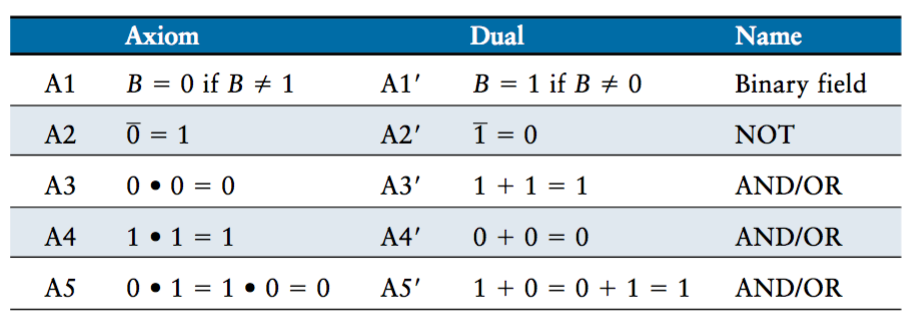
\includegraphics[scale=0.7]{pictures/booleanAlgAxiom.png}

  \subsection{Theorems of One Variable}
  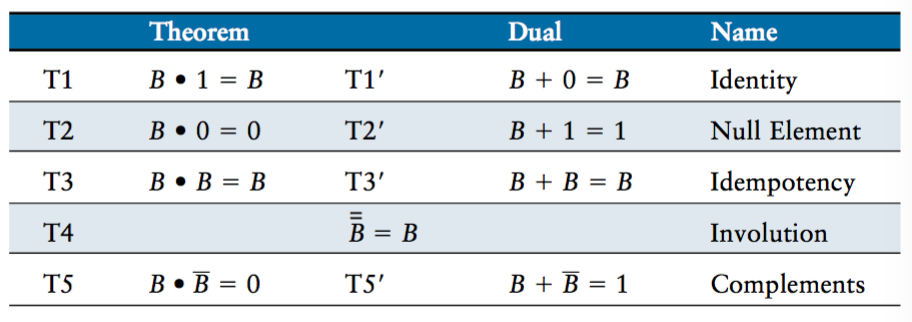
\includegraphics[scale=0.7]{pictures/booleanAlgOneVari.png}

  \subsection{Theorems of Several Variables}
  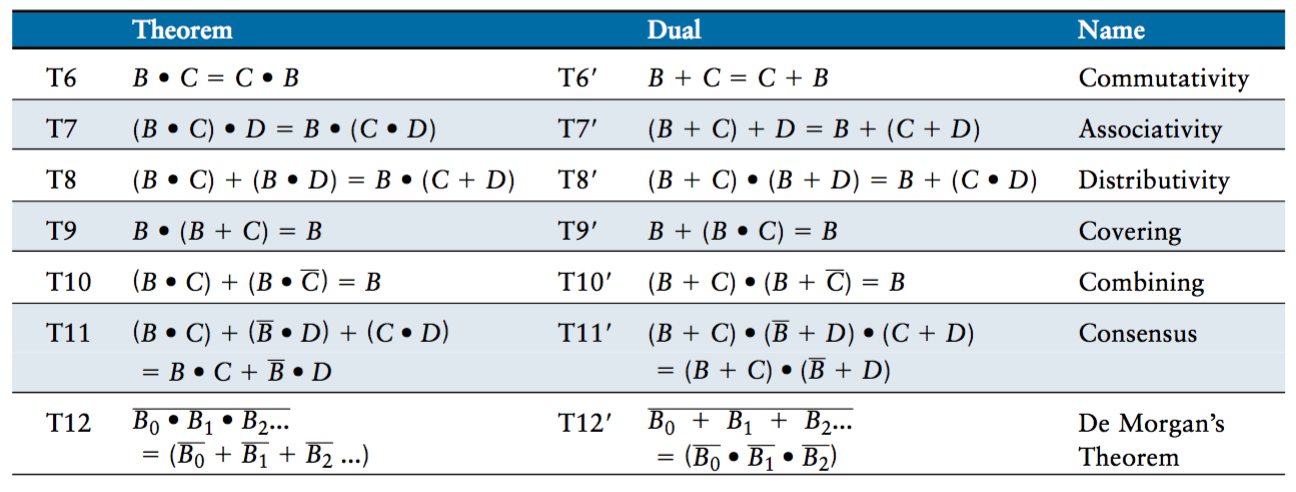
\includegraphics[scale=0.65]{pictures/booleanAlgMultVar.png}

  \newpage
  \section{From Logic to Gates}
  A \emph{schematic} is a diagram of a digital circuit showing the elements and the wires that connect them together. \\

  \textbf{Good Style in Circuit Drawing}:
  \begin{itemize}
    \item Assume all literals (variables and their negations) are available
    \item Rectilinear wires, dots when wires split
    \item Do not draw spaghetti wires for inputs; instead, write each literal as needed
  \end{itemize}

  \section{Multilevel Combinational Logic}
  Logic in sum-of-products form is called \emph{two-level logic} because it consists of literals connected to a level of AND gates connected to a level of OR gates. \\
  Designers often build circuits with more than two levels of logic gates.
  These multilevel combinational circuits may use less hardware than their two-level counterparts. \\
  Bubble pushing is especially helpful in analyzing and designing multilevel circuits.

  \subsection{Hardware Reduction}
  Some logic functions require an enormous amount of hardware when built using two-level logic.
  A notable example is the XOR function of multiple variables. \\
  A three-input XOR can be built out of a cascade of two-input XORs. \\
  Similarly, an eight-input XOR would require 128 eight-input AND gates and one 128-input OR gate for a two level-sum-of-products implementation. A much better option is to use a tree of two-input XOR gates. \\

  ``Best'' has many meanings: fewest gates, fastest, shortest design time, least cost, least power consumption. \\
  ``Best'' circuit in one technology is not necessarily the best in another.
  ANDs and ORs are used often, but in CMOS, NANDs and NORs are more efficient.

  \subsection{Bubble Pushing}
  CMOS circuits prefer NANDs and NORs over ANDs and ORs.
  However, reading the equation by inspection can be difficult. \\
  Bubble pushing is a helpful way to redraw these circuits so that the bubbles cancel out and the function can be more easily determined. \\
  Guidelines for bubble pushing:
  \begin{itemize}
    \item Begin at the output of the circuit and work toward the inputs.
    \item Push any bubbles on the final output back toward the inputs so that you can read an equation in terms of the output.
    \item Working backward, draw each gate in a form so that bubbles cancel. If the current gate has an input bubble, draw the preceding gate with an output bubble. If the current gate does not have an input bubble, draw the preceding gate without an output bubble.
  \end{itemize}

  \section{Combinational Building Blocks}
  Combinational logic is often grouped into larger building blocks to build more complex systems.
  This is an application of the principle of abstraction, hiding the unnecessary gate-level details to emphasize the function of the building block.

  \subsection{Multiplexers}
  \emph{Multiplexers}, also known as \emph{mux}, are among the most commonly used combinational circuits.
  They choose an output from among several possible inputs based on the value of a \emph{select} signal.

  \subsubsection{2:1 Multiplexer}
  \begin{wrapfigure}{r}{0.25\textwidth}
    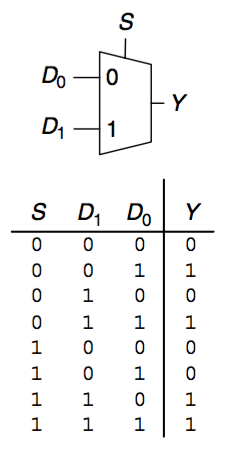
\includegraphics[width=0.25\textwidth]{pictures/2_1_mux.png}
  \end{wrapfigure}
  Image shows the schematic and truth table for a 2:1 multiplexer with two data inputs, $D_0$ and $D_1$, as select input, $S$, and one output, $Y$. \\
  The multiplexer chooses between the two data inputs based on the select:
  if $S = 0$, $Y = D_0$, and if $S = 1$, $Y = D_1$.  \\
  $S$ is also called a control signal because it controls what the multiplexer does. \\

  Multiplexers can be built from tristate buffers. \\
  The tristate enables are arranged such that, at all times, exactly one tristate buffer is active. \\
  When $S = 0$, tristate $T_0$ is enabled, allowing $D_0$ to flow to $Y$. \\
  When $S = 1$, tristate $T_1$ is enabled, allowing $D_1$ to flow to $Y$.

  \subsubsection{Wider Multiplexers}
  A 4:1 multiplexer has four data inputs and one output.
  Two select signals are needed to choose among the four data inputs.
  The 4:1 mux can be built using sum-of-products logic, tristates, or multiple 2:1 mux. \\

  The product terms enabling the tristates can be formed using AND gates and inverters.
  They can also be formed using a decoder. \\

  In general, an $N:1$ multiplexer needs $log_{2} N$ select lines.

  \subsubsection{Multiplexer Logic}
  Multiplexers can be used as \emph{lookup tables} to perform logic functions.
 \\
  In general, a $2^{N}$-input multiplexer can be programmed to perform any N-input logic functions by applying 0's and 1's to the appropriate data inputs. \\
  By changing the data inputs, the multiplexer can be reprogrammed to perform a different function.

  \subsection{Decoder}
  A decoder has $N$ inputs and $2^{N}$ outputs. \\
  It asserts exactly one of its outputs depending on the input combination.
  The outputs are called \emph{one-hot}, because exactly one is ``hot'' (HIGH) at a given time. \\

  Example of 2:4 decoder and its implementation: \\
  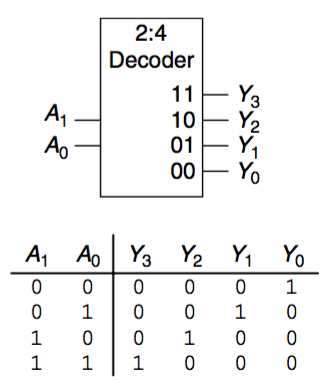
\includegraphics{pictures/2_4_decoder.png}
  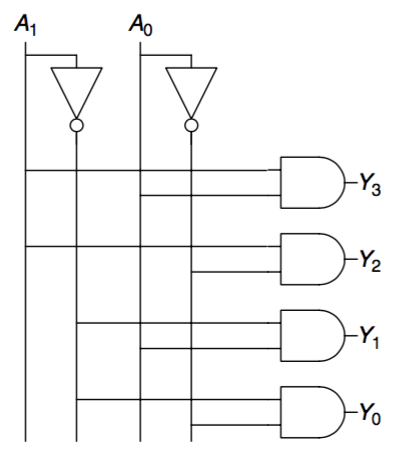
\includegraphics{pictures/2_4_decoder_implementation.png} \\

  \subsubsection{Decoder Logic}
  Decoders can be combined with OR gates to build logic functions. \\
  When using decoders to build logic, it is easiest to express functions as a truth table or in canonical sum-of-products form.
  A $N$-input function with $M$ 1's in the truth table can be built with an $N:2^{N}$ decoder and an $M$-input or gate attached to all of the minterms containing 1's in the truth table.

  \newpage
  \section{Summary So Far}
  A digital circuit is a module with discrete-valued inputs and outputs and a specification describing the function and timing of the module. \\

  The function of a combinational circuit can be given by a truth table or a Boolean equation. The Boolean equation for any truth table can be obtained systematically using sum-of-products or product-of-sums form. \\
  In sum-of-products form, the function is written as the sum (OR) of one or more implicants.
  Implicants are the product (AND) of literals.
  Literals are the true or complementary forms of the input variables.  \\

  Boolean equation can be simplified using the rules of Boolean algebra.
  In particular, they can be simplified into minimal sum-of-products form by combining implicants that differ only in the true and complementary forms of one of the literals: $PA + P\overline{A} = P$. \\

  Logic gates are connected to create combinational circuits that perform the desired function. \\
  Any functions in sum-of-products form can be built using two-level logic with the literals as inputs: NOT gates form the complementary literals, AND gates form the products, and OR gates form the sum. \\
  CMOS circuits favor NAND and NOR gates because these gates can be built directly from CMOS transistors without requiring extra NOT gates. \\
  When using NAND and NOR gates, bubble pushing is helpful to keep track of the inversions. \\

  Logic gates are combined to produce larger circuits such as multiplexers, decoders, and priority circuits. \\
  A multiplexer chooses one of the data inputs based on the select input. \\
  A decoder sets one of the outputs HIGH according to the input. \\
  A priority circuit produces an output indicating the highest priority input. \\

  The timing specification of a combinational circuit consists of the propagation and contamination delays through the circuit. \\
  These indicate the longest and shortest times between an input change and the consequent output change. \\
  Calculating the propagation delay of a circuit involves identifying the critical path through the circuit, then adding up the propagation delays of each element along that path.

  \newpage
  \section{Introduction to Sequential Logic Design}
  The output of sequential logic depend on both current and prior input values. \\
  Hence, sequential logic has memory.
  Sequential logic might explicitly remember certain previous inputs, or it might distill the prior inputs into a smaller amount of information called the \emph {state} of the system. \\
  The state of a digital sequential circuit is a set of bits called \emph{state variables} that contain all the information about the past necessary to explain the future behavior of the circuit.

  \subsection{Latches and Flip-Flops}
  The fundamental building block of memory is a \emph{bistable} element, an element with two stable states. \\
  An element with $N$ stable states conveys $\log_{2}N$ bits of information, so a bistable element stores one bit. \\
  The state of the cross-coupled inverters is contained in one binary state variable, $Q$.
  The value of $Q$ tells us everything about the past that is necessary to explain the future behavior of the circuit. \\
  Specifically, if $Q = 0$, it will remain 0 forever, and if $Q = 1$, it will remain 1 forever. \\
  The circuit does have another node, $\overline{Q}$, but $\overline{Q}$ does not contain any additional information because if $Q$ is known, $\overline{Q}$ is also known.
  $\overline{Q}$ is also an acceptable choice for the state variable. \\

  When power is first applied to a sequential circuit, the initial state is unknown and usually unpredictable.
  It may differ each time the circuit is turned on. \\

  Although the cross-coupled inverters can store a bit of information, they are not practical because the user has no inputs to control the states. \\
  However, other bistable elements, such as \emph{latches} and \emph{flip-flops}, provide inputs to control the value of the state variable.

  \blfootnote{$Y$ is commonly used for the output of combinational logic, $Q$ is commonly used for the output of sequential logic.}
  \newpage
  \subsubsection{SR Latch}
  \begin{wrapfigure}{r}{0.25\textwidth}
    \centering
    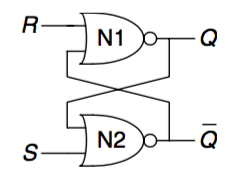
\includegraphics[width=0.25\textwidth]{pictures/srLatch.png}
  \end{wrapfigure}

  \emph{SR latch} is one of the simplest sequential circuit as it is composed of two cross-coupled NOR gates. \\
  The latch has two inputs, $S$ and $R$, and two outputs, $Q$ and $\overline{Q}$. \\
  The SR latch is similar to the cross-coupled inverters, but its state can be controlled through the $S$ and $R$ inputs, which \emph{set} and \emph{reset} the output $Q$. \\

  Consider the four possible combinations of $R$ and $S$:
  \begin{itemize}
    \item[\emph{Case I:}] $R = 1, S = 0$ \\
    N1 sees at least one TRUE input, $R$, so it produces a FALSE output on $Q$.
    N2 sees both $Q$ and $S$ FALSE, so it produces a TRUE output on $\overline{Q}$.
    \item[\emph{Case II:}] $R = 0, S = 1$ \\
    N1 receives inputs of 0 and $\overline{Q}$.
    Because we don't yet know $\overline{Q}$, we can't determine the output $Q$.
    N2 receives at least one TRUE input, $S$, so it produces a FALSE output on $\overline{Q}$.
    Now we can revisit N1, knowing that both inputs are FALSE, so the output $Q$ is TRUE.
    \item[\emph{Case III:}] $R = 1, S = 1$ \\
    N1 and N2 both set at least one TRUE input ($R$ or $S$), so each produces a FALSE output.
    Hence $Q$ and $\overline{Q}$ are both FALSE.
    \item[\emph{Case IV:}] $R = 0, S = 0$ \\
    N1 receives inputs of 0 and $\overline{Q}$.
    Because we don't yet know $\overline{Q}$, we can't determine the output.
    N2 receives inputs of 0 and $Q$.
    Because we don't yet know $Q$, we can't determine the output.
    Now we are stuck.
    This is reminiscent of the cross-coupled inverters.
    But we know that $Q$ must either be 0 or 1.
    So we can solve the problem by checking what happens in each of these sub-cases.
    \begin{itemize}
      \item[\emph{Sub-case a:}] $Q = 0$ \\
      Because $S$ and $Q$ are FALSE, N2 produces a TRUE output on $\overline{Q}$. Now N1 receives one TRUE input, $\overline{Q}$, so its output, $Q$, is FALSE.
      \item[\emph{Sub-case b:}] $Q = 1$ \\
      Because $Q$ is TRUE, N2 produces a FALSE output on $\overline{Q}$. Now N1 receives two FALSE inputs, $R$ and $\overline{Q}$, so its output, $Q$, is TRUE.
    \end{itemize}
  \end{itemize}

  Suppose $Q$ has some known prior value, $Q_{prev}$, before we enter Case IV. $Q_{prev}$ is either 0 or 1, and represents the state of the system.
  When $R$ and $S$ are 0, $Q$ will remember this old value, $Q_{prev}$, and $\overline{Q}$ will be its complement, $\overline{Q}_{prev}$.
  This circuit has memory. \\

  Like the cross-coupled inverters, the SR latch is a bistable element with one bit of state stored in $Q$.
  However, the state can be controlled through the $S$ and $R$ inputs. \\
  When $R$ is asserted, the state is reset to 0. \\
  When $S$ is asserted, the state is set to 1. \\
  When neither is asserted, the state retains its old value.

  \subsubsection{D Latch}
  The SR latch is awkward because it behaves strangely when both $S$ and $R$ are simultaneously asserted.
  Moreover, the $S$ and $R$ inputs conflate the issues of \emph{what} and \emph{when}.
  Asserting one of the inputs determines not only \emph{what} the state should be but also \emph{when} it should change. \\
  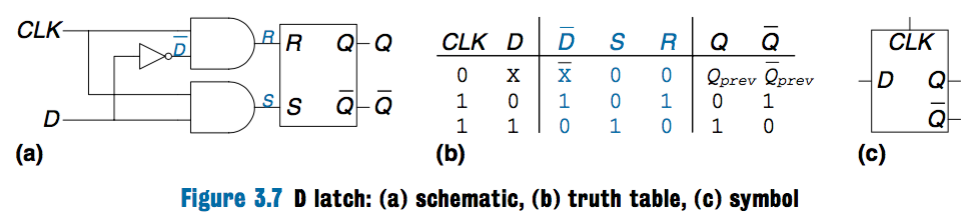
\includegraphics[width=1.0\textwidth]{pictures/dLatch.png}\\
  The D latch has two inputs.
  The \emph{data} input, $D$, controls what the next state should be.
  The \emph{clock} input, $CLK$, controls when the state should change. \\
  The clock controls when data flows through the latch. \\
  When $CLK = 1$, the latch is \emph{transparent}.
  The data at $D$ flows through to $Q$ as if the latch were just a buffer. \\
  When $CLK = 0$, the latch is \emph{opaque}.
  It blocks the new data from flowing through to $Q$, and $Q$ retains the old value. \\
  The D latch updates its state continuously $CLK = 1$.
  \newpage
  \subsubsection{D Flip-Flop}
  \begin{wrapfigure}{r}{0.3\textwidth}
    \centering
    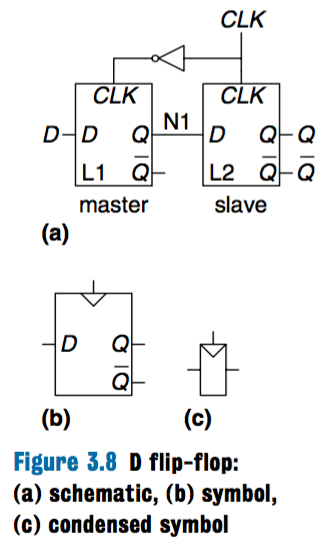
\includegraphics[width=0.3\textwidth]{pictures/dFlipFlop.png}
  \end{wrapfigure}
  A \emph{D flip-flop} can be built from two back-to-back D latches controlled by complementary clocks. \\
  The first latch, $L1$, is called the \emph{master}. \\
  The second latch, $L2$, is called the \emph{slave}. \\
  The node between them is named $N1$. \\
  A symbol for the D flip-flop is given in the figure (b). \\
  When the $\overline{Q}$ output is not needed, the symbol can be condensed as in figure (c). \\

  When $CLK = 0$, the master latch is transparent and the slave is opaque.
  The value at $D$ propagates through to $N1$. \\
  When $CLK = 1$, the master goes opaque and the slave becomes transparent.
  The value at $N1$ propagates through to $Q$, but $N1$ is cut off from $D$.
  Hence, the value at $D$ immediately before the clock rises from 0 too 1 gets copied to $Q$ immediately after the clock rises. \\
  At other times, $Q$ retains its old value, because there is always an opaque latch blocking the path between $D$ and $Q$.

  \begin{figure}[!ht]
  \centering
  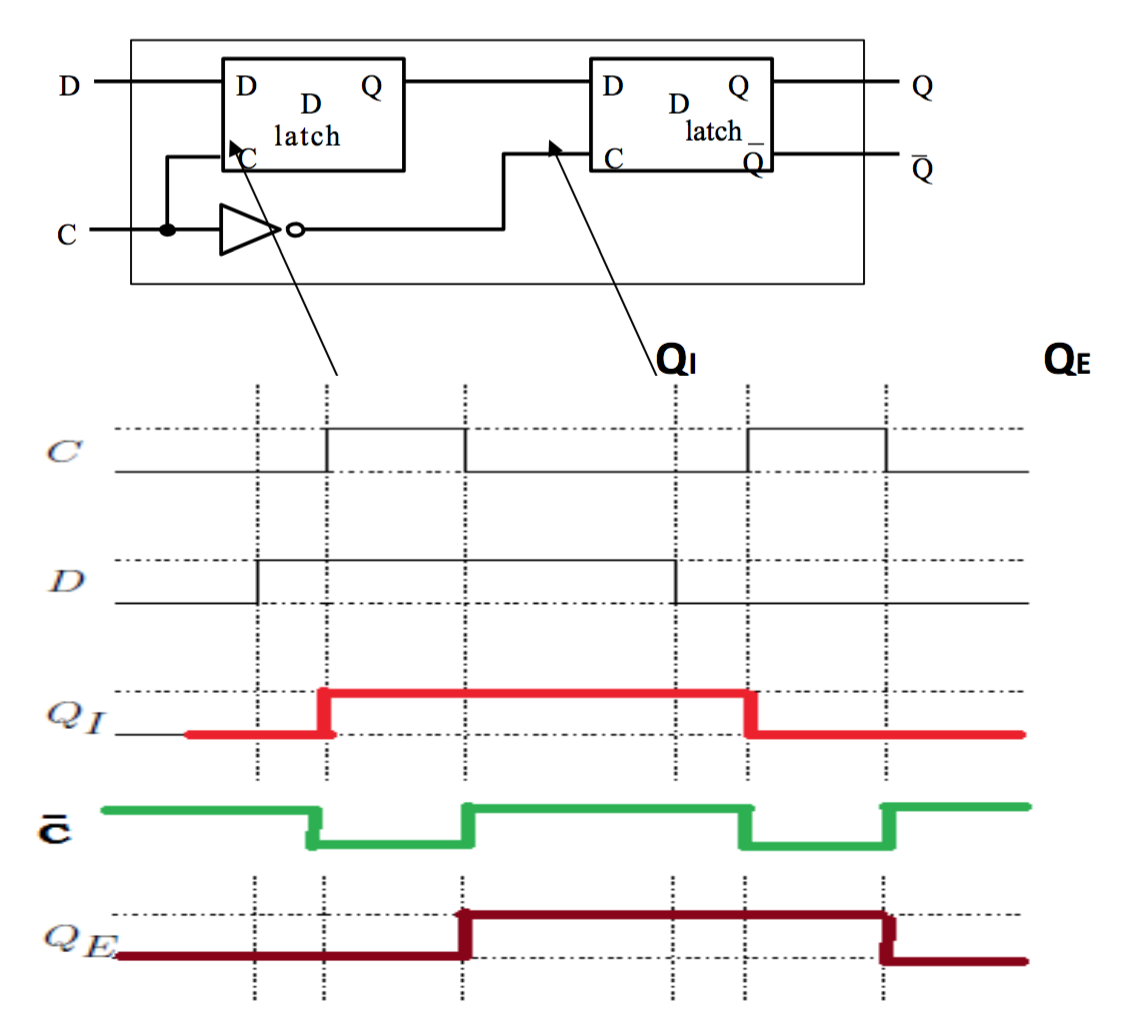
\includegraphics[width=0.55\textwidth]{pictures/dFlipFlopExample.png} \\
  \caption{A D flip-flop example.}
  \end{figure}
  A \emph{D flip-flop} copies $D$ to $Q$ on the rising edge of the clock, and remembers its state at all other times. \\

  A D flip-flop is also known as a \emph{master-slave flip-flop}, an \emph{edge-triggered flip-flop}, or a \emph{positive edge-triggered flip-flop}.

  \subsubsection{Register}
  A $N$-bit register is a bank of $N$ flip-flops that share a common $CLK$ input, so that all bits of the register are updated at the same time. \\
  Registers are the key building block of most sequential circuits. \\

  For a 32-bit architectures, a register would typically have 32 flip-flops in parallel (i.e. one for each bit). \\
  A \emph{register file} is a way of organizing registers. \\
  \includePicture{1.0}{pictures/registerFile.png}{A register file.} \label{registerFile} \\

  \textbf{Reading from a Register File} \\
  The values of all 32 registers go through two multiplexers. \\
  The first multiplexer determines which register value will be routed to the 1\textsuperscript{st} output. \\
  The second multiplexer determines which register value will be routed to the 2\textsuperscript{nd} output. \\
  It will take 5 select lines to uniquely identify each source register (when there are 32 registers).

  \textbf{Writing to a Register File} \\
  The address of the register $d$, is routed through a decoder which determines which D flip-flop to write to. \\
  When the $d^{\text{th}}$ decoder line and the \emph{RegWrite} line are both 1, they pass a 1 through the $d^{\text{th}}$ AND gate and raise the $C$ input of the $d^{\text{th}}$ D flip-flop to 1. \\
  The data will now be written to Register $\$d^{\text{th}}$.

  \section{Finite State Machines}
  Synchronous sequential circuits can be drawn in the forms called \emph{finite state machines (FSMs)}.
  The name comes from a circuit with $k$ registers can be in one of a finite number ($2^{k}$) of unique states. \\
  A FSM has $M$ inputs, $N$ outputs, and $k$ bits of state.
  It also receives a clock and, optionally, a reset signal. \\
  An FSM consists of two blocks of combinational logic, \emph{next state logic} and \emph{output logic}, and a register that stores the state.
  On each clock edge, the FSM advances to the next state, which was computed based on the current state and inputs. \\
  Finite state machines provides a systematic way to design synchronous sequential circuits given a functional specification.

  Two general classes of finite state machines, characterized by their functional specifications. \\
  In \emph{Moore machines}, the outputs depend only on the current state of the machine. \\
  In \emph{Mealy machines}, the outputs depend on both the current state and the current inputs.

  \begin{wrapfigure}{r}{0.4\textwidth}
    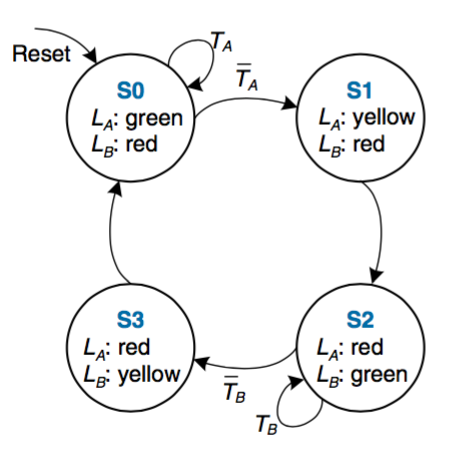
\includegraphics[width=0.4\textwidth]{pictures/stateTransistionDiagram.png}
  \end{wrapfigure}

  \subsection{State Transition Diagram}
  A \emph{state transition diagram} indicates all the possible states of the system and the transitions between these states. \\
  In a state transition diagram, circles represent states and arcs represent transitions betweens states. \\
  The transitions take place on the rising edge of the clock; the clock can hidden on the diagram because it is always present in a synchronous sequential circuit.
  In addition, the clock only controls when the transitions should occur, whereas the diagram indicates which transitions occur. \\
  If a state has multiple arcs leaving it, the arcs are labeled to show what input triggers each transition.
  In the image, when in state $S0$, the system will remain in that state if $T_{A}$ is TRUE and move to $S1$ if $T_{A}$ is FALSE. \\
  If a state has a single arc leaving it, that transition always occurs regardless of the inputs.
  In the image, when in state $S1$, the system will always move to $S2$.

  \subsection{State Transition Table}
  \includePicture{0.8}{pictures/stateTTableStateEncode.png}{Example Transition Table and its Encoding}
  A \emph{state transition table} indicates for each state and input, what the next state, $S'$, should be.
  If the next state does not depend on a particular input, the don't care symbol (X) is used. \\
  To build a real circuit, the states and outputs must be assigned \emph{binary encodings}.

  \subsection{State Encoding}
  If the state and output encodings were selected arbitrarily, a different choice would have resulted in a different circuit. \\
  Then how to determine the encoding that produces the circuit with the fewest logic gates or the shortest propagation delay?
  There is not simply method to find the best encoding. \\
  It is possible to choose a good encoding by inspection, so that related states share bits. \\

  An important decision in state encoding is the choice between binary encoding and one-hot encoding. \\
  With \emph{binary encoding}, each state is represented as a binary number.
  Because $K$ binary numbers can be represented by $\log_{2}K$ bits, a system with $K$ states only needs $\log_{2}K$ bits of state. \\

  In \emph{one-hot encoding},  a separate bit of state is used for each state.
  It is called one-hot because only one bit is ``hot'' or TRUE at any time.
  \begin{ex}
    A one-hot encoded FSM with three states would have state encodings of 001, 010, and 100.
  \end{ex}
  Each bit of state is stored in a flip-flop, so one-hot encoding requires more flip-flops than binary encoding.
  However, with one-hot encoding, the next-state and output logic is often simpler, so fewer gates are required. \\

  Another encoding is the \emph{one-cold} encoding, in which $K$ states are represented with $K$ bits, exactly one of which is FALSE.

  \subsection{FSM Review} \label{FSM_Review}
  Finite state machines are a powerful way to systematically design sequential circuits from a written specification. \\
  Procedure to design an FSM:
  \begin{enumerate}
    \item[>] Identify the inputs and outputs.
    \item[>] Sketch a state transition diagram.
    \item[>] For a Moore machine:
    \begin{enumerate}
      \item[-] Write a state transition table.
      \item[-] Write an output table.
    \end{enumerate}
    \item[>] For a Mealy machine:
    \begin{enumerate}
      \item[-] Write a combined state transition and output table.
    \end{enumerate}
    \item[>] Select state encodings---selection affects the hardware design.
    \item[>] Write Boolean equations for the next state and output logic.
    \item[>] Sketch the circuit schematics.
  \end{enumerate}

  \section{Summary So Far}
  In contrast to combinational logic, whose outputs depend solely on the current inputs, sequential logic outputs depend on both current and prior inputs.
  Sequential logic remembers information about prior inputs.
  This memory is called the state of the logic. \\

  Sequential circuits can be difficult to analyze and are easy to design incorrectly.
  An important element is the flip-flop, which receives a clock and an input, $D$, and produces an output, $Q$.
  The flip-flop copies $D$ to $Q$ on the rising edge of the clock and otherwise remembers the old state of $Q$.
  A group of flip-flops sharing a common clock is called a register.
  Flip-flops may also receive reset or enable control signals. \\

  Finite state machines are a powerful technique for designing sequential circuits. \\

  Synchronous sequential circuits have a timing specification including to clock-to-$Q$ propagation and contamination delay, $t_{pcq}$ and $t_{ccq}$, and the setup and hold times, $t_{setup}$ and $t_{hold}$. \\
  For correct operation, their inputs must be stable during an aperture time that starts a setup time before the rising edge of the clock and ends a hold time after the rising edge of the clock. \\

  The minimum cycle time, $T_{c}$, of the system is equal to the propagation delay, $t_{pd}$, through combinational logic plus $t_{pcq} + t_{setup}$ of the register. \\
  For correct operation, the contamination delay through the register and combinational logic must be greater than $t_{hold}$.
  Hold time does not affect the cycle time. \\

  Overall performance is measured in latency and throughput.
  The latency is the time required for a token to pass from start to end.
  The throughput is the number of tokens that the system can process per unit time.
  Parallelism improves the system throughput.

  \newpage
  \section{Multiplication}
  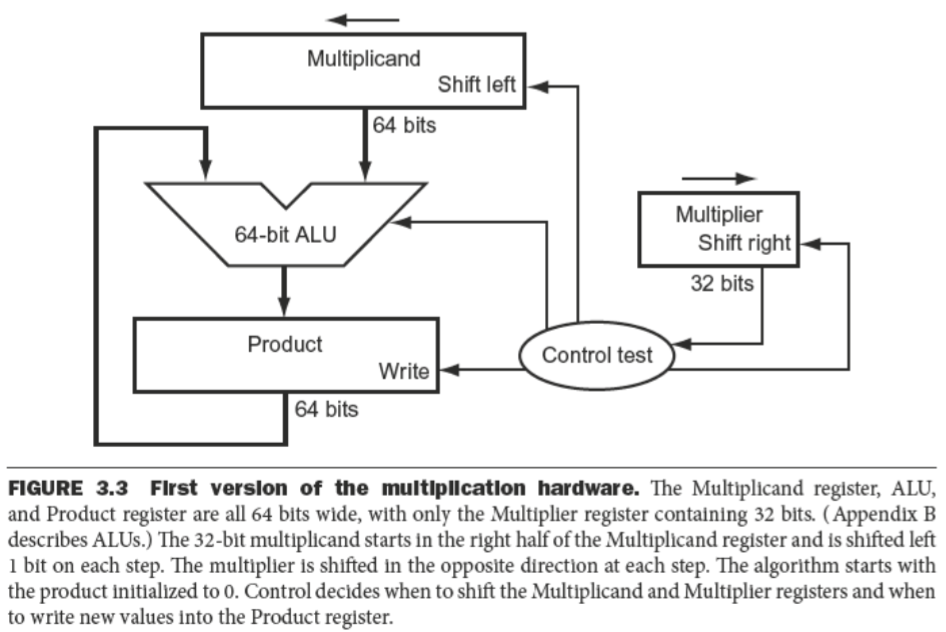
\includegraphics[width=1.0\textwidth]{pictures/multiplication.png} \\
  The first operand is called the \emph{multiplicand} and the second the \emph{multiplier}.
  The final result is called the \emph{product}. \\\
  Number of bits in the product is considerably larger than the number in either the multiplicand or the multiplier.
  If ignoring the sign bit, the length of the multiplication of an $n$-bit multiplicand and an $m$-bit multiplier is a product that is $n + m$ bits long.
  So $n + m$ bits are required to represent all possible products.

  \section{Floating Point}
  A number in scientific notation that has no leading 0s is called a \emph{normalized} number, which is the usual way to write it. \\
  \emph{Floating point} is computer arithmetic that represents numbers in which the binary point is not fixed. \\
  A standard scientific notation for reals in normalized form offers tree advantages:
  \begin{enumerate}
    \item It simplifies exchange of data that includes floating-point numbers.
    \item It simplifies the floating-point arithmetic algorithms to know that numbers will always be in this form.
    \item It increases the accuracy of the numbers that can be stored in a word, since the unnecessary leading 0s are replaced by real digits to the right of the binary point.
  \end{enumerate}

  \subsection{Floating-Point Representation}
  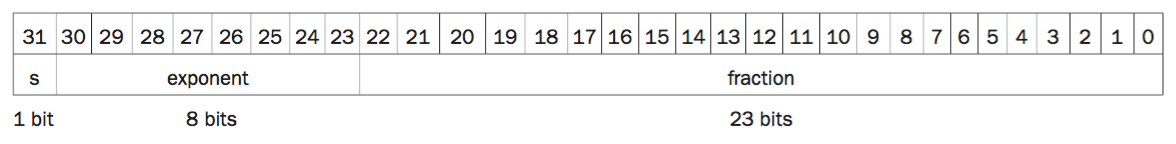
\includegraphics[width=1.0\textwidth]{pictures/mipsFloat.png} \\
  $s$ is the sign of the floating-point number (1 meaning negative).
  \emph{exponent} is the value of the 8-bit exponent field (including the sign of the exponent).
  \emph{fraction} is the 23-bit number. \\
  Generally, floating-point numbers are of the form: $$(-1)^{s} \times F \times 2^{E}$$
  F involves the value in the fraction field and E involves the value in the exponent field.

  \blfootnote{\emph{overflow}: positive exponent becomes too large to fit in the exponent field}
  \blfootnote{\emph{underflow}: negative exponent becomes too large to fit in the exponent field}

  A \emph{double precision} floating-point number is represented in two 32-bit words.
  The exponent is the value of the 11-bit exponent field.
  Fraction is the 52-bit number in the fraction field. \\
  \includePicture{0.85}{pictures/floatingPoints.png}{IEEE 754 encoding of floating-point numbers.}

  This is also known as the \emph{IEEE 754 floating-point standard}.
  This standard has greatly improved both the ease of porting floating-point programs and the quality of computer arithmetic. \\
  In IEEE 754, the leading 1-bit of normalized binary number is implicit, so the number is actually 24 bits long in single precision. \\

  For the fractional part, suppose we number the bits of the fraction from left to right $s1$, $s2$, $s3$, \dots, then the value is
  $$(-1)^{S} \times (1 + (s1 \times 2^{-1}) + (s2 \times 2^{-2}) + (s3 \times 2^{-3}) + (s4 \times 2^{-4}) + \dots) \times 2^{E}$$

  IEEE 754 uses a bias of 127 for single precision exponent. \\
  The exponent bias for double precision is 1023. \\
  So the value represented by a floating-point number is really
  $$(-1)^{S} \times (1 + \text{Fraction}) \times 2^{(\text{Exponent} - \text{Bias})}$$

  \subsection{Floating-Point Addition}
  \begin{itemize}
    \item[1.] Compare the exponents of the two numbers; shift the smaller number to the right until its exponent would match the larger exponent.
    \item[2.] Add the significants.
    \item[3.] Normalize the sum, either shifting right and incrementing the exponent or shifting left and decrementing the exponent.
    \item[>] Overflow or underflow? If yes, Exception. Otherwise, continue.
    \item[4.] Round the significant to the appropriate number of bits.
    \item[>] Still normalized? If no, then step 3. Otherwise, done.
  \end{itemize}
  \includePicture{0.7}{pictures/floatingAddition.png}{Arithmetic unit for floating-point addition.}

  \subsection{Floating-Point Multiplication}
  \begin{itemize}
    \item[1.] Add the biased exponents of the two numbers, subtracting the bias from the sum to get the new biased exponent.
    \item[2.] Multiply the significants.
    \item[3.] Normalize the product if necessary, shifting it right and incrementing the exponent.
    \item[>] Overflow or underflow? If yes, Exception. Otherwise, continue.
    \item[4.] Round the significant to the appropriate number of bits.
    \item[>] Still normalized? If no, then Step 3. Otherwise, continue.
    \item[5.] Set the sign of the product to positive if the signs of the original operands are the same; if they differ, make the sign negative.
  \end{itemize}

  \newpage
  \section{Introduction to the Processor}
  A subset of the core MIPS instruction set will be examined:
  \begin{enumerate} \label{instruction_classes}
    \item[>] The memory-reference instructions \emph{load word} (lw) and \emph{store word} (sw)
    \item[>] The arithmetic-logical instructions add, sub, AND, OR, and slt
    \item[>] The branch instructions \emph{branch equal} (beq) and \emph{jump} (j)
  \end{enumerate}
  To implement those instructions, the first two steps are identical:
  \begin{enumerate}
    \item Send the \emph{program counter} (PC) to the memory that contains the code and fetch the instruction from that memory.
    \item Read one or two registers, using fields of the instruction to select the registers to read. For the load word instruction, only need to read one register, but most other instructions require reading two registers.
  \end{enumerate}
  After the two steps, the required actions depend on the instruction class.
  For each of the three instructions classes (\ref{instruction_classes}), the actions are largely the same, independent of the exact instruction. \\
  The simplicity and regularity of the MIPS instruction set simplifies the implementation by making the execution of many of the instruction classes similar. \\

  All instruction classes, except jump, use the arithmetic-logical unit (ALU) after reading the registers.
  The memory-reference instructions use the ALU for an address calculation, the arithmetic-logical instructions for the operation execution, and branches for comparison. \\
  After using the ALU, the actions required to complete various instruction classes differ. \\
  A memory-reference instruction will need to access the memory either to read data for a load or write data for a store. \\
  An arithmetic-logical or load instruction must write the data from the ALU or memory back into a register. \\
  For a branch instruction, it may be required to change the next instruction address based on the comparison; otherwise, the PC should be incremented by 4 to get the address of the next instruction.

  \section{Building a Data-path}
  \includePicture{0.7}{pictures/readingFetchingInstruction.png}{A portion of the data-path used for fetching instructions and incrementing the program counter.}
  A \emph{data-path element} is a unit used to operate within a processor.
  In the MIPS implementation, the data-path element include the instruction and data memories, the register file, the ALU, and adders. \\
  To execute any instruction, start by fetching the instruction from memory.
  Then increment the program counter so that it points at the next instruction, 4 bytes later. \\
  Refer to the figure above for how the elements are combined, forming a data-path that fetches instructions and increments the PC. \\

  A \emph{R-type \emph{or} R-format} is an arithmetical-logical instruction since they perform. \\
  All R-format instructions read two registers, perform an ALU operation on the contents of the register, and write the result to a register. \\

  Through a register file, it contains the register state of the computer and the ALU needs to operate on the values read from the registers. \\
  R-format instructions have three register operands, to read two data words from the register file and write one data word into the register file for each instruction. \\
  For each data word to be read from the register, an input to the register file is needed that will carry the value that has been read from the registers. \\
  To write a data word, two inputs are needed: one to specify the register number to be written and one to supply the \emph{data} to be written into the register. \\
  The register file always outputs the contents of whatever register numbers are on the Read register inputs.
  However, writes are controlled by the write control signal, which must be asserted for a write to occur at the clock edge. \\

  Thus, we need a total of four inputs (three for register number and one for data) and two outputs (both for data).
  The register number inputs are 5 bits wide to specify one of 32 registers ($32 = 2^{5}$), whereas the data input and two data output buses are each 32 bits wide (each word is 32 bits).

  \subsection{R-Format ALU Operations}
  Two elements are needed to implement R-format ALU operations: register file (\ref{registerFile}) and the ALU. \\

  The register file contains all the registers and has two read ports and one write port.
  The register file outputs the contents of the registers corresponding to the Read register inputs on the outputs; no other control inputs are needed. \\
  Note that a register write must be explicitly indicated by asserting the write control signal, $RegWrite$.
  Writes are edge-triggered, so that all write inputs must be valid at the clock edge. \\

  The inputs carrying the register number to the register file are all 5 bites wide, whereas the lines carrying data values are 32 bits wide. \\
  The operation to be performed by the ALU is controlled with the ALU operation signal, which will be 4 bits wide.

  \subsection{Memory-Reference Operations}
  \includePicture{0.75}{pictures/elementsFormemoryReference.png}{Two units needed for loads and stores. In addition to the register file and ALU.}
  Consider $lw$ and $sw$ instructions.
  They compute a memory address by adding the base register to the 16-bit signed offset field contained in the instruction. \\
  If the instruction is a store, the value to be stored must also be read from the register file where it resides in the destination register. \\
  If the instruction is a load, the value read from memory must be written into the register file in the specified register. \\
  Thus, both register and the ALU are required in addition to more. \\

  We need a unit to \emph{sign-extend} the 16-bit offset field in the instruction to a 32-bit signed value, and a data memory unit to read from or write to.
  A \emph{sign-extend} is to increase the size of a data item by replicating the high-order sign bit of the original data item in the high-order bits of the larger, destination data item. \\
  The data memory must be written on store instructions; hence, data memory has read and write control signals, an address input, and an input for the data to be written into memory. \\
  Refer to figure above for the two units required.

  \subsection{Branch Operations}
  \includePicture{0.6}{pictures/branchInstruction.png}{Data-path for branch operations.}
  $beq$ instruction has three operands, two registers that are compared for equality, and a 16-bit offset used to compute the \emph{branch target address} relative to the branch instruction address. \\
  For this instruction, we need to compute the branch target address by adding the sign-extended offset field of the instruction to the PC.
  Note the two following details in the definition of branch instructions:
  \begin{itemize}
    \item The instruction set architecture specifies that the base for the branch address calculation is the address of the instruction following the branch.
    Since we compute $PC + 4$ (the address of the next instruction) in the instruction fetch data-path, it is easy to use this value as the base for computing the branch target address.
    \item The architecture also states that the offset field is shifted left 2 bits so that it is a word offset; this shift increases the effective range of the offset field by a factor of 4.
  \end{itemize}
  The offset field can be shifted by 2 to resolve the second complication. \\

  For computing the branch target address, we need to determine whether the next instruction is the instruction that follows sequentially or the instruction at the branch target address. \\
  When the operands are equal, the branch target address becomes the new PC, and it can be said that \emph{branch \emph{is} taken}. \\
  If the operands are not equal, the incremented PC should replace the current PC (just as for any other normal instruction); thus the \emph{branch \emph{is} not taken}.

  \blfootnote{\textbf{branch taken}: a branch where the branch condition is satisfied and the program counter (PC) becomes the branch target. All unconditional jumps are taken branches.}
  \blfootnote{\textbf{branch not taken}: a branch where the branch condition is false and the program counter (PC) becomes the address of the instruction that sequentially follows the branch.}

  Therefore, the branch data-path must do two operations: compute the branch target address and compare the register contents. \\
  To compute the branch target address, the branch data-path includes a sign extension unit and an adder. \\
  To perform the compare, a register file is needed to supply the two register operands.
  \newpage
  \section{Creating a Single Data-path}
  The simplest data-path will attempt to execute all instructions in one-clock cycle.
  No data-path resource can be used more than once per instruction, so any element needed more than once must be duplicated.
  So a memory for instructions separate from one for data is needed.
  Some of the functional units will need to be duplicated, many of the elements can be shared by different instruction flows. \\

  To share a data-path element between two different instruction classes, we may have to allow multiple connections to the input of an element, using a multiplexer and control signal to select among the multiple inputs.
  \newpage
  \section{A Full Data-Path}
  \begin{figure}[!htp]
    \centering
    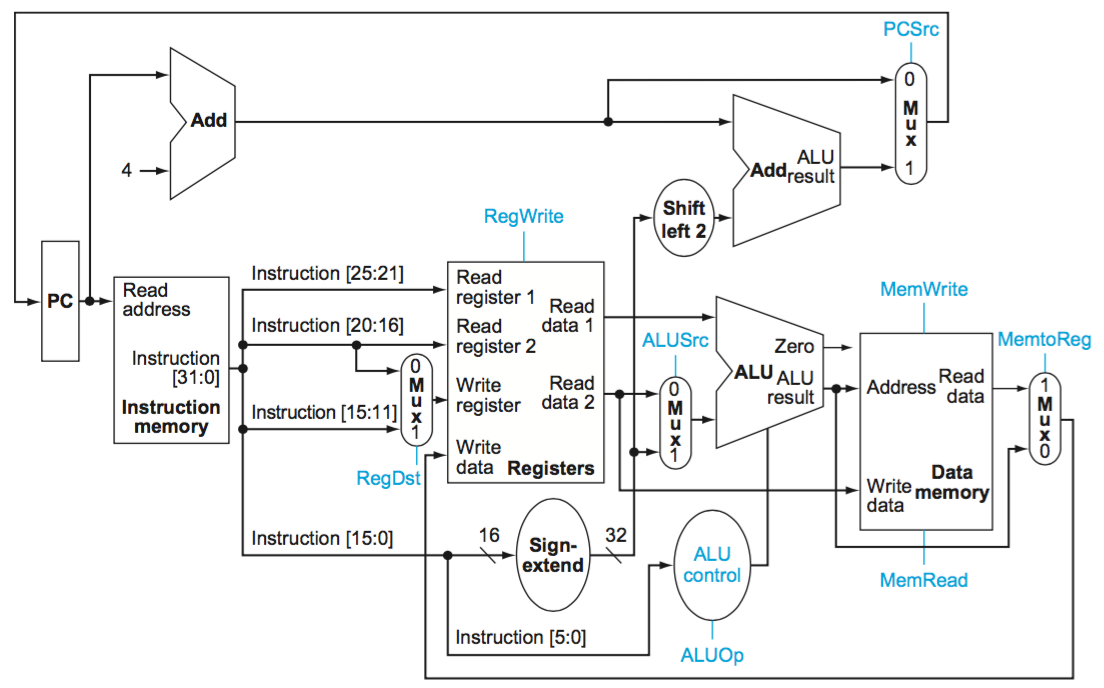
\includegraphics[angle=90, width=1.0\textwidth]{pictures/fullDataPath.png}
    \caption{Data-path with all necessary multiplexers and all control lines.}
    \label{fullDataPath}
  \end{figure}
  \newpage
  \section{A Simple Implementation Scheme}
  \subsection{The ALU Control}
  The MIPS ALU defined in ``Computer Organization and Design'' Appendix B defines the 6 following combinations of four control inputs:
  \begin{center}
  \begin{tabular} {c | c}
    ALU Control Lines & Function          \\ \hline
    0000              & AND               \\ \hline
    0001              & OR                \\ \hline
    0010              & add               \\ \hline
    0110              & subtract          \\ \hline
    0111              & set on less than  \\ \hline
    1100              & NOR               \\ \hline
  \end{tabular}
  \end{center}
  The ALU will need to perform one of the first five functions depending on the instruction class.
  NOR will be covered later. \\
  For load and store word instructions, ALU is used to compute the memory address by addition. \\
  For R-type instructions, ALU needs to perform AND, OR, subtract, add, or set on less than, depending on the value of the 6-bit function field in the low-order bits of the instruction. \\
  For branch equal, the ALU must perform a subtraction. \\

  In many instances, we do not care about the values of some of the \emph{inputs}, and because we wish to keep the tables compact, we also include \emph{don't-care terms}.
  A don't-care term in this truth table (represented by an X in an input column) indicates that the output does not depend on the value of the input corresponding to that column.

  \subsection{Designing the Main Control Unit}
  The three instruction classes (R-Type, load and store, and branch) use two different instruction formats; jump instructions use another format
  \begin{itemize}
    \item R-format instructions have an opcode of 0.
    They have three register operands: rs, rt, and rd.
    Fields rs and rt are sources, and rd is the destination.
    The ALU function is in the funct field and is decoded by the ALU control design.
    The shamt field is used only for shifts.
    \item Instruction format for load (opcode=35) and store (opcode=43) instructions.
    The register rs is the base register that is added to the 16-bit address field to form the memory address.
    For load, rt is the destination register for the loaded value.
    For stores, rt is the source register whose value should be stored in memory.
    \item Instruction format for branch equal (opcode=4).
    The registers rs and rt are the source registers that are compared for equality.
    The 16-bit address field is sign-extended, shifted, and added to the PC+4 to compute the branch target address
  \end{itemize}

  The general format of instructions are
  \begin{itemize}
    \item The op field, opcode, is always contained in bits 31:26.
    \item The two registers to be read are always specified by the rs and rt fields, at positions 25:21 and 20:16.
    This is true for the R-type instructions, branch equal, and store.
    \item The base register for load and store instruction is always in bit position 25:21 (rs).
    \item The 16-bit offset for branch equal, load, and store is always in positions 15:0.
    \item The destination register is in one of two places.
    For a load, it is in bit positions 20:16 (rt), while for an R-type instruction it is in bit positions 15:11 (rd).
    Thus, a multiplexer is added to select which field of the instruction is used to indicate the register number to be written.
  \end{itemize}

  The control unit can set all but one of the control signals based solely on the opcode field of the instruction.
  The PCSrc control line is the exception; that control line should be asserted if the instruction is branch on equal (a decision that the control unit can make) \emph{and} the Zero output of the ALU, which is used for equality comparison, is asserted. \\

  \textbf{Outputs for Control Unit} \\
  The output from the control unit are the control lines that:
  \begin{enumerate}
    \item Signal when memory should be write enabled (1-3)
    \item Signal when data lines a multiplexer show forward on (4-7)
    \item Signal which function the ALU should perform (8)
  \end{enumerate}
  \begin{tabular}{c || l | p{5cm} | l}
  & Signal/Outputs & If Signal == 1 & If Signal == 0 \\ \hline \hline
  1. & \emph{MemWrite} & Write to Data Memory & No effect \\ \hline
  2. & \emph{MemRead} & Memory read memory & No effect \\ \hline
  3. & \emph{RegWrite} & Write data to Register File & NO effect \\ \hline
  4. & \emph{MemtoReg} & Use data from Data Memory & Use ALUResult \\ \hline
  5. & \emph{Branch} & Use PCBranch result for PC & No branch; use PC + 4 \\ \hline
  6. & \emph{RegDst} & Use 15:11 field for write address (rd used) & Use 20:16 field (rt used) \\ \hline
  7. & \emph{ALUSrc} & Use immediate field from Instr & Use Register File \\ \hline
  8. & \emph{ALUControl\textsubscript{2:0}} &
  \multicolumn{2}{l}{Specify the ALU operation: add, sub, and, or}
  \end{tabular} \\

  The settings of the control lines is completely determined by the opcode fields of the instruction.
  \begin{multicols}{4}
  \begin{enumerate}
    \item R-Format
    \begin{enumerate}
      \item[RegDst] 1
      \item[ALUSrc] 0
      \item[MemtoReg] 0
      \item[RegWrite] 1
      \item[MemRead] 0
      \item[MemWrite] 0
      \item[Branch] 0
      \item[ALUOp1] 1
      \item[ALUOp0] 0
    \end{enumerate}
    \item lw
    \begin{enumerate}
      \item[RegDst] 0
      \item[ALUSrc] 1
      \item[MemtoReg] 1
      \item[RegWrite] 1
      \item[MemRead] 1
      \item[MemWrite] 0
      \item[Branch] 0
      \item[ALUOp1] 0
      \item[ALUOp0] 0
    \end{enumerate}
    \item sw
    \begin{enumerate}
      \item[RegDst] X
      \item[ALUSrc] 1
      \item[MemtoReg] X
      \item[RegWrite] 0
      \item[MemRead] 0
      \item[MemWrite] 1
      \item[Branch] 0
      \item[ALUOp1] 0
      \item[ALUOp0] 0
    \end{enumerate}
    \item beq
    \begin{enumerate}
      \item[RegDst] X
      \item[ALUSrc] 0
      \item[MemtoReg] X
      \item[RegWrite] 0
      \item[MemRead] 0
      \item[MemWrite] 0
      \item[Branch] 1
      \item[ALUOp1] 0
      \item[ALUOp0] 1
    \end{enumerate}
  \end{enumerate}
  \end{multicols}

  \textbf{ALU Decoder}
  How the main decoder signals the ALU decoder: \\
  \begin{tabular} {l | l}
  ALUOp\textsubscript{1:0} & Meaning \\ \hline \hline
  00 & Add \\ \hline
  01 & Subtract \\ \hline
  10 & Look at Funct \\ \hline
  11 & Not Used \\ \hline
  \end{tabular} \\

  The inputs (ALUOp\textsubscript{1:0} and Funct) and the output (ALUControl\textsubscript{2:0}): \\
  \begin{tabular}{l | l | l}
  ALUOp\textsubscript{1:0} & Funct Field & ALUControl\textsubscript{2:0} \\ \hline \hline
  00 & X & 010 (Add) \\ \hline
  X1 & X & 110 (Subtract) \\ \hline
  1X & 100000 (add) & 010 (Add) \\ \hline
  1X & 100010 (sub) & 110 (Subtract) \\ \hline
  1X & 100100 (and) & 000 (And) \\ \hline
  1X & 100101 (or) & 001 (Or)
  \end{tabular}

  \subsection{Procedure of Executing the Load Instruction}
  \begin{enumerate}
    \item[1] \emph{Fetch} the instruction, say \emph{lw \$2, 4(\$1)}
    \begin{enumerate}
      \item Start at the program counter (PC) to get the address of the next instruction
      \item Go the the \emph{Instruction Memory} to get next instruction
    \end{enumerate}
    \item[2a] Get the value stored in the \emph{Register File} at location \emph{\$1}
    \begin{enumerate}
      \item Specify the address (00001) at input A1 of the \emph{Register File}
      \item The data will appear at output RD1 of the \emph{Register File}
    \end{enumerate}
    \item[2b] \emph{Sign extend} the \emph{offset}
    \begin{enumerate}
      \item The offset, 4, is specified in the instruction
      \item Convert the offset from a 16-bit signed integer to a 32-bit signed integer by sign extending it
    \end{enumerate}
    \item[2c] Calculate the memory address of the data
    \begin{enumerate}
      \item Send the base address and the offset to inputs \emph{SrcA} and \emph{SrcB} of the \emph{Arithmetic Logic Unit} (ALU)
      \item Signal the \emph{ALU} to add the inputs with control signal \emph{ALUControl}
      \item The sum will appear at \emph{ALUResult}
    \end{enumerate}
    \item[2d] Read the data stored at this address
    \begin{enumerate}
      \item Send the memory address to the \emph{Data Memory}
      \item The data stored at that address will appear at output \emph{RD}
    \end{enumerate}
    \item[2e] Write the data into the \emph{Register File} at location \emph{\$2}
    \begin{enumerate}
      \item Send the \emph{ReadData} back to the \emph{Register File}
      \item Send the address (00010) to the \emph{Register File}
      \item Signal the \emph{Register File} to store the data (\emph{RegWrite}) at input \emph{WD3}
    \end{enumerate}
  \end{enumerate}

  \subsection{Why a Single-Cycle Implementation Is Not Used Today}
  It is inefficient because the clock cycle must have the same length for every instruction in single-cycle design. \\
  The longest possible path in the processor determines the clock cycle, which is the load instruction.
  It uses instruction memory, the register file, the ALU, the data memory, and the register file in series. \\

  There's significant drawback for using single-cycle design with a fixed clock cycle; but it may be considered acceptable for a small instruction set. \\
  It does not scale well when adding more complex instructions. \\
  It is not possible to improve the worst-case cycle time in a single-cycle design even if there are techniques to improve the common-case cycle time. \\

  Thus, we use pipelining to improve the efficiency and throughput.
  Pipelining improves efficiency by executing multiple instructions simultaneously.

  \newpage
  \section{An Overview of Pipelining}
  \emph{Pipelining} is an implementation technique in which multiple instructions are overlapped in execution. \\
  The idea to that all steps---called \emph{stages} in pipelining---are operating concurrently.
  As long as each stage has separate resources, the tasks can be pipelined. \\

  For pipelining MIPS instructions, each instruction classically takes five steps (stages):
  \begin{itemize}
    \item[1.] Fetch instruction from memory
    \item[2.] Read registers while decoding the instruction. The regular format of MIPS instructions allow reading and decoding to occur simultaneously.
    \item[3.] Execute the operation or calculate an address.
    \item[4.] Access an operand in data memory
    \item[5.] Write the result into a register
  \end{itemize}
  If the stages are perfectly balanced, then the time between instructions on the pipelined processor---assuming ideal condition---is equal to
  $$\text{Time between instructions}_\text{pipelined} = \frac{\text{Time between instruction}_\text{non-pipelined}}{\text{Number of pipe stages}}$$
  Under ideal condition and a large number of instruction, the performance is increased is approximately equal to the number of pipe stages. \\

  Pipelining improves performance \emph{increasing instruction throughput, as opposed to decreasing the execution time of an individual instruction}, but instruction throughput is the important metric because real programs execute billions of instruction.

  \subsection{Designing Instruction Sets for Pipelining}
  All MIPS instructions are the same length, which makes it easier to fetch instructions in the first pipeline stage and to decode them in the second stage. \\
  MIPS has only a few instruction formats, with the source register fields being located in the same place in each instruction. \\
  Thus, the second stage can begin reading the register file at the same time that the hardware is determining what type of instruction was fetched.
  If not for the symmetry in instruction formats, stage 2 would need to be split resulting in 6 pipeline stages (longer pipelines are not desired). \\
  In addition, memory operands only appear in loads or stores in MIPS.
  Which means we can use the execute stage to calculate the memory address and then access memory in the following stage.

  \subsection{Pipeline Hazards}
  Situations when the next instruction cannot execute in the following clock cycle are called \emph{hazards}.

  \subsubsection{Structural Hazard}
  A \emph{structural hazard} means the hardware cannot support the combination of instructions that we want to execute in the same clock cycle.

  \subsubsection{Data Hazard}
  A \emph{pipeline data hazard}, a form of \emph{data hazard}, occurs when the pipeline must be stalled because one step must wait for another to complete. \\
  In other words, a planned instruction cannot execute in the proper clock cycle because data that is needed to execute the instruction is not yet available. \\

  \emph{Forwarding}, also called \emph{bypassing}, is a method of solving a data hazard by retrieving the missing data element from internal buffers rather than waiting for it to arrive from programmer-visible register or memory. \\
  Forwarding paths are valid only if the destination stage is later in the time than the source stage. \\
  In other words, there cannot be a valid forwarding path from the output of the memory access stage in the first instruction to the input of the execution stage of the following, since that would mean going backward in time. \\

  A \emph{load-use data hazard} is a specific form of data hazard in which the data being loaded by a load instruction has not yet become available when it is needed by another instruction. \\
  A \emph{pipeline stall}, also called a \emph{bubble}, is a stall initiated in order to resolve a hazard.

  \subsubsection{Control Hazard}
  A \emph{control hazard}, also called \emph{branch hazard}, arises from the need to make a decision based on the results of one instruction while others are executing. \\
  This hazard comes from branch instructions as the pipeline cannot know the next possible instructions after fetching a branch instruction. \\
  Two ways to resolve control hazards:
  \begin{enumerate}
    \item \textbf{Stall} \\
      Stall immediately after a branch instruction is fetched, waiting until the pipeline determines the outcome of the branch and knows that instruction address to fetch from. \\
      If the branch cannot be resolved in the second stage, the cost of stalling is too high for most computes to use as it causes a even larger slowdown.
    \item \textbf{Predict} \\
      Computers use \emph{prediction} to handle branches.
      One approach is to predict always that branch will not be taken; when right,  the pipeline proceeds at full speed. \\
      If branch is taken, the pipeline stalls.
  \end{enumerate}

  A more sophisticated version of \emph{branch instruction} would have some branches predicted as taken and some as not taken. \\
  In programming, at the bottom of loops are branches that jump back to the top of the loop.
  Those branches are likely to be taken and they branch backwards, so it can be predicted as taken for branches that jump to an earlier address. \\
  \emph{Dynamic hardware predictors} make their guesses depending on the behavior of each branch and may change predictions for a branch over the life of a program.
  One approach is keeping a history for each branch as taken or not taken, and then using recent past history to predict the future. \\
  If prediction goes wrong, the pipeline control must ensure instructions following a wrongly guessed branch have no effect and must restart the pipeline from the proper branch address. \\

  A third approach to resolve control hazard is called \emph{delayed decision}, that's actually used in MIPS architecture.
  The delayed branch always execute the next sequential instruction, with the branch taking place after that one instruction delay.
  The assembler can automatically arrange the instructions to get the branch behavior desired by the programmer; it is hidden from the MIPS programmer.
  MIPS software places an instruction immediately after the delayed branch instruction that is not affected by the branch, and a taken branch changes the address of the instruction that follows this safe instruction. \\
  Delayed branches are useful when branches are short.
  Processors do not use a delayed branch of more than one cycle.
  For longer branch delays, hardware-based branch prediction is usually used.

  \subsection{Pipeline Overview Summary}
  Pipelining is a technique that exploits \emph{parallelism} among the instruction in a sequential instruction stream.
  Its substantial advantage is that it is fundamentally invisible to the programmer. \\
  Pipelining increases the number of simultaneously executing instructions and the rate at which instructions are started and completed.
  However, it does not reduce the time it takes to complete an individual instruction also called the \emph{latency}.
  \emph{Latency} in pipelining is the number of stages in a pipeline or the number of stages between two instruction during execution. \\
  Pipelining improves instruction \emph{throughput} rather than individual instruction \emph{execution time} or \emph{latency}.

  \section{Pipelined Datapath and Control}
  In a five-stage pipeline, up to five instructions will be in execution during any single clock cycle. \\
  The datapath can be separated into five pieces:
  \begin{enumerate}
    \item \textbf{IF}: Instruction fetch
    \item \textbf{ID}: Instruction decode and register file read
    \item \textbf{EX}: Execution or address calculation
    \item \textbf{MEM}: Data memory access
    \item \textbf{WB}: Write back
  \end{enumerate}
  For the register file and data memory units are split in two phases: write in the first half and read in the second half.

  \subsection{Pipelined Control}
  Only need to set the control values during each pipeline stage to specify control for the pipeline.
  Each control line is associated with a component active in only a single pipeline stage, thus the lines can be divided into five stages according to the pipeline stage.
  \begin{enumerate}
    \item \emph{Instruction fetch}:
    The control signals to read instruction memory and to write the PC are always asserted, so there is nothing special to control in this stage
    \item \emph{Instruction decode/register file read}:
    The same thing happens at every clock cycle, so there are not optional control lines to set.
    \item \emph{Execution/address calculation}:
    The signals to be set are \emph{RegDst}, \emph{ALUOp}, and \emph{ALUSrc}.
    The signals select the Result register, the ALU operation, and either Read data 2 or a sign-extended immediate for the ALU.
    \item \emph{Memory access}:
    The control lines set in this stage are \emph{Branch}, \emph{MemRead}, and \emph{MemWrite}.
    The branch equal, load, and store instructions set these signals respectively.
    Note that \emph{PCSrc} selects the next sequential address unless control asserts Branch and the ALU result was 0.
    \item \emph{Write back}:
    The two control lines are \emph{MemtoReg}, which decides between sending the ALU result or the memory value to the register file, and \emph{RegWrite}, which writes the chosen value.
  \end{enumerate}
  Implementing control means setting the nine control lines to these values in each stage for each instruction.
  The simple approach is to extend the pipeline registers to include control information. \\
  The control lines start with the \emph{EX} stage, so the control information can be created during instruction decode.

  \section{Data Hazards: Forwarding versus Stalling}
  The write is in the first half of the clock and the read is in the second half when a register is read and written in the same clock cycle.
  Thus, the read delivers what is written; this is a common implementation for register files. \\

  If the data is needed at the beginning of the EX stage, the data can be \emph{forwarded} as soon as it is available to any units that need it before the data is available in register file. \\
  For now, the only challenge of forwarding is to make the data available in an operation in the EX stage, which may either be an ALU operation or an effective address calculation.
  The two pairs of hazard conditions are:
  \begin{enumerate}
    \item[1a] EX/MEM.RegisterRd = ID/EX.RegisterRs
    \item[1b] EX/MEM.RegisterRd = ID/EX.RegisterRt
    \item[2a] MEM/WB.RegisterRd = ID/EX.RegisterRs
    \item[2b] MEM/WB.RegisterRd = ID/EX.RegisterRs
  \end{enumerate}

  \begin{ex}
    Suppose we have the following instructions sequence
    \begin{verbatim}
      sub $2,  $1, $3
      and $12, $2, $5
      or  $13, $6, $2
    \end{verbatim}
    Then sub-and is a type 1a hazard (EX/MEM.RegisterRd = ID/EX.RegisterRs)
    Whereas sub-or is a type 2b hazard (MEM/WB.RegisterRd = ID/EX.RegisterRs)
  \end{ex}
  This forwarding may not always work because some instructions do not write registers;
  sometimes it would forward when it shouldn't. \\
  A simple solution is to check if \emph{RegWrite} signal will be active: examining the WB control field of the pipelining register during the EX and MEM stages determines whether \emph{RegWrite} is asserted. \\
  Note that MIPS require every use of \$0 as an operand must yield an operand value of 0.
  Thus, need to avoid forwarding a possible non-zero value of \$0 in the event that \$0 is used as the destination.
  Thus, the conditions above work if EX/MEM.RegisterRd $\not =$ 0 and MEM/WB.RegisterRd $\not =$ 0.

  A new hardware, called \emph{Forwarding Unit} is added in the EX stage to expand the multiplexers into the ALU unit such that it can take in the forwarded data.
  \begin{center}
  \begin{tabular}{l | l | p{9cm}}
    Mux Control & Source & Explanation \\ \hline \hline
    ForwardA = 00 & ID/EX   & The first ALU operand comes from the register file \\ \hline
    ForwardA = 10 & EX/MEM  & The first ALU operand is forwarded from the prior ALU result. \\ \hline
    ForwardA = 01 & MEM/WB  & The first ALU is forwarded from data memory or an earlier ALU result \\ \hline
    ForwardB = 00 & ID/EX   & The second ALU operand comes from the register file \\ \hline
    ForwardB = 10 & EX/MEM  & The second ALU operand is forwarded from the prior ALU result. \\ \hline
    ForwardB = 01 & MEM/WB  & The second ALU is forwarded from data memory or an earlier ALU result \\ \hline
  \end{tabular}
  \end{center}
  Note that the EX/MEM.RegisterRd field is the register destination for either an ALU instruction (which comes from the Rd field of the instruction) or a load (which comes from the Rt field).
  \begin{enumerate}
    \item \emph{EX Hazard}
\begin{verbatim}
if (EX/MEM.RegWrite
and (EX/MEM.RegisterRd != 0)
and (EX/MEM.RegisterRd = ID/EX.RegisterRs))   ForwardA = 10

if (EX/MEM.RegWrite
and (EX/MEM.RegisterRd != 0)
and (EX/MEM.RegisterRd = ID/EX.RegisterRt))   ForwardB = 10
\end{verbatim}
    \item \emph{MEM Hazard}
\begin{verbatim}
if (MEM/WB.RegWrite
and (MEM/WB.RegisterRd != 0)
and not(EX/MEM.RegWrite and (EX/MEM.RegisterRd != 0)
      and (EX/MEM.RegisterRd != ID/EX.RegisterRs))
and (MEM/WB.RegisterRd = ID/EX.RegisterRs))   ForwardA = 01

if (MEM/WB.RegWrite
and (MEM/WB.RegisterRd != 0)
and not(EX/MEM.RegWrite and (EX/MEM.RegisterRd != 0)
      and (EX/MEM.RegisterRd != ID/EX.RegisterRt))
and (MEM/WB.RegisterRd = ID/EX.RegisterRt))   ForwardB = 01
\end{verbatim}
  \end{enumerate}

  \subsection{Data Hazards and Stalls}
  A particular case when forwarding does not work is when an instruction tries to read a register following a load instruction that writes the same register. \\
  In addition to a forwarding unit, we need a \emph{hazard detection unit} such that it can stall the pipeline.
  It is to operate during the ID stage so that it can insert the stall between the load and its use.
  \begin{verbatim}
  if (ID/EX.MemRead and
      ((ID/EX.RegisterRt = IF/ID.RegisterRs) or
        (ID/EX.RegisterRt = IF/ID.RegisterRt)))
        stall the pipeline
  \end{verbatim}
  The first line tests to see if the instruction is a load: the only instruction that reads data memory is a load.
  The next two lines check to see if the destination register field of the load in the EX stage matches either source register of the instruction in the ID stage. \\

  If the instruction in the ID stage is stalled, then the instruction in the IF stage must also be stalled;
  otherwise, we would lose the fetch instruction.
  So we execute instructions that have no effects: \emph{nops}.
  ``nop'' is an instruction that does no operation to change state.
  This way, the appropriate instructions can be stalled while depended instructions execute. \\

  By setting all nine control signals to 0 in the EX, MEM, and WB stages will create a ``do nothing'' or nop instruction. \\
  When the hazard is identified in the ID stage, a bubble can be inserted into the pipeline by changing the EX, MEM, and WB control fields of the ID/EX pipeline register to 0.
  No registers or memories are written if the control values are all 0. \\

  \begin{figure}[!ht]
  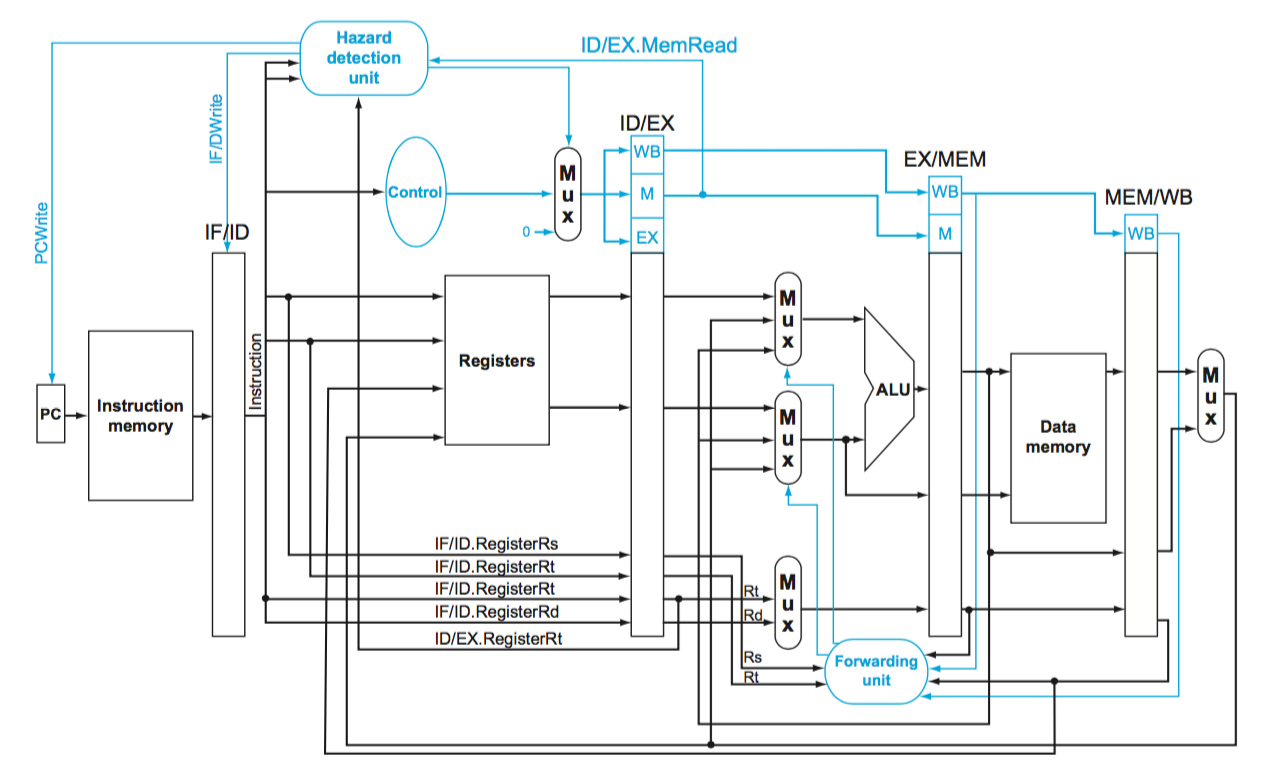
\includegraphics[width=1.0\textwidth]{pictures/hazardAndForwardingUnits.png}
  \caption{Implementation of Stalling and Forwarding}
  \end{figure}

  The \emph{hazard detection unit} controls the the writing of the PC and IF/ID registers plus the multiplexer that chooses between the real control values and all 0s. \\
  The unit stalls and deasserts the control fields if the load-use hazard test is true.

  \section{Control Hazards} % 4.8 in P+H
  An instruction must be fetched at every clock cycle to sustain the pipeline, the decision to branch does not occur until the MEM pipeline stage.
  This delay in determining the proper instruction to fetch is a \emph{control hazard} or \emph{branch hazard}. \\
  There are two schemes for resolving control hazards and one optimization to improve these schemes.
  \subsection{Assume Branch Not Taken}
  Stalling until the branch is complete is slow.
  An improvement is to \textbf{predict} that the branch will not be taken and thus continue execution down the sequential instruction stream. \\
  If branch is taken, the instructions that are being fetched and decoded must be discarded;
  execution continues at the branch target. \\
  If branches are not taken half the time, and if it costs little to discard the instructions, this method of optimization halves the cost of control hazards. \\

  To discard instructions, the original control values are changed to 0s, akin to stall a load-use data hazard. \\
  Note that all three instructions in the IF, ID, and EX stages need to be changed when the branch reaches the MEM stage;
  whereas only the controls in TD stage are changed to 0 and let them percolate through the pipeline. \\
  To discard instructions, the instructions in the IF, ID, and EX stages must be \textbf{flushed}.

  \subsection{Reducing the Delay of Branches}
  Another improvement is to reduce the cost of the taken branch.
  If branch execution is moved to an earlier stage in the pipeline, instead of MEM stage, then fewer instructions need to be flushed. \\
  Many branches rely only on simple tests that do not require a full ALU operation, it can be done with at most a few gates.
  If a more complex branch decision is needed, a separate instruction that uses an ALU is required. \\

  Moving the branch decision up requires two actions to occur earlier, and their respective complications:
  \begin{enumerate}
    \item Computing the branch target address
    \begin{itemize}
      \item The PC value and the immediate field are available in the IF/ID register.
      \item The branch adder can be moved from the EX stage to the ID stage.
      \item Note that the branch target address calculation will be performed for all instructions, but it will only be used when needed.
    \end{itemize}
    \item Evaluating the branch decision
    \begin{itemize}
      \item Moving the branch test to the ID stage implies additional forwarding and hazard detection hardware, since a branch dependent on a result still in the pipeline must work properly with this optimization.
      \item During ID: must decode the instruction, decide whether a bypass to the equality unit is required, and complete the comparison to set the PC if it is a branch instruction.
      \item A new forwarding logic is required for the equality test unit in ID. \\
      Bypassed source operands of a branch can come from either the ALU/MEM or MEM/WB pipeline latches.
      \item A data hazard can occur and a stall is needed if the values in a branch comparison are produced later in time.
    \end{itemize}
  \end{enumerate}
  The improvement of moving the branch execution to the ID stage is that the penalty of a branch is reduced to only one instruction if the branch is taken (the one being fetched in IF stage). \\
  To flush instructions in the IF stage, a control line named \emph{IF.Flush} zeros the instruction field of the IF/ID pipeline register. \\
  Clearing the register transforms the fetched instruction into a \textbf{nop}, an instruction that has no action and changes no state.

  \subsection{Dynamic Branch Prediction}
  Assuming a branch is not taken is a form of \emph{branch prediction}.
  It is probably adequate for a simple five-stage pipeline, and possibly coupled with compiler-based prediction.
  With more complex pipelines, the branch penalty increases when measured in clock cycles and it increases in terms of instructions lost.
  A simple static prediction scheme will waste too much performance in complex pipelines. \\

  \emph{Dynamic branch prediction} is to look up the address of the instruction to see if a branch was taken the last time this instruction was executed, and if so, to begin fetching new instructions from the same place as the last time. \\
  One implementation is a \emph{branch prediction buffer} and \emph{branch history table}.
  The buffer is a small memory indexed by the lower portion of the address of the branch instruction.
  This memory contains a bit that says whether the branch was recently taken or not. \\

  It is possible that the prediction is correct; another branch instruction could have used the same lower-order address bits. \\
  However, predicting is a hint that we hope is correct, so fetching begins in the predicted direction.
  Thus, it does not affect the correctness of the predictions. \\
  In the event that the hint is wrong, the incorrectly predicted instructions are deleted, the prediction bit is inverted and stored back. and the proper sequence is fetched and executed. \\

  A shortcoming of a 1-bit prediction scheme is that: even if a branch is almost always taken (ex. loop), the prediction can wrong twice, rather than once, when it's not taken. \\

  To remedy the weakness of poor accuracy of 1-bit prediction schemes, 2-bit prediction schemes are often used.
  A prediction must be wrong twice before it is changed in a 2-bit scheme. \\

  A branch prediction buffer can be implemented as a small special buffer accessed with the instruction address during the IF pipe stage. \\
  If the instruction is predicted as taken, fetching begins from the target as soon as the PC is known. \\
  Otherwise, sequential fetching and executing continue. \\
  If the prediction is wrong, the prediction bits are changed. \\

  \textbf{Elaboration}: \\
  A delayed branch always executes the following instruction, but the second instruction following the branch will be affected by the branch.
  Compilers and assemblers try to place an instruction that always executes after the branch in the \emph{branch delay slot}. \\

  \textbf{Elaboration}: \\
  A branch predictor tells whether or not a branch is taken, but still requires the calculation of the branch target.
  The calculation takes one cycle, which means that taken branches have a 1-cycle penalty. \\
  The penalty can be resolved by delayed branches or through a \emph{branch target buffer}.
  A branch target buffer is a structure that caches the destination PC or destination instruction for a branch.
  It is usually organized as a cache with tags, thus more costly than a simple prediction buffer.\\

  The 2-bit dynamic prediction scheme uses only information about a particular branch.
  However, using information about both a local branch, and the global behavior of recently executed branches together yields greater prediction accuracy for the same number of prediction bits.
  This is a \emph{correlating predictor}. \\
  A typical correlating predictor have two 2-bit predictors for each branch, with the choice between predictors made based on whether the last executed branch was taken or not.
  Thus, the global branch behavior can be thought as an adding additional index bits for the prediction lookup. \\

  A recent innovation in branch predicting is the use of tournament predictors. \\
  A \emph{tournament predictor} uses multiple predictors, tracking, for each branch, which predictor yields the best results.
  A typical one might contain two predictions for each branch index: one based on local information and the other based on global branch behavior. \\
  A selector would choose which predictor to use for any given prediction.
  The selector can operate similarly to a 1- or 2-bit predictor, favoring whichever of the two has been more accurate.

  \begin{figure}
  \centering
  \caption{The final datapath and control}
  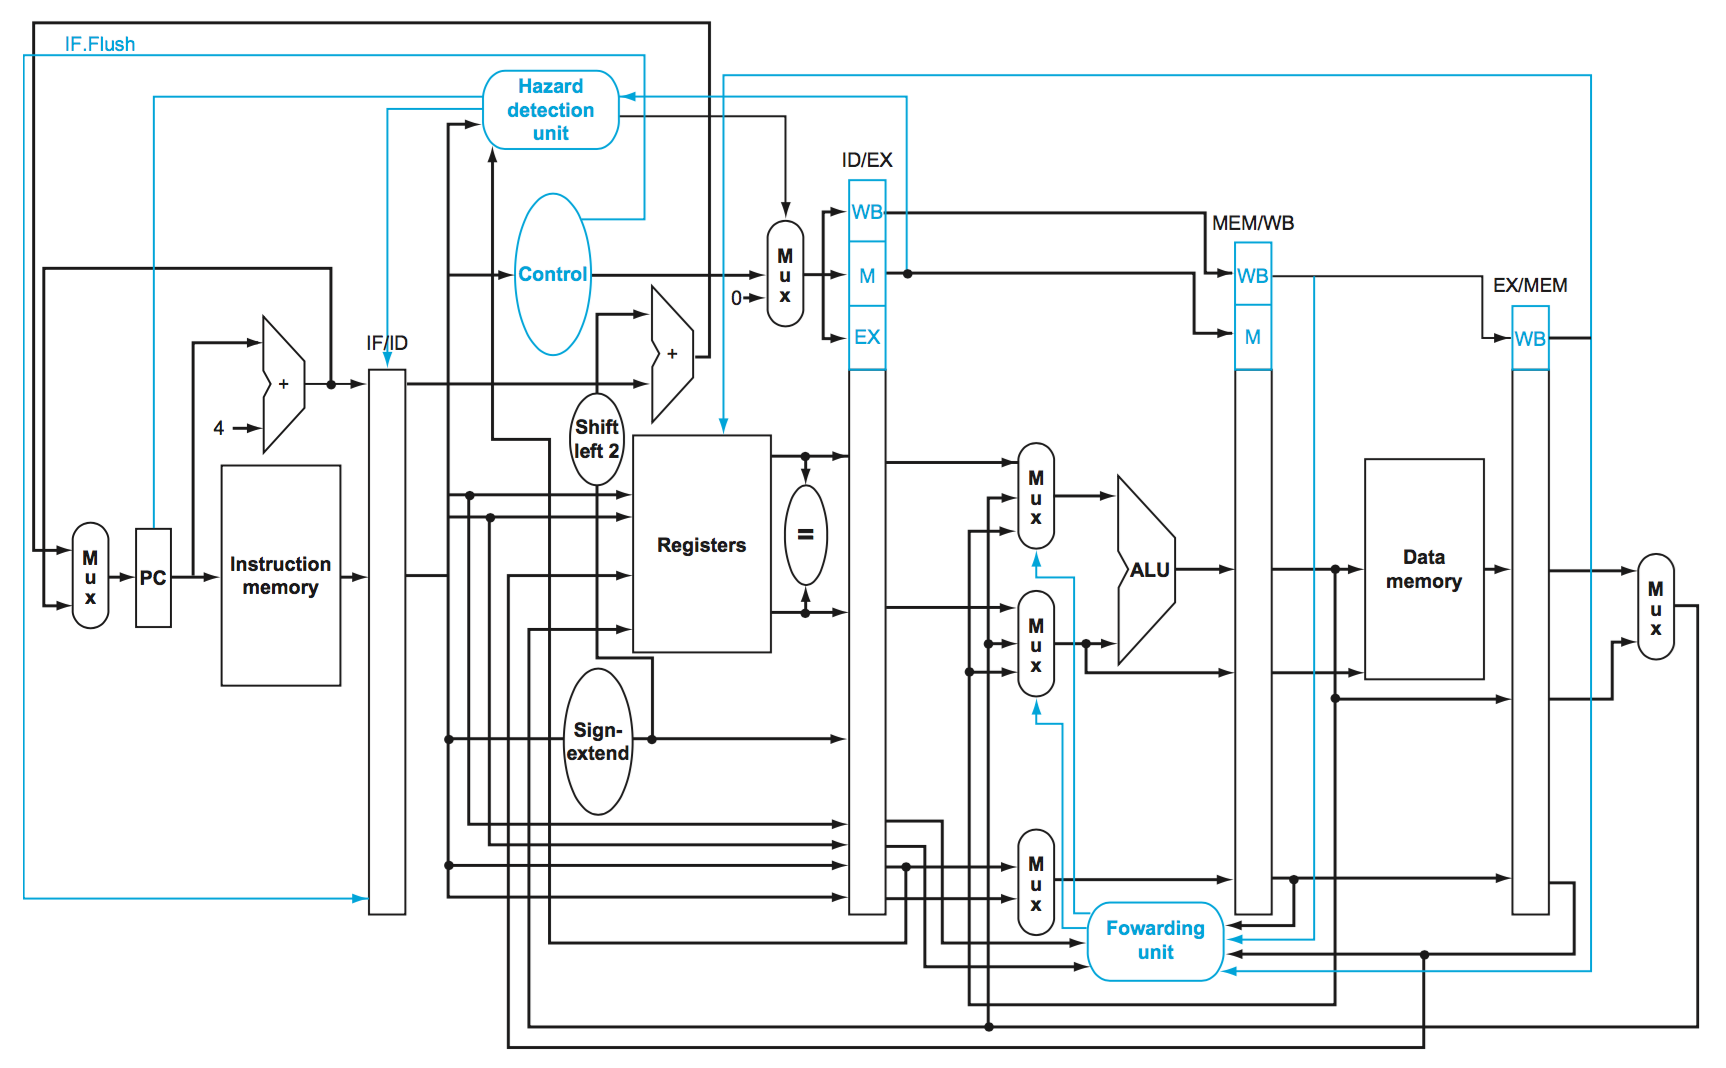
\includegraphics[width=1.0\textwidth]{pictures/finalPipelineDataPath.png}
  \end{figure}

  \section{Exceptions}
  Control is the most challenging aspect of processor design: it is both the hardest part to get right and the hardest part to make fast.
  One of the hardest parts of control is implementing \emph{exceptions} and \emph{interrupts}. \\
  An \emph{exception}, also called \emph{interrupt}, is an unscheduled event that disrupts program execution; used to detect overflows.
  An \emph{interrupt} is an exception that comes from outside of the processor.
  Initially created to handle unexpected events from within the processor, like arithmetic overflow. \\

  Detecting exceptional conditions and taking the appropriate action is often on the critical timing path of a processor, which determines the clock cycle time and thus performance. \\
  Without proper attention to exceptions during design of the control unit, attempts to add exceptions to a complicated implementation can significantly reduce performance, as well as complicate the task of getting the correct design.

  \subsection{How Exceptions Are Handled in the MIPS Architecture}
  The basic action that the processor must perform when an exception occurs is to save the address of the offending instruction in the \emph{exception program counter} (EPC) and then transfer control to the operating system at some specified address. \\

  The operating system (OS) can then take the appropriate action, which may involve providing some service to the user program, taking some predefined action in response to an overflow, or stopping the execution of the program and reporting an error. \\
  After performing the correct action is required due to the exception, the OS can terminate the program or may continue its execution, using the EPC to determine where to restart the execution of the program. \\

  For the OS to handle an exception, it must know the reason and the instruction that cause it. \\
  Two main methods to communicate the reason for an exception:
  \begin{enumerate}
    \item Include a status register (called the \emph{Cause Register}), which holds a field that indicates the reason for the exception.
    \item Use \emph{vectored interrupts}. In a vectored interrupt, the address to which control is transferred is determined by the cause of the exception. \\
    Ex. Type: undefined instruction; Vector address: 8000 0000\textsubscript{hex}
  \end{enumerate}

  The OS knows the reason for the exception by the address at which it is initiated.
  The addresses are separated by 32 bytes or eight instructions, and the OS must record the reason for the exception and may perform some limited processing in this sequence. \\
  When the exception is not vectored, a single entry point for all exceptions can be used, and the OS decodes the status register to find the cause. \\

  Two additional registers must be added to the MIPS implementation we have so far:
  \begin{itemize}
    \item[\emph{EPC}] A 32-bit register used to hold the address of the affected instruction. \\
    Such a register is needed even when exceptions are vectored.
    \item[\emph{Cause}] A register used to record the cause of the exception.
    In the MIPS architecture, this register is 32 bits, although some bits are unused.
  \end{itemize}

  \subsection{Exceptions in a Pipelined Implementation}
  A pipelined implementation treats exceptions as another form of control hazard.
  We will use the same mechanism used for taken branches, but this time the exception causes the deasserting of control lines. \\

  When dealing with branch mis-predict, the instruction in the IF stage is flushed by turning it into a \emph{nop}. \\
  To flush instructions in the ID stage, we use the multiplexer already in the ID stage that zeros control signals for stalls.
  A new control signal, called \emph{ID.Flush}, is ORed with the stall signal from the hazard detection unit to flush during ID. \\
  To flush instruction in the EX stage, a new signal called \emph{EX.Flush} is used to cause new multiplexers zero the control lines. \\
  Then we start fetching instructions from location 8000 0180\textsubscript{hex}, which is the MIPS exception address, we simply add an additional input to the PC multiplexer to send the address to the PC.

  \begin{figure}[!ht]
    \center{
      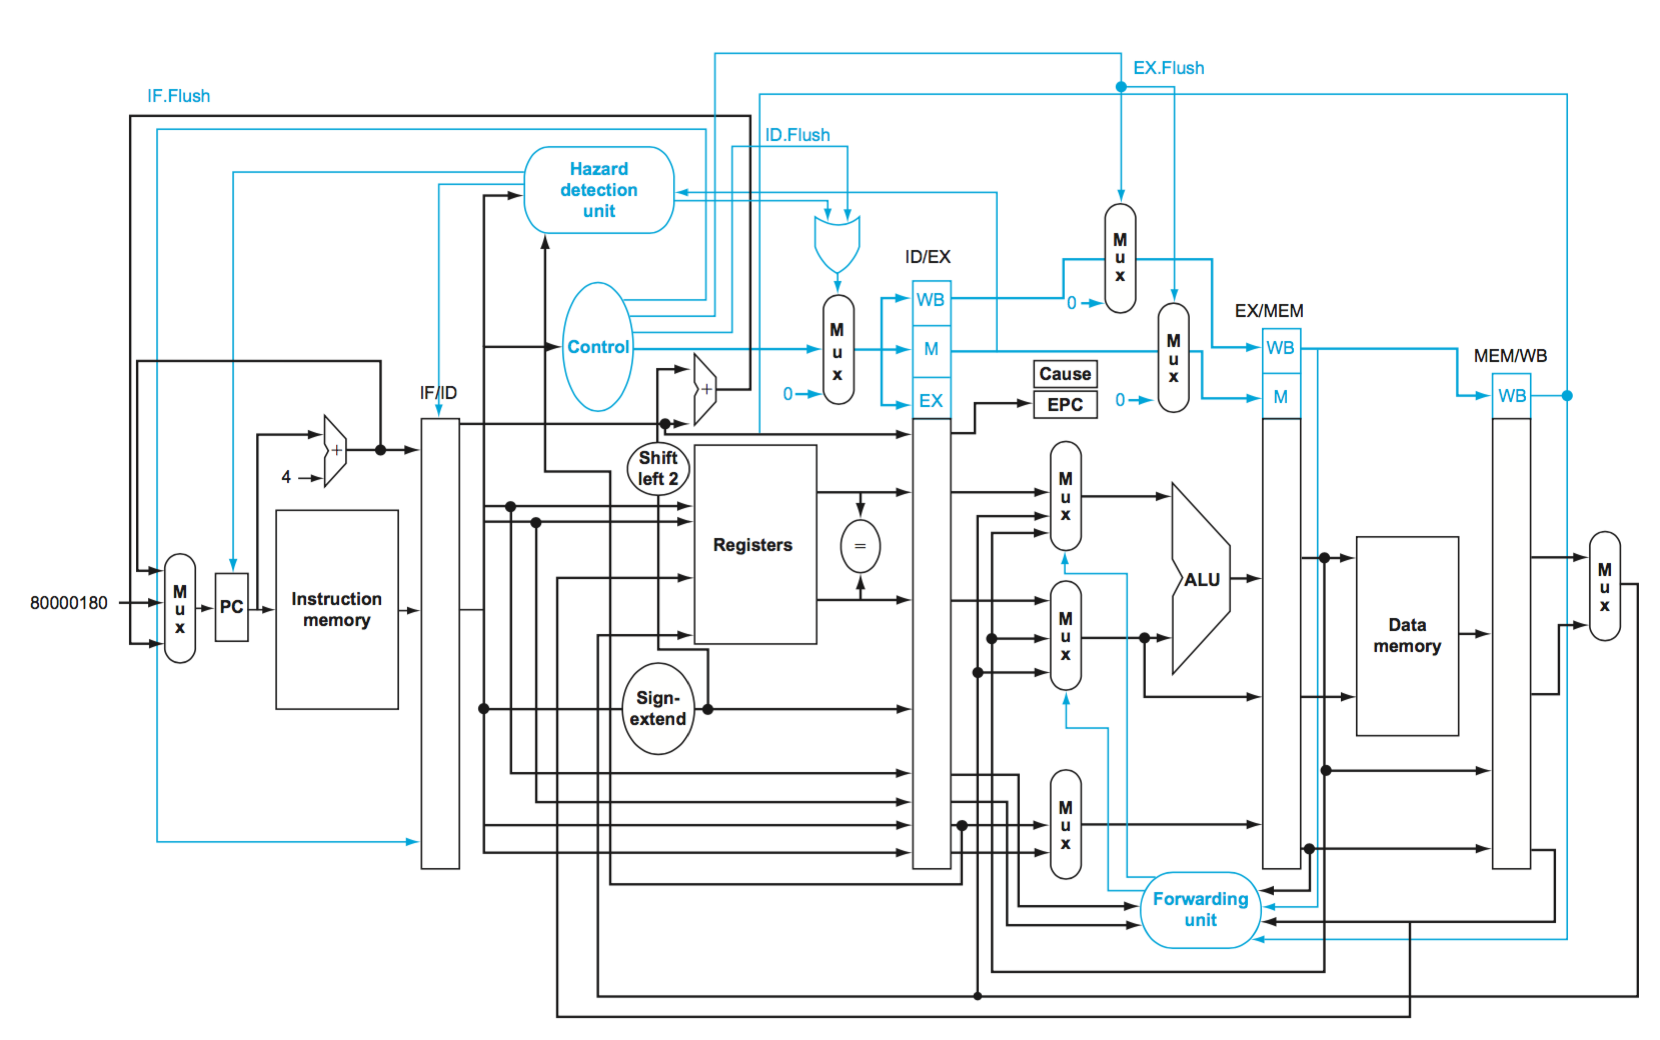
\includegraphics[width=1.0\textwidth]{pictures/datapathWithExceptions.png}
      \caption{The datapath with controls to handle exceptions}
    }
  \end{figure}

  Many exceptions require that we eventually complete the instruction that caused the exception as if it executed normally.
  The easiest way to do this is to flush the instruction and restart it from the beginning after the exception is handled. \\

  The final step is to save the address of the offending instruction in the \emph{exception program counter} (EPC).
  In reality, we save the address + 4, so the exception handling the software routine must subtract 4 from the saved value. \\

  Multiple exceptions can occur simultaneously in a single clock cycle.
  The solution is to prioritize the exceptions so that it is easy to determine which is serviced first.
  In most MIPS implementations, the hardware sorts exception so that the earliest instruction is interrupted. \\
  I/O device requests and hardware malfunctions are not associated with a specific instruction, so that implementation has some flexibility as to when to interrupt the pipeline. \\

  The EPC (exception program counter) captures the address of the interrupted instructions, and the MIPS Cause Register records all possible exceptions in a clock cycle, so the exception software must match the exception to the instruction.
  An important clue is knowing in which pipeline stage a type of exception can occur. \\
  Exceptions are collected in the Cause Register in a pending exception field so that the hardware can interrupt based on later exceptions, once the earliest one has been serviced.

  \subsection{Hardware/Software Interface}
  The hardware and the OS must work together so that exceptions behave as expected. \\

  The hardware contract is normally to stop the offending instruction in midstream, let all prior instructions complete, flush all following instructions, set a register to show the cause of the exception, save the address of the offending instruction, and then jump to a prearranged address. \\

  The OS contract is to look at the cause of the exception and act appropriately. \\
  For an undefined instruction, hardware failure, or arithmetic overflow exception, the operating system typically terminates the program and returns an indicator of the reason. \\
  For an I/O device request or an OS service call, the system saves the state of the program, performs the desired task, and, at some point in the future, restores the program to continue execution.
  We often choose to run another task before resuming the task that requested the I/O, since that task may often not be able to proceed until the I/O is complete. \\

  Exceptions are why the ability to save and restore the state of any task is critical. \\

  The difficulty of always associating the correct exception with the correct instruction in pipelined computers has led some computer designers to relax this requirement in noncritical cases.
  Such processors are said to have \emph{imprecise interrupts} or \emph{imprecise exceptions},
  which are interrupts/exceptions that are not associated with the exact instruction that was the cause. \\
  MIPS and the vast majority of computers today support \emph{precise interrupts} or \emph{precise exceptions}, which are interrupts/exceptions that are associated with the correct instruction.

  \newpage
  \section{Introduction to Large and Fast: Exploiting Memory Hierarchy}
  The \emph{principle of locality} states that programs access a relatively small portion of their address space at any instant of time. \\
  There are two different types of locality:
  \begin{enumerate}
    \item \textbf{Temporal Locality} (locality in time): if an item is referenced, it will tend to be referenced again soon.
    \item \textbf{Spatial Locality} (locality in space): if an item is referenced, items whose addresses are close by will tend to be referenced soon.
  \end{enumerate}
  Locality in programs arises from simple and natural program structures.
  For example, most programs contain loops, so instructions and data are likely to be accessed repeatedly, showing high amounts of temporal locality.
  In addition, those instructions are normally accessed sequentially, programs also show high spatial locality. \\

  We can take advantage of the principle of locality by implementing the memory of computer as a \emph{memory hierarchy}.
  A memory hierarchy consists of multiple levels of memory with different speeds and sizes.
  The faster memories are more expensive per bit than the slower memories and thus are smaller.
  As distance from the processor increases, the size of the memories and the access time both increases. \\

  The data is similarly hierarchical: a level closer to the processor is generally a subset of any level further away, and all the data is stored at the lowest level (hard disk).
  A memory hierarchy can consist of multiple levels, but data is copied between only two adjacent levels at a time, so we ca n focus out attention on just two levels.
  The upper level---the closer to the processor---is smaller and faster than the lower level, since the upper level uses technology that is more expensive.
  The minimum unit of information that can be either present or not present in the two-level hierarchy is called a \emph{block} or a \emph{line}. \\

  If the data requested by the processor appears in some block in the upper level, this is a \emph{hit}. \\
  If the data is not found in the upper level, the request is called a \emph{miss}.
  Th lower level in the hierarchy is then accessed to retrieve the block containing the requested data. \\
  The \emph{hit rate}, or \emph{hit ratio}, is the fraction of memory accesses found in the upper level; it is often used as a measure of the performance of the memory hierarchy. \\
  The \emph{miss rate} (1-hit rate) is the fraction of memory access not found in the upper level. \\

  Performance is the major reason for having a memory hierarchy, the time to service hits and misses is important. \\
  \emph{Hit time} is the time to access the upper level of the memory hierarchy, which includes the time needed to determine whether the access is a hit or a miss. \\
  The \emph{miss penalty} is the time to replace a block in the upper level with the corresponding block from the lower level, plus the time to deliver this block to the processor. \\
  Since the upper level is smaller and built using faster memory parts, the hit time will be much smaller than the time to access the next level in the hierarchy, which is the major component of the miss penalty.

  \section{Memory Technologies}
  There are four primary technologies used in memory hierarchies. \\
  Main memory is implemented from DRAM (dynamic random access memory), while levels closer the processor (caches) uses SRAM (static random access memory). \\
  DRAM is less costly per bit than SRAM, although it is substantially slower.
  The price difference arises because DRAM uses significantly less area per bit of memory, and DRAMs thus have larger capacity for the same amount of silicon. \\

  \subsection{SRAM Technology}
  SRAMs are simply integrated circuits that are memory arrays with (usually) a single access port that can provide either a read or a write. \\
  SRAMs have a fixed access time to any datum, though read and write access times may differ. \\
  SRAMs don't need to refresh and so the access time is very close to the cycle time. \\
  SRAMs typically use six to eight transistors per bit to prevent the information from being disturbed when read. \\
  SRAM needs only minimal power to retain the charge in standby mode.

  \subsection{DRAM Technology}
  In a SRAM, as long as power is applied, the value can be kept indefinitely. \\
  In a dynamic RAM, the value kept in a cell is stored as a charge in a capacitor.
  A single transistor is then used to access this stored charge, either to read the value or to overwrite the charge stored there. \\
  Because DRAMs use only a single transistors per bit of storage, they are much denser and cheaper per bit than SRAM. \\
  As DRAMs store the charge on a capacitor, it cannot be kept indefinitely and must periodically be refreshed.
  Hence this memory structure is dynamic, as opposed to the static storage in an SRAM cell. \\

  To refresh the cell, we merely read its contents and write it back.
  The charge can be kept for several ms.
  If every bit had to be read out of the DRAM and then written back individually, the DRAM would be constantly refreshed, leaving no time to access it. \\
  DRAMs use a two-level decoding structure, which allows the ability to refresh an entire \emph{row} (which shares a word line) with a read cycle followed immediately by a write cycle. \\

  The row organization that helps with refresh also helps with performance.
  To improve performance, DRAMs buffer rows for repeated access.
  The buffer acts like a SRAM; by changing the address, random bits can be accessed in the buffer until the next row access.
  This capability improves the access time significantly, since the access time to bits in the row is much lower.
  When the row is in the buffer, it can be transferred by successive addresses at whatever the width of the DRAM is, or by specifying a block transfer and the starting address within the buffer. \\

  To further improve the interface to processors, DRAMs added clocks which is called Synchronous DRAMs or SDRAMs.
  The advantage is that the use of a clock eliminates the time for the memory and processor to synchronize.
  The speed advantage of synchronous DRAMs come from the ability to transfer the bits in the burst without having to specify additional address bits.
  Instead, the clock transfer the successive bits in a burst. \\
  \emph{Double Data Rate} (DDR) SDRAM is the fastest currently available.
  Data transfer on both the rising and falling edge of the clock, thereby getting twice as much bandwidth based on the clock rate and the data width. \\

  Sustaining the bandwidth requires clever organization \emph{inside} the DRAM.
  The DRAM can be internally organized, instead of just a faster row buffer, to read or write from multiple \emph{banks}, which each having its own row buffer.
  Sending an address to several banks permits them all to read or write simultaneously.
  The rotating access scheme is called \emph{address interleaving}. \\

  Memory for servers are commonly sold on small boards called \emph{dual inline memory modules} (DIMMs).
  SIMMs typically contain 4 to 16 DRAMs, and they are normally organized to be 8 bytes wide for server systems.

  \subsection{Flash Memory}
  Flash memory is a type of \emph{electrically erasable programmable read-only memory} (EEPROM). \\
  Unlike disks and DRAM, writes can wear out flash memory bits.
  To cope with such limits, most flash products include a controller to spread the writes by remapping blocks that have been written many times to less trodden blocks;
  this is called \emph{wear leveling}.
  Wear leveling lowers the potential performance of flash, but is is needed unless higher-level software monitors block wear.
  Flash controllers that perform wear leveling can also improve yield by mapping out memory cells that were manufactured incorrectly.

  \subsection{Disk Memory}
  A magnetic hard disk consists of a collection of platters, which rotate on a spindle at 5,400 to 15,000 revolutions per minute. \\
  To read and write information on a hard disk, a movable arm containing a small electromagnetic coil called a \emph{read-write head} is located just above each surface.
  The entire drive is permanently sealed to control the environment inside the drive, which, in turn, allows the disk heads to be much closer to the drive surface. \\

  Each disk surface is divided into concentric circles, called \emph{tracks}.
  These are typically tens of thousands of tracks per surface.
  Each track is in turn divided into \emph{sectors} that contain the information; each track may have thousands of sectors. \\
  Sectors are usually 512 to 4096 bytes in size.
  The sequence recorded on the magnetic media is a sector number, a gap, the information for that sector including error correction code, a gap, the sector number of the next sector, and so on. \\

  \subsubsection{Accessing Data in a Hard Disk}
  To access data, the OS must direct the disk through a three-stage process. \\

  The first step is to position the head over the proper track.
  This operation is called a \emph{seek}, and the time to move the head to the desired track is called the \emph{seek time}. \\

  Once the head has reached the correct rack, we must wait for the desired sector to rotate under the read/write head. This time is called the \emph{rotational latency} or \emph{rotational delay}.
  The average latency to the desired information is halfway around the disk. \\

  The last component of a disk access, \emph{transfer time}, is the time to transfer a block of bits.
  The transfer time is a function of the sector size, the rotation speed, and the recording density of a track.

  \section{The Basics of Caches}
  \emph{Cache} represents the level of memory hierarchy between the processor and main memory.
  Cache is also used to refer to any storage managed to take advantage of locality of access. \\

  The simplest way to assign a location in the cache for each word in memory is to assign the cache location based on the \emph{address} of the word in memory.
  This cache structure is called \emph{direct-mapped}, since each memory location is mapped directly to exactly one location in the cache. \\
  The typical mapping between addresses and cache locations for a direct-mapped cache is usually simple.
  Almost all direct-cache mapped caches uses the following mapping to find a block:
  $$\text{(Block address) modulo (Number of blocks in the cache)}$$

  Each cache location can contain the contents of a number of different locations, but how do we know whether a requested word is in the cache or not?
  Thus, a set of \emph{tags} is added to the cache.
  The tags contain the address information required to identity whether a word in the cache corresponds to the requested word.
  The tag needs only to contain the upper portion of the address, corresponding to the bits that are not sued as an index into the cache. \\
  Architects omit the index bits due to redundancy, since by definition the index field of any address of a cache block must be that block number. \\

  We also need a way to recognize that a cache block does not have valid information.
  The most common method is to add a \emph{valid bit} to indicate whether an entry contains a valid address.
  If the bit is not set, there cannot be a match for this block. \\

  Caching is possibly the most important example of the big idea of \emph{prediction}.
  It relies on the principle of locality to try to find the desired data in the higher levels of the memory hierarchy, and provides mechanisms to ensure that when the prediction is wrong it finds and uses the proper data from the lower levels of memory hierarchy.
  The hit rates of the cache prediction on modern computers are often higher than 95\%.

  \subsection{Accessing a Cache}
  Suppose we have the following example of nine memory references to an empty eight-block cache.
  Since there are eight blocks in the cache, the lower-order three bits of an address give the block number:
  \begin{center}
  \begin{tabular}{| c | c | c | c |}
  \hline
  Decimal Address & Binary Address & Hit or Miss & Assigned Cache \\ \hline
  22 & 10110\textsubscript{two} & miss & (10\textcolor{blue}{110}\textsubscript{two} mod 8) = \textcolor{blue}{110}\textsubscript{two} \\ \hline
  26 & 11010\textsubscript{two} & miss & (11\textcolor{blue}{010}\textsubscript{two} mod 8) = \textcolor{blue}{010}\textsubscript{two} \\ \hline
  22 & 10110\textsubscript{two} & hit & (10\textcolor{blue}{110}\textsubscript{two} mod 8) = \textcolor{blue}{110}\textsubscript{two} \\ \hline
  26 & 11010\textsubscript{two} & hit & (11\textcolor{blue}{010}\textsubscript{two} mod 8) = \textcolor{blue}{010}\textsubscript{two} \\ \hline
  16 & 10000\textsubscript{two} & miss & (10\textcolor{blue}{000}\textsubscript{two} mod 8) = \textcolor{blue}{000}\textsubscript{two} \\ \hline
  3 & 00011\textsubscript{two} & miss & (00\textcolor{blue}{011}\textsubscript{two} mod 8) = \textcolor{blue}{011}\textsubscript{two} \\ \hline
  16 & 10000\textsubscript{two} & hit & (10\textcolor{blue}{000}\textsubscript{two} mod 8) = \textcolor{blue}{000}\textsubscript{two} \\ \hline
  18 & 10010\textsubscript{two} & miss & (10\textcolor{blue}{010}\textsubscript{two} mod 8) = \textcolor{blue}{010}\textsubscript{two} \\ \hline
  16 & 10000\textsubscript{two} & hit & (10\textcolor{blue}{000}\textsubscript{two} mod 8) = \textcolor{blue}{000}\textsubscript{two} \\ \hline
  \end{tabular}
  \end{center}
  Since the cache starts empty, several of th first references are missed. \\
  Also, the 8th reference results in a conflicting demand for a block.
  Hence, the word 10010\textsubscript{two} must replace the word at block 010\textsubscript{two}.
  This behavior allows a cache to take advantage of temporal locality: recently referenced words replace less recently referenced words.
  In a direct-mapped cache, there is only place to put the newly requested item and hence only one choice of what to replace. \\

  We know where to look in the cache for each possible address: the low-order bits of an address can be used to find the unique cache entry to which the address could map.
  A referenced address is divided into
  \begin{itemize}
    \item A \emph{tag field}, which is used to compare with the value of the tag field of the cache
    \item A \emph{cache index}, which is used to select the block
  \end{itemize}
  The index of a cache block, together with the tag contents of that block, uniquely specifies the memory address of the word contained in the cache block.
  Since the index field is used as an address to reference the cache, and because an $n$-bit field has $2^{n}$ values, the total number of entries in a direct-mapped cache must be a power of 2. \\
  In MIPS, words are aligned to multiples of four bytes, the least significant two bits of every address specify a byte within a word.
  Thus, the least significant two bits are ignored when selecting a word in the block (two rightmost 2 bits in 32 bits). \\

  The total number of bits needed for a cache is a function of the cache size and the address size, because the cache includes both the storage for the data and the tags.
  The size of the block is normally several words. \\

  Suppose we have the following situation:
  \begin{itemize}
    \item 32-bit addresses
    \item A direct-mapped cache
    \item The cache size is $2^{n}$ blocks, so $n$ bits are used for the index
    \item The block size is $2^{m}$ words ($2^{m+2}$ bytes), so $m$ bits are used for the word within the block, and two bits are used for the byte part of the address
  \end{itemize}
  the size of the tag field is
  $$32 - (n + m + 2)$$
  The total number of bits in a direct-mapped cache is
  $$2^{n} \times (\text{block size} + \text{tag size} + \text{valid field size})$$
  The block size is $2^{m}$ words ($2^{m+5}$ bits), and we need 1 bit for the valid field, the number of bits in such a cache is
  $$2^{n} \times (2^{m} \times 32 + (32 - n - m - 2) + 1) = 2^{n} \times (2^{m} \times 32 + 31 - n -m)$$
  Although that is the actual size in bits, the naming convention is to exclude the size of the tag and valid field and to count only the size of the data.
  For instance, a cache that holds 1024 words is called a 4 KiB cache. \\

  Large blocks exploit spatial locality to lower miss rates.
  The miss rate may go up eventually if the block size becomes a significant fraction of the cache size, because the number of blocks that can be held in the ache will become small, and there will be a great deal of competition for those blocks.
  Thus resulting in a block being bumped out of the cache before many of its words are accessed.
  Spatial locality among the words in a block decreases with a very large block; consequently, the benefits in the miss rate become smaller. \\

  Another issue with increasing the block size is that the cost of a miss increases.
  The penalty for missing is determined by the time required to fetch the block from the next lower level of the hierarchy and load it into the cache.
  The time to fetch the block has two parts: the latency to the first word and the transfer time for the rest of the block.
  Unless the memory system is changed, the transfer time---and hence the miss penalty--- will likely increase as the blocks become larger.
  Resulting in the increase in the miss penalty overwhelming the decrease in the miss rate for blocks that are too large, which leads to decreases in cache performance.

  \subsection{Handling Cache Misses}
  A \emph{cache miss} is a request for data from the cache that cannot be filled because the data is not present in the cache.
  The control unit must detect a miss and process the miss by fetching the requested data from memory.
  If the cache reports a hit, the computer continues using the data as if nothing happened. \\

  The cache miss handling is done in collaboration with the processor control unit and with a separate controller that initiates the memory access and refills the cache.
  The processing of a cache miss creates a pipeline stall as opposed to an interrupt, which would require saving the state of all registers.
  For a miss, we can stall the entire processor while we wait for memory.
  Note that more sophisticated out-of-order processors can allow execution of instructions while waiting for a cache miss. \\

  Steps to be taken on an instruction cache miss:
  \begin{enumerate}
    \item Send the original PC value (current PC - 4) to the memory
    \item Instruct main memory to perform a read and wait for the memory to complete its access
    \item Write the cache entry, putting the data from memory in the data portion of the entry, writing the upper bits of the address (from the ALU) into the tag field, and turning the valid bit on
    \item Restart the instruction execution at the first step, which will refetch the instruction, this time finding it in the cache
  \end{enumerate}

  On a cache data miss, stall the processor until the memory responds with the data.

  \subsection{Handling Writes}
  The simplest way to keep the main memory and the cache consistent is always to write the data into both the memory and the cache;
  This is the \emph{write-through} scheme. \\

  The other key aspect of writes is what occurs on a write miss.
  We first fetch the words of the block from memory.
  After the block is fetched and placed into the cache, we can overwrite the word that caused the miss into the cache block.
  We can also write the word to main memory using the full address. \\

  With a write-through scheme, every write causes the data to be written to main memory.
  These writes take a long time and could slow down the processor considerably.
  Hence, this method does not provide very good performance. \\

  A solution to this inefficiency to use a \emph{write buffer}.
  The buffer stores the data while it is waiting to be written to memory.
  After writing the data into the cache and into the write buffer, the processor can continue execution.
  When a write to main memory completes, the entry in the write buffer is freed.
  If the buffer is full upon a new write, the processor must stall until there is an empty position in the buffer. \\
  If the rate of memory completing writes is less than the rate the processor is generating new writes, no amount of buffer will suffice since writes are being generated much faster than the memory can accept them. \\

  When writes occur in bursts, stalls can still occur regardless of the rate of writes being generated vs. rate of memory accepting writes.
  To compensate for this, processors usually increase the depth of the write buffer beyond a single entry. \\

  The alternative to a write-through scheme is a scheme named \emph{write-back}.
  It handles writes by updating values only to the block in the cache, then writing the modified block to the lower level of the hierarchy when the block is replaced. \\
  This scheme can improve performance, especially when processors can generate writes as fast or faster than the writes can be handled by the main memory;
  is it however more complex to implement than write-through. \\

  \textbf{Extra Elaboration}: \\
  Writes introduce several complications into caches that are not present for reads.
  Some of them are: the policy on write misses and efficient implementation of writes in write-back caches. \\

  Consider a miss in a write-through cache.
  The most common strategy is to allocate a block in the cache, called \emph{write allocate}.
  The block is fetched from memory and then the appropriate portion of the block is overwritten.
  An alternative strategy is to update the portion of the block in memory but not put it in the cache, called \emph{no write allocate}.
  The motivation is that sometimes programs write entire blocks of data, such as when the operating system zeros a page of memory.
  In such cases, the fetch associated with the initial write miss may be unnecessary.
  Some computers allow the write allocation policy to be changed on a per page basis. \\

  Actually implementing stores efficiently in a cache that uses a write-back strategy is more complex than in a write-through cache.
  A write-through cache can write the data into the cache and read the tag;
  if the tag mismatches, then a miss occurs.
  Because the cache is write-through, the overwriting of the block in the cache is not catastrophic, since memory has the correct value.
  In a write-back cache, we must first write the block back to memory if the data in the cache is modified and we have a cache miss.
  If we simply overwrote the block on a store instruction before we knew whether the store had hit in the cache (as we could for a write-through cache), we would destroy the contents of the block, which is not backed up in the next lower level of the memory hierarchy. \\

  In a write-back cache, because we cannot overwrite the block, stores either require two cycles (a cycle to check for a hit followed by a cycle to actually perform the write) or require a write buffer to hold that data---effectively allowing the store to take only one cycle by pipelining it.
  When a store buffer is used, the processor does the cache lookup and places the data in the store buffer during the normal cache access cycle.
  Assuming a cache hit, the new data is written from the store buffer into the cache on the next unused cache access cycle. \\

  By comparison, in a write-through cache, writes can always be done in one cycle.
  We read the tag and write the data portion of the selected block.
  If the tag matches the address of the block being written, the processor can continue normally, since the correct block has been updated.
  If the tag does not match, the processor generates a write miss to fetch the rest of the block corresponding to that address. \\

  Many write-back caches also include write buffers that are used to reduce the miss penalty when a miss replaces a modified block.
  In such a case, the modified block is moved to a write-back buffer associated with the cache while the requested block is read from memory.
  The write-back buffer is later written back to memory.
  Assuming another miss does not occur immediately, this technique halves the miss penalty when a dirty block must be replaced.

  \section{Measuring and Improving Cache Performance}
  CPU time can be divided into the clock cycles that the CPU spends executing the program and the clock cycles that the CPU spends waiting for the memory system.
  \begin{align*}
  \text{CPU time} = &(\text{CPU execution clock cycles} + \text{Memory-stall clock cycles}) \\
  &\times \text{Clock cycle time}
  \end{align*}
  In real processors, the stalls generated by reads and writes can be complex, and accurate performance prediction usually requires very detailed simulations of the processor and memory system.
  For the sake of simplicity, we assume a simplified model of the memory system. \\

  Memory-stall clock cycles can be defined as the following:
  $$\text{Memory-stall clock cycles} = (\text{Read-stall cycles} + \text{Write-stall cycles})$$

  The read-stall cycles can be defined as the following:
  $$\text{Read-stall cycles} = \frac{\text{Reads}}{\text{Program}} \times \text{Read miss rate} \times \text{Read miss penalty}$$

  For a write-through scheme, there are two sources of write stalls: write misses, which usually require that we fetch the block before continuing the write, and write buffer stalls, which occur when the buffer is full when a write occurs. \\
  Thus, the cycles stalled for write can be defined as:
  \begin{align*}
  \text{Write-stall cycles} = &\left( \frac{\text{Writes}}{\text{Program}} \times
  \text{Write miss rate} \times \text{Write miss penalty} \right) \\
  &+ \text{Write buffer stalls}
  \end{align*}

  In most write-through cache organizations, the read and write miss penalties are the same (the time to fetch the block from memory).
  Then we can define memory-stall clock cycles as:
  $$\text{Memory-stall clock cycles} = \frac{\text{Memory accesses}}{\text{Program}} \times
  \text{Miss rate} \times \text{Miss penalty}$$
  Alternatively:
  $$\text{Memory-stall clock cycles} = \frac{\text{Instructions}}{\text{Program}} \times
  \frac{\text{Misses}}{\text{Instruction}} \times \text{Miss penalty}$$

  Note that if hit time increases, the total time to access a word from the memory system will increase, possibly leading to an increase in the processor cycle time. \\
  An example is increasing the cache size;
  a larger cache clearly has a longer access time.
  An increase in hit time likely adds another stage to the pipeline, since it may take multiple cycles for a cache hit.
  At some point the increase in hit time for a larger cache could dominate the improvement in hit rate, leading to a decrease in processor performance. \\

  \emph{Average memory access time} (AMAT) is the average time to access memory considering both hits and misses and the frequency of different accesses.
  It is used to examine alternative cache designs.
  It is defined as the following:
  $$\text{AMAT} = \text{Time for a hit} + \text{Miss rate} \times \text{Miss penalty}$$

  \subsection{Reducing Cache Misses by More Flexible Placement of Blocks}
  Direct-mapped cache, where a block can be placed in exactly one location, is at one extreme in the range of schemes for placing blocks. \\
  The other end of the extreme is a scheme where a block can be placed in any location in the cache;
  this is called \emph{fully associative}, because a block in memory may be associated with any entry in the cache. \\
  To find a given block, all the entries in the cache must be searched because a block can be placed in any one.
  To make the search practical, it is done in parallel with a comparator associated with each cache entry.
  These comparators drastically increase the hardware cost, effectively making fully associated placement practical only for caches with small number of blocks. \\

  In between the two extremes is a scheme called \emph{set associative}.
  In a set-associated cache, there are a fixed number of locations where each block can be placed. \\
  A set-associated cache with $n$ locations for a block is called a $n$-way set-associative cache.
  An $n$-way set-associative cache consists of a number of sets, each of which consists of $n$ blocks.
  Each block in the memory maps to a unique \emph{set} in the cache given by the index field, and a block can be placed in \emph{any} element of that set.
  Thus, a set-associative placement combines direct-mapped placement and fully associative placement: a block is directly mapped into a set, and then all the blocks in the set are searched for a match. \\

  In a set-associative cache, the set containing a memory block is given by:
  $$\text{(Block number) modulo (Number of \emph{sets} in the cache)}$$
  Since the block may be placed in any element of the set, \emph{all the tags of all the elements of the set} must be searched.
  Note that not all of the block in the cache must be searched for (like it has to be in a fully associated cache). \\

  A direct-mapped cache can be interpreted as a one-way set-associated cache: each cache entry holds one block and each set has one element. \\
  A fully associated cache with $m$ entries is simply an $m$-way set-associative cache; it has one set with $m$ blocks, and an entry can reside in any block within that set.

  The advantage of increasing the degree of associativity is that it usually decreases the miss rate. \\
  The main disadvantage, however, is a potential increase in the hit time.

  \subsection{Locating a Block in the Cache}
  Each block in a set-associative cache includes an address tag that gives the block address.
  The tag of every cache block within the appropriate set is checked to see if it matches the block address from the processor.
  \begin{center}
  \begin{tabular}{| C{3cm} | C{3cm} | C{3cm} |}
  \hline
  Tag & Index & Block Offset \\
  \hline
  \end{tabular}
  \newline
  The three portions of an address in a \\ set-associative or direct-mapped cache.
  \end{center}
  The index value is used to select the set containing the address of interest, and the tags of all the blocks in the set must be searched.
  Since speed is important, all the tags in the selected set are searched in parallel.
  As in a fully associative cache, a sequential search would make the hit time of a set-associative cache too slow. \\

  If the total cache size is kept the same, increasing the associativity increases the number of blocks per set, which is the number of simultaneous compares needed to perform the search in parallel: each increase by factor of 2 in associativity doubles the number of blocks per set and halves the number of sets. \\
  In addition, each factor-of-2 increase in associativity decreases the size of the index by 1 bit and increases the size of the tag by 1 bit.
  In a fully associative cache, there is effectively only one set, and all the blocks must be checked in parallel.
  Thus, there is no index, and the entire address, excluding the block offset, is compared against the tag of every block;
  the entire cache is searched without any indexing. \\

  In a direct-mapped cache, only one comparator is needed, because the entry can be in only one block, and we access the cache simply by indexing. \\
  In a 4-way set-associative cache, four comparators are needed, together with a 4-to-1 multiplexer to choose among the four potential members of the selected set. (See \ref{4WaySetAssociativeCache})\\
  The cache access consists of indexing the appropriate set and then searching the tags of the set.
  The costs of an associative cache are the extra comparators and any delay imposed by having to do the compare and select from among the elements of the set.

  \begin{figure}[!htp]
    \label{4WaySetAssociativeCache}
    \centering{
      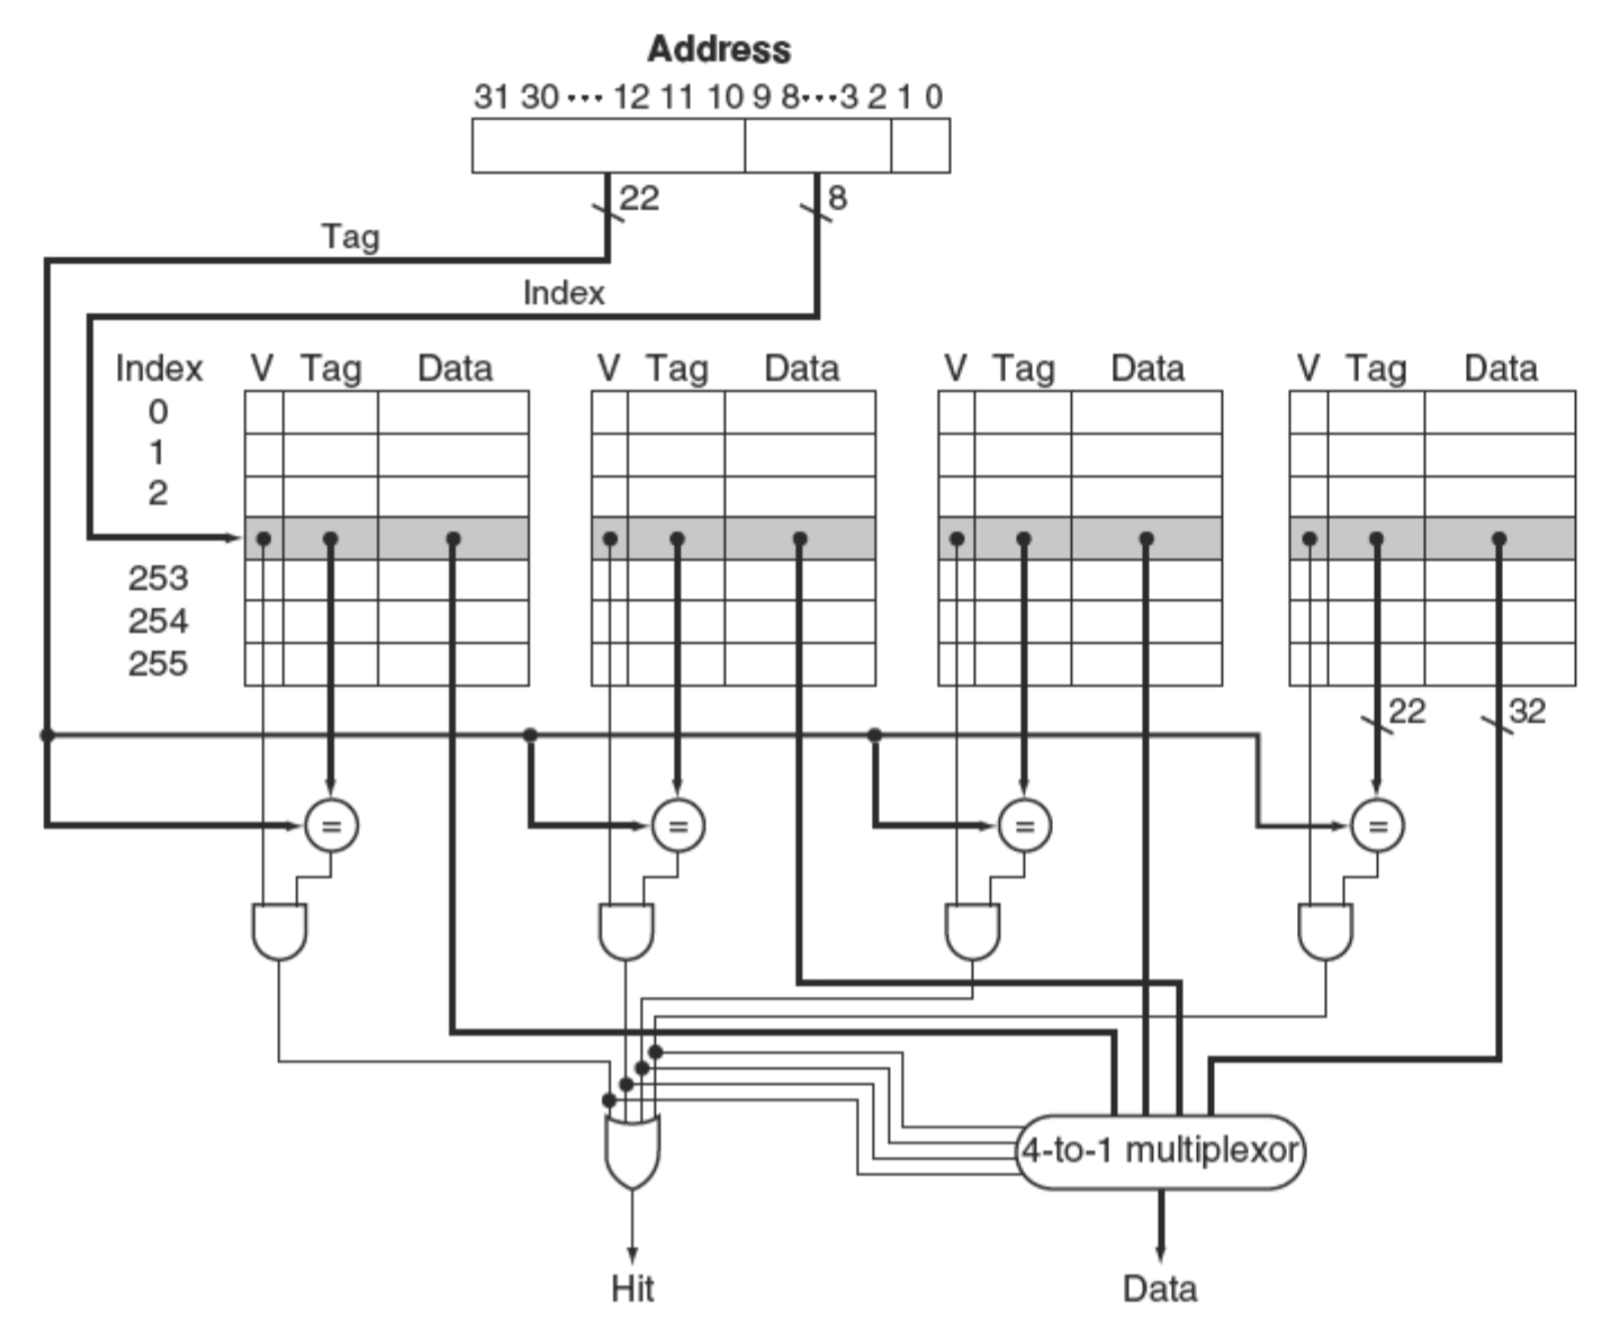
\includegraphics[width=1.0\textwidth]{pictures/4setassociativecache.png}
    }
    \caption{Implementation of a four-way set-associative cache}
  \end{figure}

  The choice among direct-mapped, set-associative, or fully associative mapping in any memory hierarchy will depend on the cost of a miss vs. the cost of implementing associativity, both in time and in extra hardware.

  \subsection{Choosing Which Block to Replace}
  When a miss occurs in a direct-mapped cache, the requested block can go in exactly on position, and the block occupying that position must be replaced. \\
  In a set associative cache, there's the choice of where to place the requested block, and hence a choice of which block to replace. \\
  In a set-associative cache, we must choose among the blocks in the selected set. \\

  The most commonly used scheme is \emph{least recently used} (LRU).
  In an LRU scheme, the block replaced is the once that has been unused for the longest time. \\

  LRU replacement is implemented by keeping track of when each element in a set was used relative to the other elements in the set.
  For a two-way set-associative cache, tracking when the two elements were used can be implemented by keeping a single bit in each set and setting the bit to indicate an element whenever that element is referenced.
  As associativity increases, implementing LRU becomes harder.

  \subsection{Reducing the Miss Penalty Using Multilevel Caches}
  Most microprocessors support an additional level of caching to close the gap between fast clock rates of modern processors and the increasingly long time to access DRAMs.
  This second-level cache is normally on the same chip and is accessed whenever a miss occurs in the primary cache.
  If the second-level cache contains the desired data, the miss penalty for the first-level cache is much less than than the access time of main memory.
  If neither cache contains the data, a main memory access is required, and a larger miss penalty is incurred. \\

  A two-level cache structure allows the primary cache to focus on minimizing hit time to yield a shorter clock cycle or fewer pipeline stages, while allowing the secondary cache to focus on miss rate to reduce the penalty of long memory access times. \\

  The primary cache of a \emph{multilevel cache} is often smaller, it may also use a smaller block size, to go with the smaller cache size and also to reduce the miss penalty. \\
  In comparison, the secondary cache will be much larger than in a single-level cache, since the access time of the secondary cache is less critical.
  With a larger total size, the secondary cache may use a larger block size than appropriate with a single-level cache.
  It often uses higher associativity than the primary cache given the focus of reducing miss rates.

  \subsection{Software Optimization via Blocking}
  When dealing with arrays, we can get good performance from the memory system if we store the array in memory so that accesses to the array are sequential in memory. \\
  However if we're dealing with multiple arrays, with some arrays accessed by rows and some by columns.
  Storing the arrays row-by-row (\emph{row major order}) or column-by-column (\emph{column major order}) does not solve the problem because both rows and columns are used in every loop iteration. \\

  Instead of operating on entire rows or columns of an array, \emph{blocked} algorithm operate on sub-matrices or \emph{blocks}.
  The goal is maximize accesses to the data loaded into the cache before the data are replaced;
  that is, improve temporal locality to reduce cache misses.

  \section{Dependable Memory Hierarchy}
  \subsection{Defining Failure}
  Suppose we have a specification of proper service.
  Which we can then see a system alternating between two states of delivered service with respect to the service specification:
  \begin{enumerate}
    \item \emph{Service accomplishment}, where the service is delivered as specified
    \item \emph{Service interruption}, where the delivered services is different from the specified services
  \end{enumerate}
  Transitions from state 1 to state 2 are caused by \emph{failures}, and transitions from state 2 to state 1 are called \emph{restorations}.
  Failures can be permanent or intermittent;
  it is more difficult to diagnose the problem when a system oscillates between the two states (intermittent failures).
  Permanent failures are much easier to diagnose. \\

  This definitions leads to two related terms: \emph{reliability} and \emph{availability}. \\

  \emph{Reliability} is a measure of the continuous service accomplishment---or, equivalently, of the time of failure---from a reference point.\\
  \emph{Mean time to failure} (MTTF) is a reliability measure. \\
  A related term is \emph{annual failure rate} (AFR), which is just the percentage of devices that would be expected to fail in a year for a given MTTF.
  When MTTF gets large it can be misleading, while AFR leads to better intuition. \\
  Service interruption is measure as \emph{mean time to repair} (MTTR). \\
  \emph{Mean time between failures} (MTBF) is simply the sum of MTTF + MTTR.
  Although MTBF is widely used, MTTF is often the more appropriate term. \\

  \emph{Availability} is then a measure of service accomplishment with respect to the alternation between the two states of accomplishment and interruption.
  It is statistically defined as:
  $$\text{Availability} = \frac{\text{MTTF}}{\text{MTTF} + \text{MTTR}} = \frac{\text{MTTF}}{\text{MTBF}}$$

  Both reliability and availability are quantifiable measures, rather than just synonyms for dependability. \\
  Shrinking MTTR can help availability as much as increasing MTTF. \\

  To increase MMTF, you can improve the quality of the components or design systems to continue operation in the presence of components that have failed.
  Hence, failure needs to be defined with respect to a context, as failure of a component may not lead to a failure of the system. \\
  The term \emph{fault} is used to mean failure of a component. \\
  Three ways to improve MTTF (mean time to failure):
  \begin{enumerate}
    \item \emph{Fault avoidance}: Preventing fault occurrence by construction
    \item \emph{Fault tolerance}: Using redundancy to allow the service to comply with the service specification despite faults occurring
    \item \emph{Fault forecasting}: \textbf{Predicting} the presence and creating of faults, allowing the component to be replaced before it fails
  \end{enumerate}

  \subsection{The Hamming Single Error Correcting, Double Error Detecting Code (SEC/DED)}
  Richard Hamming invented a popular redundancy scheme for memory. \\
  To invent redundant codes, we need to find how ``close'' correct bit patterns can be.
  The \emph{Hamming distance} is the minimum number of bits that are different between any two correct bit patterns.
  For example, the distance between 011011 and 001111 is two. \\
  Suppose the minimum distance between members of a code is two, and there's a one-bit error.
  It will turn a valid pattern in a code to an invalid one. \\
  If we can detect whether members of a code are valid or not,  we can detect single bit errors, and say we have single bit \emph{error detection code}. \\

  Hamming used a \emph{parity code} for error detection.
  In a parity code, the number of 1s in a word is counted;
  the word has odd parity if the number of 1s is odd and even otherwise.
  When a word is written into memory, the parity bit is also written (1 for odd, 0 for even).
  The parity of the $(n + 1)$ bit word should always be even;
  if a word of odd parity, then appending 1 after the rightmost bit result in even number of 1s, whereas a word of even parity would have 0 appended and retain its even parity.
  Then, when the word is read out, the parity bit is read and checked.
  If the parity of the memory word and the stored parity bit do not match, an error has occurred.
  \newline
  If there are 2 bits of error, then a 1-bit parity scheme will not detect any errors, since the parity will match the data with two errors. \\

  A parity code cannot correct errors but Hamming wanted to detect and correct errors.
  If a code with a minimum distance of 3 is used, then any single bit error would be closer to the correct pattern than to any other valid pattern.
  Hamming came up with a mapping of data into a distance 3 code called \emph{Hamming Error Correction Code} (ECC).
  We use extra parity bits to allow the position identification of a single error.
  Steps to calculate Hamming ECC:
  \begin{enumerate}
    \item Start numbering bits from 1 on the left, as opposed to numbering the rightmost bit as 0
    \item Mark all bit positions that are powers of 2 as parity bits (positions 1, 2, 4, 8, \dots)
    \item All other bit positions are used for data bits (positions 3, 5, 6, 7, 9, \dots)
    \item The position of parity bit determines sequence of data bits that it checks is:
    \begin{itemize}
      \item Bit 1 (0001\textsubscript{two}) check bits (1, 3, 5, 7, 9, 11, \dots), which are bits where rightmost bit of address is 1
      (0001\textsubscript{two}, 0011\textsubscript{two}, 0101\textsubscript{two},
      0111\textsubscript{two}, 1001\textsubscript{two}, 1011\textsubscript{two}, \dots)
      \item Bit 2 (0010\textsubscript{two}) checks bits (2, 3, 6, 7, 10, 11, 14, 15, \dots), which are bits where the second bit to the right in the address is 1
      \item Bit 4 (0100\textsubscript{two}) check bits (4-7, 12-15, 20-23, \dots), which are the bits where the third bit to the right in the address is 1
      \item Bit 8 (1000\textsubscript{two}) check bits (8-15, 24-31, 40-47, \dots), which are the bits where the fourth bit to the right in the address is 1
    \end{itemize}
    Note that each data bit is covered by two or more parity bits
    \item Set parity bits to create even parity for each group
  \end{enumerate}

  \begin{ex} Hamming ECC \\
  Using Hamming ECC for a one byte data value of 1001 1010\textsubscript{two}. \\
  Leaving spaces for the parity bits, the 12 bits pattern is \_ \_ 1 \_ 0 0 1 \_ 1 0 1 0 \\
  Position 1 checks for: \textcolor{red}{\_} \_ \textcolor{red}{1} \_ \textcolor{red}{0} 0 \textcolor{red}{1} \_ \textcolor{red}{1} 0 \textcolor{red}{1} 0; so parity bit 1 is set to 0 \\
  Position 2 checks for: 0 \textcolor{red}{\_} \textcolor{red}{1} \_ 0 \textcolor{red}{0} \textcolor{red}{1} \_ 1 \textcolor{red}{0} \textcolor{red}{1} 0;  so parity bit 2 is set to 1 \\
  Position 4 checks for: 0 1 1 \textcolor{red}{\_} \textcolor{red}{0} \textcolor{red}{0} \textcolor{red}{1} \_ 1 0 1 \textcolor{red}{0}; so parity bit 4 is set to 1 \\
  Position 8 checks for: 0 1 1 1 0 0 1 \textcolor{red}{\_} \textcolor{red}{1} \textcolor{red}{0} \textcolor{red}{1} \textcolor{red}{0}; so parity bit 8 is set to 0 \\

  The final word is 0111 0010 1010\textsubscript{two} \\
  Suppose we invert bit 10, then the word is 0111 0010 1\textcolor{red}{1}10\textsubscript{two} \\
  Parity bit 1 is 0 (four 1s, so even parity; this group is okay) \\
  Parity bit 2 is 1 (five 1s, so odd parity; there is an error somewhere) \\
  Parity bit 4 is 1 (two 1s, so even parity; this group is okay) \\
  Parity bit 8 is 1 (three 1s, so odd parity; there is an error somewhere) \\
  Since parity bits 2 and 8 are both wrong, $2 + 8 = 10$ so bit 10 is wrong. \\
  By inverting bit 10, we get 0111 0010 1\textcolor{red}{0}10\textsubscript{two}, done!
  \end{ex}

  At the cost of one more bit, the minimum Hamming distance in a code can be 4.
  Which means we can correct single bit \emph{errors} and \emph{detect double bit errors}. \\
  The idea is to add a parity bit that is calculated over the whole word.
  For example of a four-bit data word, which would only require 7 bits for single bit error detection.
  Hamming parity bits H (p\textsubscript{1}, p\textsubscript{2}, p\textsubscript{3}) are computed (even parity as usual) plus the even parity over the entire word, p\textsubscript{4}. \\
  Then the algorithm to correct one error and detect two is just to calculate parity over the ECC groups (H) as before plus one more over the whole group (p\textsubscript{4}).
  There are four cases:
  \begin{enumerate}
    \item H is even and p\textsubscript{4} is even, so no error occurred
    \item H is odd and p\textsubscript{4} is odd, so a correctable single single error occurred. (p\textsubscript{4} should calculate odd parity if one error occurred)
    \item H is even and p\textsubscript{4} is odd, a single error occurred in p\textsubscript{4} bit, not in the rest of the word, so correct the p\textsubscript{4} bit
    \item H is odd and p\textsubscript{4} is even, a double error occurred. (p\textsubscript{4} should calculate even parity if two errors occurred)
  \end{enumerate}
  Single Error Correcting / Double Error Detecting (SEC/DED) is common in memory for servers. \\
  Conveniently, eight byte data blocks can get SEC/DED with just one more byte, which is why many DIMMs are 72 bits wide.

  \newpage
  \section{Virtual Machines}
  \emph{Virtual Machines} (VMs) have gained popularity due to:
  \begin{itemize}
    \item The increasing importance of isolation and security in modern systems
    \item The failures in security and reliability of standard operating systems
    \item The sharing of a single computer among many unrelated users, in particular for cloud computing
    \item The dramatic increases in raw speed of processors over the decades, which makes the overhead of VMs more acceptable
  \end{itemize}
  The broadest definition of VMs includes all emulation methods that provide a standard software interface. \\
  We are interested in VMs that provide a complete system-level environment at the binary \emph{instruction set architecture} (ISA) level.
  Although some VMs run different ISAs in the VM from the native hardware, we assume they always match the hardware;
  such VMs are called (Operating) \emph{System Virtual Machines}. \\

  System virtual machines present the illusion that the users have an entire computer to themselves, including a copy of the OS.
  A single computer runs multiple VMs and can support a number of different OSes.
  On a conventional platform, a single OS ``owns'' all the hardware resources, but with a VM, multiple OSes all share the hardware resources. \\

  The software that supports VMs is called a \emph{virtual machine monitor} (VMM) or \emph{hypervisor};
  the VMM is the heart of VM technology. \\
  The underlying platform is called the \emph{host}, and its resources are shared among the \emph{guest} VMs/
  The VMM determines how to map virtual resources to physical resources: a physical resource may be time-shared, partitioned, or even emulated in software. \\

  In additional for using VMs for improving protection, VMs also provide two other significant benefits:
  \begin{enumerate}
    \item \emph{Managing software}. VMs provide an abstraction that can run the complete software stack, even including old operating systems like DOS.
    A typical deployment might be some VMs running legacy OSes, many running the current stable OS release, and a few testing the next OS release.
    \item \emph{Managing hardware}. One reason for multiple servers is to have each application running with the compatible version of the operating system on separate computers, as this separation can improve dependability.
    VMs allow these separate software stacks to run independently yet share hardware, thereby consolidating the number of servers.
  \end{enumerate}

  The cost of processor virtualization depends on the workload.
  User-level processor-bound programs have zero virtualization overhead, because the OS is rarely invoked, so everything runs at native speeds. \\
  Input/Output-intensive workloads are also OS-intensive, executing many system calls and privileged instructions that can result in high virtualization overhead.
  On the other hand, if the I/O-intensive workload is also \emph{I/O-bound}, the cost of processor virtualization can be completely hidden, since the processor is often idle waiting for I/O. \\

  The overhead is determined by both the number of instructions that must be emulated by the VMM and by how much time each takes to emulate them.

  \subsection{Requirements of a Virtual Machine Monitor}
  A VM Monitor presents a software interface to guest software, it must isolate the state of guests from each other, and it must protect itself from guest software (including guest OSes). \\
  The qualitative requirements for VMM are:
  \begin{itemize}
    \item Guest software should behave on a VM exactly as if it were running on the native hardware, except for performance-related behavior or limitations of fixed resources shared by multiple VMs.
    \item Guest software should not be able to change allocation of real system resources directly.
  \end{itemize}
  The VMM must control many tasks---access to privileged state, I/O, exceptions, and interrupts---even though the guest VM and OS currently running are temporarily using them. \\

  To be in charge, the VMM must be at a higher privilege level than the guest VM, which generally runs in user mode;
  this also ensures that the execution of any privileged instruction will be handled by the VMM.
  The basic requirements of system virtual:
  \begin{itemize}
    \item At least two processor modes, system and user.
    \item A privileged subset of instructions that is available only in system mode, resulting in a trap if executed in user mode;
    all system resources must be controllable only via these instructions.
  \end{itemize}

  \subsection{(Lack of) Instruction Set Architecture Support for Virtual Machines}
  If VMs are planned for during the design of the ISa, it is relatively easy to reduce both the number of instructions that must be executed by a VMM and improve their emulation speed. \\
  An architecture that allows the VM to execute directly on the hardware earns the title \emph{virtualizable} (the IBM 370 architecture has this label). \\

  Many instructions sets, such as x86, ARMv7, and MIPS, were created without virtualization. \\

  The VMM must ensure that the guest system only interacts with virtual resources, so a conventional guest OS runs as a user mode program on top of the VMM. \\
  If a guest OS attempts to access or modify information related to hardware resources via a privileged instruction, it will trap to the VMM.
  The VMM can then effect the appropriate changes to corresponding real resources. \\

  In the absence of such support, other measures must be taken.
  A VMM must take special precautions to locate all problematic instructions and ensure that they behave correctly when executed by a guest OS, thereby increasing the complexity of the VMM and reducing the performance of running the VM.

  \subsection{Protection and Instruction Set Architecture}
  Protection is a joint effort of architecture and OSes, but architects had to modify some awkward details of existing instruction set architectures when virtual memory became popular. \\

  VMM took three steps to improve performance of virtual machines:
  \begin{enumerate}
    \item Reduce the cost of processor virtualization
    \item Reduce interrupt overhead cost due to virtualization
    \item Reduce interrupt cost by steering interrupts to the proper VM without invoking the VMM
  \end{enumerate}

  \section{Virtual Memory}
  Caches provide fast access to recently used portions of a program's code and data.
  Similarly, the main memory can act as a ``cache'' for the secondary storage, usually implemented with magnetic disks.
  This is called \emph{virtual memory}. \\

  Historically, the major motivations for virtual memory are:
  \begin{enumerate}
    \item To allow efficient and safe sharing of memory among multiple programs, such as for the memory needed by multiple virtual machines for cloud computing.
    \item To remove the programming burdens of a small, limited amounted of main memory.
  \end{enumerate}
  Now, the first reason still stands for virtual memory. \\

  To allow multiple virtual machines to share the same memory, we must be able to protect the virtual machines from each other, ensuring that a program can only read and write the portions of main memory that have been assigned to it.
  Main memory only needs to contain the active portions of the many virtual machines,just as a cache contains only the active portion of one program. \\
  The principle of locality enables virtual memory as well as caches, and virtual memory allows us to efficiently share the processor as well as the main memory. \\

  The VMs sharing the memory change dynamically while the VMs are running.
  Due to this dynamic interaction, each program need to be compiled into its own \emph{address space}---a separate range of memory locations accessible only to this program.
  Virtual memory implements the translation of a program's address space to \emph{physical addresses}.
  This translation process enforces \emph{protection} of a program's address space from other virtual machines. \\

  The second motivation for virtual memory is to allow a single user program to exceed the size of primary memory.
  Virtual memory automatically manages the two levels of the memory hierarchy represented by main memory (sometimes called \emph{physical memory} to distinguish it from virtual memory) and secondary storage. \\

  A virtual memory block is called a \emph{page}, and a virtual memory miss is called a \emph{page fault}.
  With virtual memory, the processor produces a \emph{virtual address}, which is translated by a combination of hardware and software to a \emph{physical address}, which is used to access main memory.

  \begin{figure}[!htp]
  \centering{
    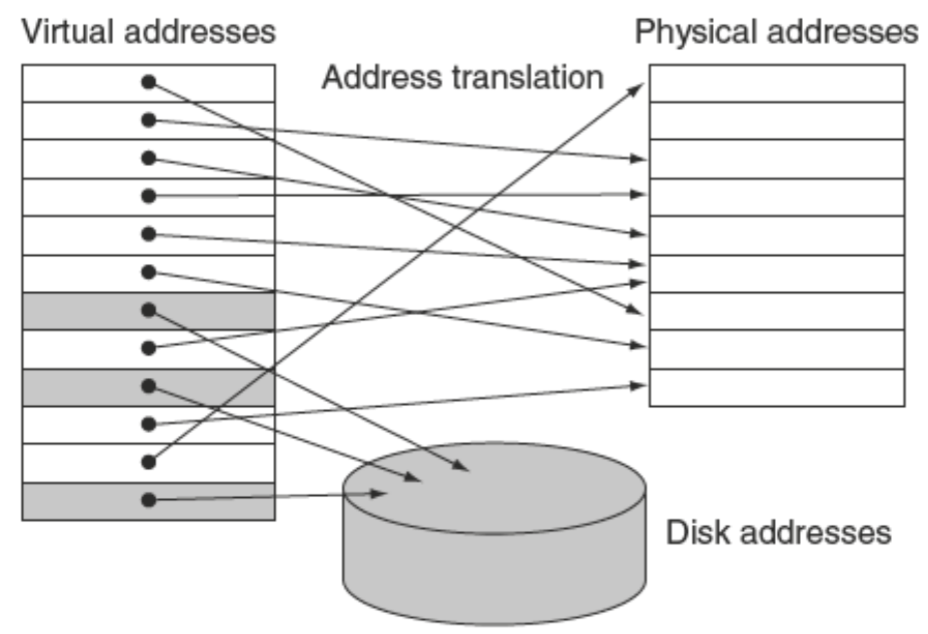
\includegraphics[width=0.6\textwidth]{pictures/addressMapping.png}
  }
  \end{figure}

  The figure above shows the virtually addressed memory with pages mapped to main memory.
  The process is \emph{address mapping} or \emph{address translation}. \\

  The two memory hierarchy levels controlled by virtual memory are usually DRAMs and flash memory in personal mobile devices and DRAMs and magnetic disks in servers. \\

  Virtual memory simplifies loading the program for execution by providing \emph{relocation}.
  Relocation maps the virtual addresses used by a program to different physical addresses before the addresses are used to access memory.
  This relocation allows a program to be loaded anywhere in main memory.
  All virtual memory systems in use today relocate the program as a set of fixed-size blocks (pages), thereby eliminating the need to find a contiguous block of memory to allocate to a program;
  instead, the OS only need to find a sufficient number of pages in main memory. \\

  In virtual memory, the address is broken into a \emph{virtual page number} and a \emph{page offset}.

  \begin{figure}[H]
  \centering{
    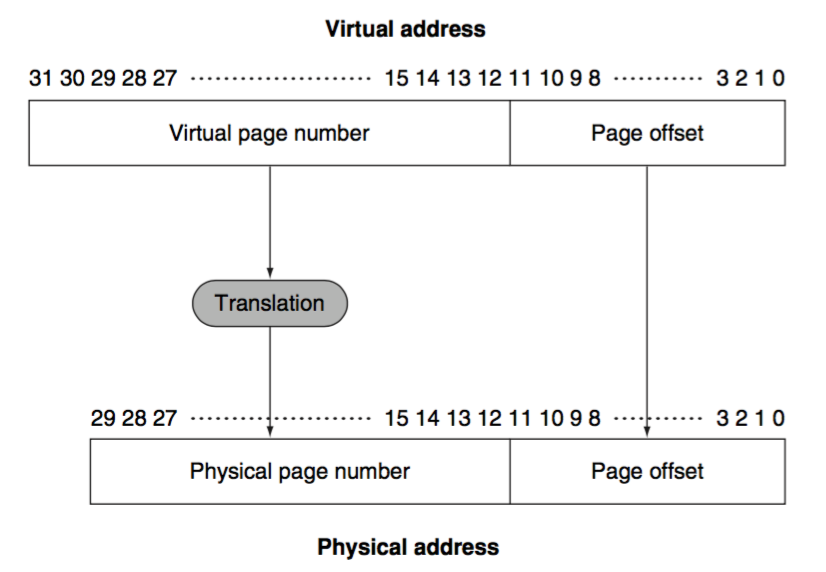
\includegraphics[width=0.6\textwidth]{pictures/vAddressMapToPAddress.png}
    \caption{Mapping from a virtual to a physical address}
  }
  \end{figure}

  The figure above shows how a virtual address space of 4 GiB maps to the main memory space of 1 GiB (physical page number is 18, so $2^{18}$ allows 1 GiB). \\
  The physical page number constitutes the upper portion of the physical address, while the page offset, which is not changed, constitutes the lower portion.
  The number of bits in the page offset field determines the page size.
  The number of pages addressable with the virtual address need not match the number of pages addressable with the physical address. \\
  Having a larger number of virtual pages than physical pages is the basis for the illusion of an essentially unbounded amount of virtual memory. \\

  The high cost of a page fault motivates many design choices in virtual memory systems.
  A \emph{page fault} to disk will take millions of clock cycles to process.
  This miss penalty, dominated by the time to get the first word for typical page sizes, leads to several key decisions in designing virtual memory systems:
  \begin{itemize}
    \item Pages should be large enough to try to amortize the high access time.
    Sizes from 4 KiB to 16 KiB are typical today.
    New desktops and server systems are being developed to support 32 KiB and 64 KiB pages, but new embedded systems are going to 1 KiB pages
    \item Organizations that reduce the page fault rate are preferred.
    The primary technology used here is to allow fully associative placement of pages in memory
    \item Page faults can be handled in software because the overhead will be small compared to the disk access time.
    In addition, software can afford to use clever algorithms for choosing how to place pages because even small reductions in the miss rate will pay for the cost of such algorithms
    \item Write-through will not work for virtual memory, since writes takes too long.
    Instead, virtual memory systems use write-back.
  \end{itemize}

  \subsection{Placing a Page and Finding It Again}
  Due to the high penalty for a page fault, designers reduce page fault frequency by optimizing page placement.
  If a virtual page is allowed to be mapped to any physical page, the operating system can then choose to replace any page it wants when a page fault occurs. \\
  The ability to use a clever and flexible replacement scheme reduces the page fault rate and simplifies the use of fully associative placement of pages. \\

  The difficulty of using fully associative is in locating an entry, since it can be anywhere in the upper level of the hierarchy.
  A full search is impractical. \\
  In virtual memory systems, we locate pages by using a table that indexes the memory called a \emph{page table}, which resides in memory.
  A page table is indexed with the page number from the virtual address to discover the corresponding physical page number.
  Each program has its own page table, which maps the virtual address space of that program to main memory. \\
  To indicate the location of the page table in memory, the hardware includes a register that points to the start of the page table;
  this is called the \emph{page table register}. \\

  The page table, together with the program counter and the registers, specifies the \emph{state} of a virtual machine.
  If another virtual machine is allowed to use the processor, we must save this state.
  Later, after restoring this state, the virtual machine can continue execution.
  This state is often referred to as a \emph{process}. \\
  The process is considered \emph{active} when it is in possession of the processor;
  \emph{inactive} otherwise. \\

  The figure below uses a page table register, the virtual address, and the indicated page table to show how the hardware can form a physical address.

  \begin{figure}[H]
  \centering{
    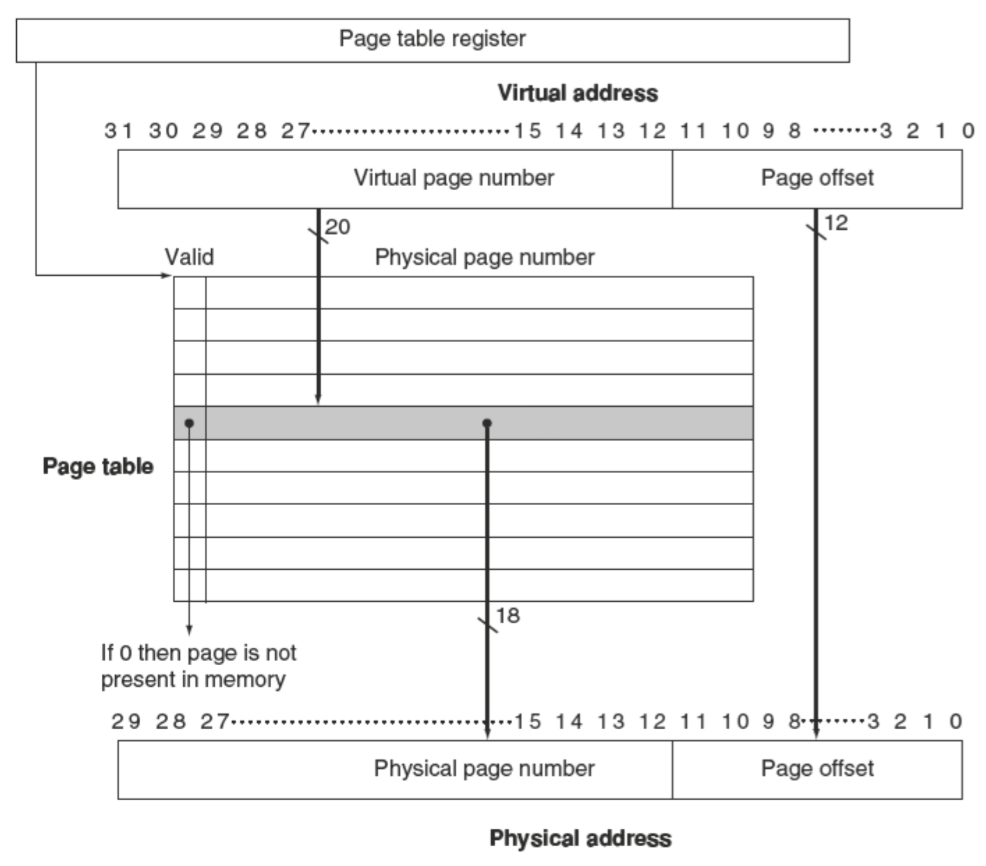
\includegraphics[width=0.75\textwidth]{pictures/pageTable.png}
  }
  \end{figure}

  A valid bit is used in each page table entry.
  If the bit if off, the page is not present in main memory and a page fault occurs.
  If the bit is on, the page is in memory and the entry contains the physical page number.
  The page table contains a mapping for every possible virtual page, so no tags are required. \\
  The index that is used to access the page table consists of the full block address, which is the virtual page number.

  \subsection{Page Faults}
  If the valid bit for a virtual page is off, a page fault occurs.
  The OS must be given control, which is done with the exception mechanism.
  Once it gets control, it must find the page in the next level of the hierarchy (usually flash memory or magnetic disk) and decide where to place the requested page in main memory. \\

  The virtual address alone does not immediately tell us where the page is on the disk.
  We must keep track of the location on disk of each page in virtual address space. \\

  Since a page in memory cannot be known in advance if it is to be replaced, the OS usually creates the space on flash memory or disk for all the pages of a process when it creates the process.
  This space is called the \emph{swap space}.
  The OS also creates a data structure to record where each virtual page is stored on disk.
  The data structure may be part of the page table or may be an auxiliary data structure indexed in the same way as the page table.

  \begin{figure}[H]
  \centering{
    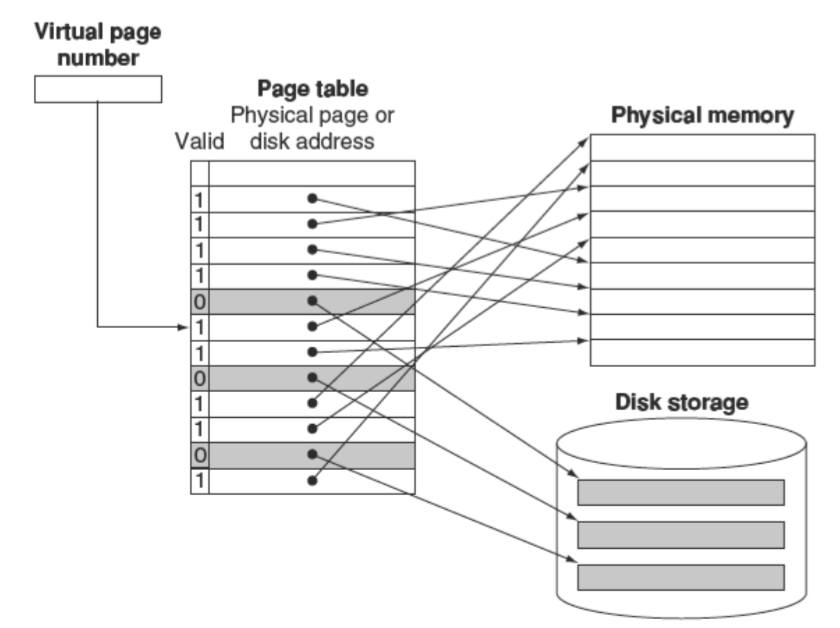
\includegraphics[width=0.7\textwidth]{pictures/pageTableMappings.png}
  }
  \end{figure}

  In the figure above, the page table maps each page in virtual memory to either a page in main memory or a page stored on disk, which is the next level in the hierarchy. \\

  The OS also creates a data structure that tracks which processes and which virtual addresses use each physical page.
  When a page fault occurs, if all the pages in main memory are in use, the operating system must choose a page to replace.
  Since we want to minimize the number of page faults, most OSes try to choose a page that is hypothesized to be not needed in the near future;
  OSes use the \emph{least recently used} (LRU) replacement scheme to use the past to predict the future.
  The replaced pages are written to swap space on the disk. \\

  \textbf{Elaboration}: \\
  A range of techniques is used to reduce the amount of storage required for the page table.
  The following five techniques aim at reducing the total maximum storage required as well as minimizing the main memory dedicated to page tables:
  \begin{enumerate}
    \item Keep a limit register that restricts the size of the page table for a given process.
    Requires that the address space expand in only one direction
    \item Most languages require two areas whose size is expandable: one area holds the stack and the other area holds the heap.
    Due to this duality, it is convenient to divide the page table and let it grow from the highest address down, as well as from the lowest address up.
    There will be two separate page tables and two separate limits.
    The major disadvantage of this scheme is that it does not work well when the address space is used in a sparse fashion rather than as a contiguous set of virtual addresses
    \item Apply a hash function to the virtual address so that the page table need only be only the size of the number of physical pages in main memory.
    This structure is called an \emph{inverted page table}
    \item Multiple levels of page tables can reduce the total amount of page table storage.
    This is useful with very large address spaces and in software systems that require noncontiguous allocation.
    The primary disadvantage is the more complex process for address translation
    \item Allow the page tables to be paged.
  \end{enumerate}
  For more details, refer to page 436 (Section 5.7) in ``Computer Organization and Design''

  \subsection{What about Writes?}
  The different between access time to the cache and main memory is tens to hundreds of cycles, and write-through schemes can be used, although we need a write buffer to hide the latency of the write from the processor. \\
  In a virtual memory system, writes to the next level of the hierarchy (disk) can take millions of processor clock cycles;
  therefore, building a write buffer to allow the system to write-through to disk would be impractical.
  Instead, virtual memory systems must use write-back, performing the individual writes into the page in memory, and copying the page back to disk when it is replaced in memory. \\

  Disk transfer time is small compared with its access time, copying back an entire page is much more efficient than writing individual words back to the disk;
  thus, this is why write-back scheme has another advantage in a virtual memory system. \\
  A write-back operation is still costly, despite being more efficient than transferring individual words.
  We would like to know whether a page needs to be copied back when we choose to replace it.
  To track if a page has been written since it was read into the memory, a \emph{dirty bit} is added to the page table.
  The dirty bit is set when any word in a page is written. \\
  If the OS replaces the page, the dirty bit indicates if the page needs to be written out before its location in memory can be given to another page. \\
  A modified page is often referred as a \emph{dirty page}.

  \subsection{Making Address Translation Fast: the TLB}
  Since page tables are stored in main memory, every memory access by a program can take at least twice as long: one memory access to obtain the physical address and a second access to get the data.
  To improve access performance, relying on locality of reference to the page table is key.
  When a translation for a virtual page number is used, it is likely to be needed again in the near future, because the references to the words on that page have both temporal and spatial locality. \\

  A special cache is included to keep track of recently used translations;
  it is referred to as a \emph{translation-lookaside buffer} (TLB), or it is more accurate to refer to it as a translation cache.

  \begin{figure}[H]
  \centering{
    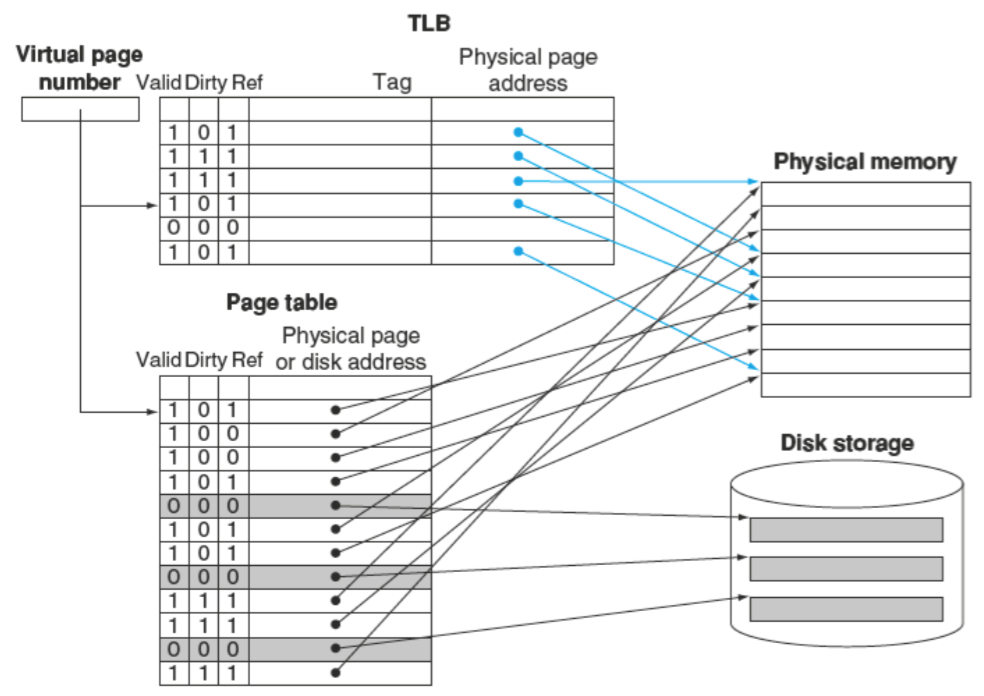
\includegraphics[width=0.7\textwidth]{pictures/TLB.png}
  }
  \end{figure}

  Each tag entry in the TLB holds a portion of the virtual page number, and each data entry of the TLB holds a physical page number.
  The TLB is accessed instead of the page table on every reference, so the TLB need to include other status bits, such as the dirty and the reference bits. \\
  The translations-lookaside buffer is a cache, so it must have a tag field.
  If there is no matching entry in the TLB for a page, the page table must be examined. \\
  The page table either supplies a physical page number for the page (which can then be used to build a TLB entry) or indicates that the page resides on disk, in which case a page fault occurs. \\
  Since the page table has an entry for every virtual page, no tag field is needed;
  unlike a TLB, a page table is \emph{not} a cache. \\

  On every reference, the virtual page number is looked up in the TLB. \\
  If there is a hit, the physical page number is used to form the address, and the corresponding reference bit is turned on. \\
  If the processor is performing a write, the dirty bit is also turned on. \\

  If a miss in the TLB occurs, we must determine if it is page fault or a TLB miss.
  If the page exists in memory, then the TLB miss indicates that the translation is missing.
  In such cases, the processor can handle the TLB miss by loading the translation from the page table into the TLB and then trying the reference again. \\
  If the page is not present in memory, then the miss indicates a page fault.
  In this case, the processor invokes the OS using an exception. \\
  The TLB has many fewer entries than the number of pages in main memory, TLB misses will be much more frequent than true page faults. \\

  TLB misses can be handled either in hardware or in software.
  There can be little performance differences between the two approaches, since the basic operations are the same for either case. \\

  After a TLB miss occurs and the missing translation has been retrieved from the page table, a TLB entry needs to be selected to be replaced.
  The reference and dirty bits are contained in the TLB entry, so these bits need to be copied back to the page table entry when an entry is replaced.
  These bits are the only portion of the TLB entry that can be changed. \\
  Using write-back---that is, copying these entries back at miss time rather than when they are written---is very efficient, since the TLB miss rate is expected to be small. \\

  Some typical values for a TLB might be:
  \begin{itemize}
    \item TLB size: 16-512 entries
    \item Block size: 1-2 page table entries (typically 4-8 bytes each)
    \item Hit time: 0.5-1 clock cycle
    \item Miss penalty: 10-100 clock cycles
    \item Miss rate: 0.01\%-1\%
  \end{itemize}

  Some systems use small, fully associative TLBs because a fully associative mapping has a lower miss rate;
  furthermore, the TLB is small, so the cost of a fully associative mapping is not too high. \\
  Other systems use large TLBs, often with small associativity. \\
  With a fully associative mapping, choosing the entry to replace becomes tricky since implementing a hardware LRU scheme is too expensive.
  In addition, TLB misses are much more frequent that page faults and thus must be handled more cheaply, so we cannot afford an expensive software algorithm (as we can for page faults). \\
  As a result, many systems provide some support for randomly choosing an entry to replace.

  \subsection{Integrating Virtual Memory, TLBs, and Caches}
  Virtual memory and cache systems work together as a hierarchy, so data cannot be in the cache unless it is present in main memory. \\
  The hierarchy is maintained with the help of the operating system which flushes the contents of any page from the cache when it decides to migrate the page to disk.
  At the same time, the OS modifies the page tables and TLB, so that an attempt to access any data on the migrated page will generate a page fault. \\

  In the best case, a virtual address is translated by the TLB and sent to the cache where the appropriate data is found, retrieved, and sent back to the processor. \\

  In the worst case, a reference can be miss in all three components of the memory hierarchy: the TLB, the page table, and the cache. \\

  Possible combinations of events in the TLB, virtual memory system, and cache in table below.
  \begin{center}
  \begin{tabular}{| c | C{1cm} | c | C{8cm} |}
  \hline
  TLB & Page Table & Cache & Possible? If so, under what circumstances? \\
  \hline
  Hit & Hit & Miss & Possible, although the page table is never really checked if TLB hits. \\
  \hline
  Miss & Hit & Hit & TLB misses, but entry found in page table; after retry, data is found in cache. \\
  \hline
  Miss & Hit & Miss & TLB misses, but entry found in page table; after retry, data misses in cache. \\
  \hline
  Miss & Miss & Miss & TLB misses and is followed by a page fault; after retry, data must miss in cache. \\
  \hline
  Hit & Miss & Miss & Impossible; cannot have a translation in TLB if page is not present in memory. \\
  \hline
  Hit & Miss & Hit & Impossible; cannot have a translation in TLB if page is not present in memory. \\
  \hline
  Miss & Miss & Hit & Impossible; data cannot be allowed in cache if the page is not in memory. \\
  \hline
  \end{tabular}
  \end{center}

  The table above assumes that all memory addresses are translated to physical addresses before the cache is accessed. \\
  The cache is \emph{physically indexed} and \emph{physically tagged} (both the cache index and tag are physical, rather than virtual addresses). \\
  The amount of time to access memory, assuming a cache hit, must accommodate both a TLB access and a cache access;
  these accesses can be \emph{pipelined}. \\

  Alternatively, The processor can index the cache with an address that is completely or partially virtual.
  This is called a \emph{virtually addressed cache}, and it uses tags that are virtual addresses;
  hence, such a ache is \emph{virtually indexed} and \emph{virtually tagged}. \\
  In such caches, the address translation hardware (TLB) is unused during normal cache access, since the cache is accessed with a virtual address that has not been translated to a physical address. \\
  This takes the TLB out of the critical path, reducing cache latency.
  However, when a cache miss occurs, the processor needs to translate the address to a physical address so that it can fetch the cache block from main memory. \\

  When the cache is accessed with a virtual address and pages are shared between processes, there is a possibility of \emph{aliasing}.
  Aliasing is a situation in which two addresses access the same object;
  it can occur in virtual memory when there are two virtual address for the same physical page. \\
  The ambiguity creates an issue, because a word on such a page may be cached in two different locations, each corresponding to different virtual addresses.
  The ambiguity allows one program to write the data without the other program being aware that the data had changed. \\
  Completely virtually addressed caches either introduce design limitations on the cache and TLB to reduce aliases or require the OS, and perhaps the user as well, to take steps to prevent aliases. \\

  A compromise between the two design points is caches that are virtually indexes---sometimes using just the page-offset portion of the address, which is really a physical address since it is not translated---but use physical tags.
  These designs, which are \emph{virtually indexed} but \emph{physically tagged}, attempts to achieve the performance advantages of virtually indexed caches with the architecturally simpler advantage of a \emph{physically addressed cache}. \\
  However, there must be careful coordination between the minimum page size, the cache size, and associativity. \\

  \subsection{Implementing Protection with Virtual Memory}
  The most important function of virtual memory is to allow sharing of a single main memory by multiple processes, while providing memory protection among these processes and the operating system. \\
  The protection mechanism must ensure that although multiple processes are sharing the same main memory, one renegade process cannot write into the address space of another user process or into the OS either intentionally or unintentionally.
  The write access bit in the TLB can protect a page from being written.
  Without this level of protection, viruses would be even more widespread. \\

  To enable the OS to implement protection in the virtual memory system, the hardware must provide at least the three basic capabilities (note that the first two are the same requirements for VMs):
  \begin{enumerate}
    \item Support at least two modes that indicate whether the running process is a user process or an OS process, variously called a \emph{supervisor} process, a \emph{kernel} process, or an \emph{executive process}
    \item Provide a portion of the processor state that a user process can read but not write.
    This includes the user/supervisor mode bit, which dictates whether the processor is in user or supervisor mode, the page table pointer, and the TLB.
    The OS uses special supervisor mode only instruction to write these elements
    \item Provide mechanisms whereby the processor can go from user mode to supervisor mode and vice versa.
    The first direction is typically accomplished by a \emph{system call} exception, implemented as a special instruction (\emph{syscall} in MIPS) that transfers control to a dedicated location in supervisor code space.
    As with any other exception, the PC from the point of the system call is saved in the exception PC (EPC), and the processor is placed in supervisor mode.
    To return to user mode from the exception, use the \emph{return from exception} (ERET) instruction, which resets to user mode and jumps to the address in EPC
  \end{enumerate}

  By using these mechanisms and storing the page tables in the operating system's address space, the OS can change the page table while preventing a user process from changing them, ensuring that a user process can access only the storage provided to it by the OS. \\

  Each process has its own virtual address space.
  If the OS keeps the page tables organized so that the independent virtual pages map to disjoint physical pages, one process will not be able to access another's data. \\
  This of course requires a user process be unable to change the page table mapping.
  Thus, the page tables can be placed in the protected address space of the operating system such that the OS can modify the page tables but not any user processes. \\

  When processes want to share information in a limited way, the OS must assist them, since accessing the information of another process requires changing the page table of the accessing process.
  The write access bit can be used to restrict the sharing to just reading, and this bit can only be changed by the operating system. \\
  Any bits that determine the access rights for a page must be included in both the page table and the TLB, because the page table is accessed only on a TLB \emph{miss}.

  \subsection{Handling TLB Misses and Page Faults}
  A TLB miss occurs when no entry in the TLB matches a virtual address. \\
  A TLB miss can indicate one of two possibilities:
  \begin{enumerate}
    \item The page is present in memory, and we need only create the missing TLB entry
    \item The page is not present in memory, and we need to transfer control to the operating system to deal with a page fault
  \end{enumerate}

  MIPS handles a TLB miss in software.
  It brings the page table entry from memory and then re-executes the instruction that caused the TLB miss.
  Upon re-executing, it will get a TLB hit.
  If the page table entry indicates the page is not in memory, this time it will get a page fault exception. \\

  Handling a TLB miss or page fault requires using the exception mechanism to interrupt the active process, transferring control to the OS, and later resuming exception of the interrupted process.
  A page fault will be recognized sometime during the clock cycle used to access memory.
  To restart the instruction after the page fault is handled, the program counter of the instruction that caused the page fault must be saved in the exception program counter (EPC). \\

  In addition, a TLB miss or page fault exception must be asserted by the end of the same clock cycle that the memory access occurs, so that the next clock cycle will begin exception processing rather than continue normal instruction execution.
  If the page fault was not recognized in this clock cycle, a load instruction could overwrite a register, and it can cause disasters when the instruction is restarted. \\
  By deasserting the write control line to the memory, the write into memory can be prevented from completing when there is a page fault. \\

  Between the time we being executing the exception handler in the operating system and the time that the operating system has saved all the state of the process, the operating system is particularly vulnerable.
  For example, another exception can occur when processing the first exception in the operating system, the control unit would overwrite the EPC, making it impossible to return to the instruction that caused the page fault. \\
  This can be avoided by providing the ability to \emph{disable} and \emph{enable exceptions}.
  When an exception first occurs, the processor sets a bit that disables all other exceptions;
  this could happen at the same time the processor sets the supervisor mode bit. \\
  The OS will then save just enough state to allow it to recover if another exception occurs---namely, the EPC and Cause registers.
  The OS can then re-enable exceptions. \\
  These steps make sure that exceptions will not cause the processor to lose any state and thereby be unable to restart execution of the interrupting instructions. \\

  ONce the OS knows the virtual address that caused the page fault, it must complete the following steps:
  \begin{enumerate}
    \item Look up the page table entry using the virtual address and find the location of the referenced page on disk
    \item Choose a physical page to replace, if the chosen page is dirty, it must be written out to disk before a new virtual page can be brought into this physical page
    \item Start a read to bring the referenced page from disk into the chosen physical page
  \end{enumerate}

  The last step will take millions of processor clock cycles (so will the second if the replaced page is dirty);
  accordingly, the OS will usually select another process to execute in the processor until the disk access completes.
  Since the OS saves the state of the process, it can freely give control of the processor to another process. \\

  When the read of the page from disk is complete, the OS can restore the state of the process that originally caused the page fault and execute the instruction that returns from the exception.
  This instruction will reset the processor from kernel to user mode, as well as restore the program counter.
  The user process and re-executes the instruction that faulted, accesses the requested page successfully, and continues execution. \\

  Page fault exceptions for data accesses are difficult to implement properly in a processor because of combination of three characteristics:
  \begin{enumerate}
    \item They occur in the middle of instructions, unlike instruction page faults
    \item The instruction cannot be completed before handling the exception
    \item After handling the exception, the instruction must be restarted as if nothing had occurred
  \end{enumerate}
  Making instructions \emph{restartable}, so that the exception can be handled and the instruction later continued.
  Each instruction writes only one data item which occurs at the end of the instruction cycle.
  So the instruction can be prevented from completing by not writing and restart the instruction at the beginning.

  \subsection{Summary of Virtual Memory}
  Virtual memory is the level of memory hierarchy that manages caching between the main memory and secondary memory.
  Virtual memory allows a single program to expand its address space beyond the limits of main memory.
  Virtual memory supports sharing of the main memory among multiple, simultaneously active processes, in a protected manner. \\

  Managing the hierarchy between main memory and disk is challenging due to the high cost of page faults.
  Several techniques are used to reduce the miss rate:
  \begin{enumerate}
    \item Pages are made large to take advantage of spatial locality and to reduce the miss rate
    \item Thee mapping between virtual addresses and physical addresses, which is implemented with a page table, is made fully associative so that a virtual page can be placed anywhere in main memory
    \item The OS uses techniques, such as LRU and a reference bit, to choose which pages to replace
  \end{enumerate}
  Writes to secondary memory are expensive, so virtual memory uses a write-back scheme and also tracks whether a page is unchanged (using a dirty bit) to avoid writing unchanged pages. \\

  The virtual memory mechanism provides address translation from a virtual address used by the program to the physical address space used for accessing memory.
  The address translation allows protected sharing of the main memory and provides several additional benefits, such as simplifying memory allocation.
  Ensuring that processes are protected from each other requires that only the operating system can change the address translations, which is implemented by preventing user programs from changing the page tables.
  Controlled sharing of pages among processes can be implemented with the help of the operating system and access bits in the page table that indicate whether the user program has read or write access to a page. \\

  If a processor had to access a page table resident in memory to translate every access, virtual memory would be too expensive, as caches would be pointless.
  Instead, a TLB acts as a cache for translations from the page table.
  Addresses are then translated from virtual to physical using the translations in the TLB. \\

  Caches, virtual memory, and TLBs all rely on a common set of principles and policies.
  The next section discusses this common framework. \\

  If a program routinely accesses more virtual memory than it has physical memory, it will run very slowly.
  Such a program would be continuously swapping pages between memory and disk, called \emph{thrashing}.

  \section{A Common Framework for Memory Hierarchy}
  Many of the aspects of memory hierarchies differ quantitatively, but many of the policies and features that determine how a hierarchy functions are similarly qualitatively (shown in table below).
  \begin{center}
  \begin{tabular}{| C{2.5cm} | C{2cm} | C{2.5cm} | C{2.58cm} | C{2.1cm} |}
  \hline
  Feature & Typical values for L1 caches & Typical values for L2 caches
  & Typical values for paged memory & Typical values for a TLB \\
  \hline
  \small Total size in blocks & 250 - 2,000 & 2,500 - 25,000 & 16,000 - 250,000 & 40 - 1024 \\
  \hline
  \small Total size in kilobytes & 16 - 64 & 125 - 2,500 & 1,000,000 - 1,000,000,000 & 0.25 - 16 \\
  \hline
  \small Block size in bytes & 16 - 64 & 64 - 128 & 4,000 - 64,000 & 4 - 32 \\
  \hline
  \small Miss penalty in clocks & 10 - 25 & 100 - 1,000 & 10,000,000 - 100,000,000 & 10 - 1,000 \\
  \hline
  \small Miss rates (global for L2) & 2\% - 5\% & 0.1\% - 2\% & 0.00001\% - 0.0001\% & 0.01\% - 2\% \\
  \hline
  \end{tabular}
  \end{center}

  \subsection{Question 1: Where Can a Block Be Placed?}
  Block placement in the upper level of the memory hierarchy can use a range of schemes, from direct-mapped to set associative to fully associative.
  Note that the entire range of schemes can be thought of as variations on a set-associative scheme where the number of sets and the number of blocks per set varies:
  \begin{center}
  \begin{tabular}{| c | c | c |}
  \hline
  Scheme Name & Number of Sets & Blocks per Set \\
  \hline
  {\small Direct mapped} & {\small Number of blocks in cache} & {\small 1} \\
  \hline
  {\small Set associative}
  & $\frac{\text{Number of blocks in the cache}}{\text{Associativity}}$
  & {\small Associativity (typically 2 - 16)} \\
  \hline
  {\small Fully associative} & {\small 1} & {\small Number of blocks in the cache} \\
  \hline
  \end{tabular}
  \end{center}
  The advantage of increasing the degree of associativity is that it usually decreases the miss rate.
  The improvement in miss rate comes from reducing misses that compete for the same location. \\
  As the cache size grow, the relative improvement from associativity increases only slightly;
  since the overall miss rate of a larger cache is lower, the opportunity for improving the miss rate decreases and the absolute improvement in the miss rate from associativity shrinks. \\
  The potential disadvantages of associativity are increases cost and slower access time.

  \subsection{Question 2: How Is a Block Found?}
  The block is located depending on the block placement scheme:
  \begin{center}
  \begin{tabular}{| c | c | c |}
  \hline
  Associativity & Location Method & Comparisons Required \\
  \hline
  {\small  Direct mapped} & {\small Index} & {\small 1} \\
  \hline
  {\small Set associative} & {\small Index the set, search among the elements}
  & {\small Degree of associativity} \\
  \hline
  {\small \multirow{2}{*}{Full}} & {\small Search all cache entries}
  & {\small Size of the cache} \\
  \cline{2-3}
  & {\small Separate lookup table} & {\small 0} \\
  \hline
  \end{tabular}
  \end{center}
  Including the L2 cache on the chip enables much higher associativity, because the hit times are not as critical and the designer does not have to rely on standard SRAM chips as the building blocks. \\
  Fully associative caches are prohibitive except for small sizes, where the cost of the comparators is not overwhelming and where the absolute miss rate improvements are greatest. \\

  In virtual memory systems, a separate mapping table---the page table---is kept to index the memory.
  In addition to the storage required for the table, using an index table requires an extra memory access.
  The choice of full associativity for page placement and the extra table is motivated by:
  \begin{enumerate}
    \item Full associativity is beneficial, since misses are very expensive
    \item Full associativity allows software to use sophisticated replacement schemes that are designed to reduce the miss rate
    \item The full map can be easily indexed with no extra hardware and no search required
  \end{enumerate}
  Therefore, virtual memory systems almost always use fully associative placement. \\

  Set-associative scheme is often used for caches and TLBs, where the access combines indexing and the search of a small set.

  \subsection{Question 3: Which Block Should Be Replaced on a Cache Miss?}
  When a miss occurs in an associative cache, a block must be replaced.
  In a fully associative cache, all blocks are candidates for replacement.
  If the cache is set associative, we must choose among the blocks in the set.
  Replacement is easy in a direct-mapped cache (only one candidate). \\

  Two primary strategies for replacement:
  \begin{enumerate}
    \item \emph{Random}: Candidates blocks are randomly selected, possibly using some hardware assistance
    \item \emph{Least recently used} (LRU): The block replaced is the one that has been unused for the longest time
  \end{enumerate}
  Practically, LRU is costly to implement for hierarchies with more than a small degree of associativity (typically two or four), since tracking the usage information is costly. \\

  For larger associativity, either LRU is approximated or random replacement is used. \\
  In caches, the replacement algorithm is in the hardware, so the scheme should be easy to implement.
  Random replacement is simply to build in hardware, and for a two-way set-associative cache, random replacement has a miss rate about 1.1 times higher than LRU replacement. \\
  As the caches become larger, the miss rate for both replacement strategies falls, and the absolute difference becomes small. \\
  Random replacement can sometimes be better than the simple LRU approximation that are easily implemented in hardware. \\

  In virtual memory, some form of LRU is always approximated, since even a tiny reduction in the miss rate can be important when the cost of a miss is enormous. \\
  Reference bits are equivalent functionality are often provided to make it easier for the operating system to track a set of less recently used pages.

  \subsection{Question 4: What Happens on a Write?}
  Two basic options for how memory hierarchies deal with writes:
  \begin{enumerate}
    \item \emph{Write-through}: The information is written to both the block in the cache and the block in the lower level of the memory hierarchy (main memory for a cache). \\
    Advantages include:
    \begin{itemize}
      \item Misses are simpler and cheaper because they never require a block to be written back to the lower level
      \item Write-through is easier to implement than write-back, although to be practical,a write-through cache will still need to use a write buffer
    \end{itemize}
    \item \emph{Write-back}: The information is written only to the block in the cache.
    The modified block is written to the lower level of the hierarchy only when it is replaced.
    Virtual memory systems always use write-back. \\
    Advantages include:
    \begin{itemize}
      \item Individual words can be written by the processor at the rate that the cache, rather than the memory,can accept them
      \item Multiple writes within a block require only one write to the lower level in the hierarchy
      \item When blocks are written back, the system can make effective use of a high-bandwidth transfer, since the entire block is written
    \end{itemize}
  \end{enumerate}

  In virtual memory systems, only a write-back policy is practical due to the long latency of a write to the lower level of the hierarchy. \\

  The rate at which writes are generated by a processor generally exceeds the rate at which the memory system can process them, even allowing for physically and logically wider memories and burst modes for DRAM.

  \subsection{The Three Cs: An Intuitive Model for Understanding the Behavior of Memory Hierarchies}
  All misses in a memory hierarchy fit into one of three categories (the \emph{three Cs}):
  \begin{itemize}
    \item \emph{Compulsory misses}: These are cache misses caused by the first access to a block that has never been in the cache.
    These are also called \emph{cold-start misses}
    \item \emph{Capacity misses}: These are cache misses caused when the cache cannot contain all the blocks needed during execution of a program.
    Capacity misses occur when blocks are replaced and then later retrieved
    \item \emph{Conflict misses}: These are misses that occur in set-associative or direct-mapped caches when multiple blocks compete for the same set.
    Conflict misses are those misses in a direct-mapped or set-associative cache that are eliminated in a fully associative cache of the same size.
    These misses are also called \emph{collision misses}
  \end{itemize}

  The three sources of misses can be directly tackled by changing some aspect of the cache design. \\

  Conflict misses arise directly from contention for the same cache block, increasing associativity reduces conflict misses.
  Associativity, however, may slow access time, leading to lower overall performance. \\

  Capacity misses can be reduced by enlarging the cache;
  second-level caches have been growing steadily larger for many years.
  When the cache becomes larger, the access time increases as well, which could lead to lower overall performance.
  Thus, first-level caches have been slowly growing. \\

  Compulsory misses are generated by the first reference to a block, the primary way for cache system to reduce the number of compulsory misses is to increase the block size.
  This reduces the number of references required to touch each block of the program once, because the program will consist of fewer cache block.
  Increasing the block size too much can have a negative effect on performance due to increase in miss penalty.

  \section{ARM Processor 32-bit Architecture}
  ARM has 16 registers.
  Registers are faster than memory.
  Each register is 32 bits.


  Benefits of ARM:
  \begin{itemize}
    \item Lower power consumption
    \item Simple instruction set
    \item Adaptable to many different applications
    \item ARM allows other companies to use and build on their architecture
  \end{itemize}

  \subsection{Design Principle}
  \textbf{Regularity Supports Design Simplicity}:
  \begin{itemize}
    \item Consistent instruction format (3 main instructions formats)
    \begin{itemize}
      \item Data processing allows 3 register operands or 2 registers and 1 immediate
      \item Memory loading and storing
      \item Branch
    \end{itemize}
    \item Same number of operands (two sources and one destination)
    \item Ease of encoding and handling in handling hardware
  \end{itemize}

  \textbf{Make the common case fast}:
  \begin{itemize}
    \item ARM includes only simple, commonly used instructions
    \item Hardware to decode and execute instructions kept simple, small, and fast
    \item More complex instructions (that are less common) performed using multiple simple instructions
    \item ARM is a \emph{Reduced Instruction Set Computer} (RISC), with a small number of simple instructions
    \item Other architectures, such as Intel's x86, are \emph{Complex Instruction Set Computers} (CISC)
  \end{itemize}

  \textbf{Smaller is faster}:
  \begin{itemize}
    \item ARM includes only a small number of registers
    \item Reuse these registers over and over in functions or
    \item subroutines
  \end{itemize}




  \newpage
  \section{Notes and Things to Watch Out For}
  \begin{itemize}
    \item Multiplexers can be built from tri-state buffers.
    It is arranged such that only one buffer is active at a time.
    \item When counting the number of clock cycles for a sequence of MIPS instructions, there is a ``ramp up'' time of 4 cycles to take into consideration.
    \item The access time to memory is typically $> 100$ processor cycles
    \item The location of the TLB miss handler is at address 8000 0000\textsubscript{hex}
  \end{itemize}

  \newpage
  \section{To-do}
  \begin{enumerate}
    \item Include Two's Complement
    \item Add tri-state buffers and its uses
  \end{enumerate}
\end{document}
